% Gelfand seminar notes, 1978-79: source pages P000786-P000825, P000829-P000842.
% Russian diplomatic transcription (AI-made, checked against the scans), cut page by page from the cumulative working reader A4-reader-chapters01-34-complete-first1527-separated-diplomatic-r42.
% \SourcePage{GELFAND-Pnnnnnn}{label} starts a scanned page; the second argument is the number written
% on the page, if any. Editorial notes give the page, a label and the transcriber's remark; \Unclear
% marks a doubtful reading.
\SourcePage{GELFAND-P000786}{4}

\underline{30.10.78.}\qquad\underline{Сем. Гельфанда}
\Unclear{GELFAND-P000786}{heading-date}{Месяц читается скорее как 10. Разрыв второго знака допускает чтение 11.}
\end{GelfandAdjacentEvidence}
\begin{GelfandAdjacentEvidence}{GELFAND-P000786}{2}


\underline{Крускал}

\underline{Surreal numbers}

есть 2 книги:
\underline{John Conway} --- (“combinatorial games”).

\(\{\)\underline{Knuth} D. “[зачёркнуто: \ldots{}] --- novel”\(\}\)
\Incomplete{GELFAND-P000786}{book-cancellation}{Густая штриховка закрывает запись перед «--- novel».}
\end{GelfandAdjacentEvidence}
\begin{GelfandAdjacentEvidence}{GELFAND-P000786}{3}


\uuline{Def.}

\underline{Число} \(=\) \uwave{отобр. вполне упоряд. мн-ва в мн-во из 2-х элем.} \(\uparrow\) и \(\downarrow\).
\Incomplete{GELFAND-P000786}{definition-bar}{Под волнистой чертой густо закрашенный горизонтальный след. Буквы не различаются.}
\end{GelfandAdjacentEvidence}
\begin{GelfandAdjacentEvidence}{GELFAND-P000786}{4}


\(x\ne y\) --- сравн. стрелки (лексикографич.).
\[
\widehat{\uparrow}=\uparrow\uparrow\uparrow\ldots=\omega
\]
\(\widehat{\phantom{x}}\leftrightarrow\) (периодич.)

\(\widehat{\uparrow\downarrow}\qquad\widehat{\downarrow}\)

\SourceFigure{GELFAND-P000786}{number-line}{%
\par\begingroup\color{black}\GelfandFitDiagram{\begin{tikzpicture}[x=.80cm,y=.80cm,every node/.style={font=\small,inner sep=1pt}]
\draw (0,0)--(6.8,0);
\draw[fill=white] (1.43,0) circle (.055);
\node[below] at (1.43,-.05) {\(0\)};
\node[above] at (2.25,.04) {\(\uparrow\)};
\node[above] at (3.08,.04) {\(\uparrow\uparrow\)};
\draw (3.94,0)--(3.94,.27)--(4.08,.43)--(4.22,.27)--(4.22,0)--cycle;
\fill (4.02,0) rectangle (4.13,.19);
\draw[->] (4.54,.82) to[bend left=20] (4.22,.47);
\node at (4.45,1.03) {\sout{\ldots}\quad дом};
\node[above] at (5.06,.04) {\(\uparrow\uparrow\uparrow\downarrow\)};
\node[above] at (6.08,.04) {\(\uparrow\uparrow\uparrow\)};
\end{tikzpicture}}\endgroup
\par Зачёркнутое слово перед «дом» не читается.}
\end{GelfandAdjacentEvidence}
\begin{GelfandAdjacentEvidence}{GELFAND-P000786}{5}


\SourceFigure{GELFAND-P000786}{binary-tree}{%
\par\begingroup\color{black}\GelfandFitDiagram{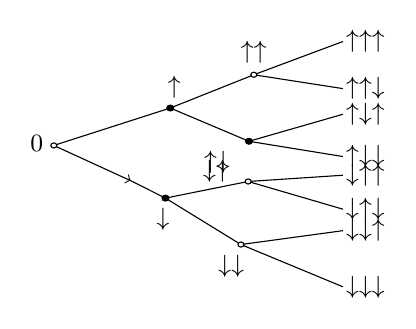
\begin{tikzpicture}[x=1.02cm,y=.88cm,every node/.style={font=\small,inner sep=1pt}]
\coordinate (O) at (0,0);
\coordinate (U) at (1.45,.54);
\coordinate (D) at (1.39,-.76);
\coordinate (UU) at (2.49,1.02);
\coordinate (UD) at (2.43,.06);
\coordinate (DU) at (2.42,-.52);
\coordinate (DD) at (2.33,-1.43);
\draw (O)--(U)--(UU)--(3.60,1.50) node[right] {\(\uparrow\uparrow\uparrow\)};
\draw (UU)--(3.60,.82) node[right] {\(\uparrow\uparrow\downarrow\)};
\draw (U)--(UD)--(3.60,.45) node[right] {\(\uparrow\downarrow\uparrow\)};
\draw (UD)--(3.60,-.16) node[right] {\(\uparrow\downarrow\downarrow\)};
\draw[->] (O)--(.96,-.51);
\draw (.96,-.51)--(D)--(DU)--(3.60,-.43) node[right] {\(\downarrow\uparrow\uparrow\)};
\draw (DU)--(3.60,-.92) node[right] {\(\downarrow\uparrow\downarrow\)};
\draw (D)--(DD)--(3.60,-1.23) node[right] {\(\downarrow\downarrow\uparrow\)};
\draw (DD)--(3.60,-2.04) node[right] {\(\downarrow\downarrow\downarrow\)};
\foreach \vertex in {O,UU,DU,DD}{\draw[fill=white] (\vertex) circle (.037);}
\foreach \vertex in {U,UD,D}{\fill (\vertex) circle (.051);}
\node[left] at (-.09,.03) {\(0\)};
\node[above] at (1.50,.63) {\(\uparrow\)};
\node[above] at (2.49,1.13) {\(\uparrow\uparrow\)};
\node[below] at (2.03,-.03) {\(\uparrow\downarrow\)};
\node[below] at (1.36,-.86) {\(\downarrow\)};
\node[above] at (2.02,-.58) {\(\downarrow\uparrow\)};
\node[below] at (2.21,-1.54) {\(\downarrow\downarrow\)};
\end{tikzpicture}}\endgroup}
\end{GelfandAdjacentEvidence}
\begin{GelfandAdjacentEvidence}{GELFAND-P000786}{6}


\(\ldots\}\,=\,\ldots\)
\Incomplete{GELFAND-P000786}{faint-formula-right}{Под числовой прямой видны правая фигурная скобка и знак равенства. Остальные слабые штрихи не дают прочитать выражение.}
\end{GelfandAdjacentEvidence}


\[
x\underset{\substack{\vert\\\text{earlier}\\\text{(раньше)}}}{\longleftarrow}y
\]
(т. е. \(x\) на пути от \(0\) к \(y\))

\(y]\) --- элемент мн-ва чисел, идущих раньше \(y\)

\uwave{Опер. усечения} --- \(x\) из меньшего числа стрелок

\(y\rceil\) число раньше \(y\), но больше его

\(y\rfloor\) ---\,\textquotedblleft\,--- и меньше его

\(x<y\) определено тоже
\begin{gather*}
\{y]\}=\{y\rfloor\}\cup\{y\rceil\},\\
\{y\rceil\}\cap\{y\rfloor\}=\Lambda
\end{gather*}

\underline{Пример:}

\uwave{Основное опр.:}


\Needspace{7\baselineskip}
\begin{GelfandAdjacentEvidence}{GELFAND-P000787}{1}
\SourcePage{GELFAND-P000787}{unlabelled}

\underline{Теор. 1}

(простая)

\(A,B\) --- \uwave{мн-ва чисел}

\(\forall a\in A,b\in B\); [зачёркнуто: \ldots{}] \(a<b\)
\Unclear{GELFAND-P000787}{theorem-one-cancellation}{Между точкой с запятой и неравенством густо перечёркнутый знак.}
\end{GelfandAdjacentEvidence}
\begin{GelfandAdjacentEvidence}{GELFAND-P000787}{2}


\uwave{Тогда} \(\exists x:\quad a<x<b.\)

\uwave{и сущ. единств. самое раннее} \(\underline{x}\).

\underline{Доказ-во:} трансфин. инд., смотрим \(x=0\) и если не смогли найти \(x\) до нек-рого места, то смотрим дальше.

\underline{Обозначение:}

\SourceFigure{GELFAND-P000787}{looped-braces}{%
\par\begingroup\color{black}\GelfandFitDiagram{\begin{tikzpicture}[every node/.style={inner sep=1pt}]
\node (notation) {\(\displaystyle \mathopen{{\scriptstyle\circ}\mkern-5mu\{} A:B \mathclose{\}\mkern-5mu{\scriptstyle\circ}}\quad\text{\sout{…}}\quad
  \text{или}\quad \mathopen{{\scriptstyle\circ}\mkern-5mu\{} a:b \mathclose{\}\mkern-5mu{\scriptstyle\circ}}\)};
\node[anchor=north west] at ([yshift=-2mm]notation.south west) {скобки с петлёй};
\end{tikzpicture}}\endgroup}
\end{GelfandAdjacentEvidence}
\begin{GelfandAdjacentEvidence}{GELFAND-P000787}{3}

\Unclear{GELFAND-P000787}{notation-cancellation}{Зачёркнутый знак перед «или» похож на «и».}
\end{GelfandAdjacentEvidence}
\begin{GelfandAdjacentEvidence}{GELFAND-P000787}{4}


\underline{Сложение.}

с пом. трансфин. индукции.

\underline{Теорема 2}
\[
x=\mathopen{{\scriptstyle\circ}\mkern-5mu\{} x\rfloor:x\rceil \mathclose{\}\mkern-5mu{\scriptstyle\circ}}
\]
(очевидно)

\underline{Опр. сложения.}
\[
x+y=\mathopen{{\scriptstyle\circ}\mkern-5mu\{} x\rfloor+y,\ x+y\rfloor:\ x\rceil+y,\ x+y\rceil \mathclose{\}\mkern-5mu{\scriptstyle\circ}}
\]

\underline{Теорема 3.}

а) \(0+0=\mathopen{{\scriptstyle\circ}\mkern-5mu\{} : \mathclose{\}\mkern-5mu{\scriptstyle\circ}}=0.\)

[Под формулой:] нет условий, значит вообще самое раннее

б) [зачёркнуто: \ldots{}] \(x+0=x\) по индукции
\Unclear{GELFAND-P000787}{zero-quantifier-cancellation}{Перечёркнутые штрихи напоминают \(\forall x\).}
\end{GelfandAdjacentEvidence}
\begin{GelfandAdjacentEvidence}{GELFAND-P000787}{5}


\underline{Д-во:}
\SourceFigure{GELFAND-P000787}{induction-pointer}{%
\par\begingroup\color{black}\GelfandFitDiagram{\begin{tikzpicture}[every node/.style={inner sep=1pt}]
\node {\(\displaystyle
\begin{aligned}
x+0&=\mathopen{{\scriptstyle\circ}\mkern-5mu\{} x\rfloor+0:x\rceil+0 \mathclose{\}\mkern-5mu{\scriptstyle\circ}}\\
&\underset{\text{инд.}}{=}\mathopen{{\scriptstyle\circ}\mkern-5mu\{} x\rfloor:x\rceil \mathclose{\}\mkern-5mu{\scriptstyle\circ}}
\underset{\substack{\nearrow\\\text{Теор. 2.}}}{=}x
\end{aligned}\)};
\end{tikzpicture}}\endgroup}
\end{GelfandAdjacentEvidence}
\begin{GelfandAdjacentEvidence}{GELFAND-P000787}{6}


В обычн. теории нет понятия раньше!

\(x+y\) --- простейшее число, монот. по каждому аргументу

а) монот. по \(x,y\)

б) среди всех таких самое раннее.

Вып. обычные св-ва
\begin{gather*}
x+y=y+x\\
(x+y)+z=x+(y\mathbin{\text{[?]}}z)
\end{gather*}
\Unclear{GELFAND-P000787}{associativity-sign}{Знак между \(y\) и \(z\) похож на \(\ge\). Чтение \(+\) также возможно.}
\end{GelfandAdjacentEvidence}


\uwave{Есть обр. операция.}

Противоп. к \(x\) --- обращ. стрелок\qquad
\(x+\operatorname{opp}.x=0\).


\Needspace{7\baselineskip}
\begin{GelfandAdjacentEvidence}{GELFAND-P000788}{1}
\SourcePage{GELFAND-P000788}{5}
\[
\uparrow+\uparrow=\mathopen{{\scriptstyle\circ}\mkern-5mu\{}1,1:\Lambda\}=\uparrow\uparrow
\]
\Unclear{GELFAND-P000788}{top-sum}{Начальные знаки перед и после плюса похожи на стрелки вверх; возможно чтение «1+1». Внутри скобок у единиц видны нижние засечки.}
\end{GelfandAdjacentEvidence}
\begin{GelfandAdjacentEvidence}{GELFAND-P000788}{2}


\underline{\underline{Упр.}}
\begin{gather*}
\uparrow\downarrow+\uparrow\downarrow=?\\
\widehat{\uparrow}+\downarrow\downarrow\downarrow=?
\end{gather*}

\underline{Умножение.}

\underline{Basic inequality} of \underline{mult'n.}

\[
r<s,\qquad u<v
\]
\Unclear{GELFAND-P000788}{basic-letter}{Знак перед \(<s\) условно передан буквой \(r\); по начертанию возможно \(\eta\).}
\end{GelfandAdjacentEvidence}
\begin{GelfandAdjacentEvidence}{GELFAND-P000788}{3}


Тогда
\[
ru+sv\mathrel{\text{[?]}}rv+su
\]
\Unclear{GELFAND-P000788}{basic-products}{Первые буквы в \(ru\) и \(rv\) обведены. Знак после \(sv\) переписан и похож на \(>\).}
\end{GelfandAdjacentEvidence}
\begin{GelfandAdjacentEvidence}{GELFAND-P000788}{4}


\(xy\) --- любое из 4-х \textup{[?]}\ \(\Rightarrow\) 4 нер-ва
\Unclear{GELFAND-P000788}{four-products-word}{После «4-х» возможно сокращение «слаг.» или «оп.».}
\end{GelfandAdjacentEvidence}
\begin{GelfandAdjacentEvidence}{GELFAND-P000788}{5}


\[
\begin{aligned}
x\cdot y={}&\mathopen{{\scriptstyle\circ}\mkern-5mu\{}x\rfloor\cdot y+x\cdot y\rfloor-x\rfloor\cdot y\rfloor,\\
&\phantom{\{}x\rceil\cdot y+x\cdot y\rceil-x\rceil\cdot y\rceil:\\
&\phantom{\{}x\rfloor\cdot y+x\cdot y\rceil-x\rfloor\cdot y\rceil,\\
&\phantom{\{}x\rceil\cdot y+x\cdot y\rfloor-x\rceil\cdot y\rfloor\}
\end{aligned}
\]
\Unclear{GELFAND-P000788}{recursion-mark}{Над запятой в конце третьей строки густая крестообразная помета. Её назначение неясно.}
\end{GelfandAdjacentEvidence}
\begin{GelfandAdjacentEvidence}{GELFAND-P000788}{6}


Вып. естеств. св-ва умножения.
\[
x\cdot0=\mathopen{{\scriptstyle\circ}\mkern-5mu\{}:\mathclose{\}\mkern-5mu{\scriptstyle\circ}}=0,\qquad x\cdot1=x
\]
\[
\begin{aligned}
x\cdot1&=\mathopen{{\scriptstyle\circ}\mkern-5mu\{}x\rfloor\cdot1+x\cdot0-x\rfloor\cdot0:\\
&\qquad x\rceil\cdot1+x\cdot0-x\rceil\cdot0\mathclose{\}\mkern-5mu{\scriptstyle\circ}}\\
&=\mathopen{{\scriptstyle\circ}\mkern-5mu\{}x\rfloor+0-0:x\rceil+0-0\mathclose{\}\mkern-5mu{\scriptstyle\circ}}=x
\end{aligned}
\]

Ассоциат., коммут., дистрибут. есть.

\uwave{Доказать дома.}

\underline{\underline{Совет.}} Технич. приём.

Док., что опред. [зачёркнуто: \sout{?}] [вписано над строкой со знаком вставки:] сложения „нечувствит. к скобкам“

\hfill\uwave{bracket indifferent}

\Unclear{GELFAND-P000788}{advice-cancellation}{Густо зачёркнутое сокращение допускает чтение «умн.».}
\end{GelfandAdjacentEvidence}


\begin{gather*}
x=\mathopen{{\scriptstyle\circ}\mkern-5mu\{}a:b\mathclose{\}\mkern-5mu{\scriptstyle\circ}}\\
y=\mathopen{{\scriptstyle\circ}\mkern-5mu\{}c:d\mathclose{\}\mkern-5mu{\scriptstyle\circ}}\\
x+y=\mathopen{{\scriptstyle\circ}\mkern-5mu\{}a+y,x+c:b+y,x+d\mathclose{\}\mkern-5mu{\scriptstyle\circ}}
\end{gather*}

Умножение тоже обл. этим св-вом.

\uwave{Ассоциат.}

Сущ. беск. большие и беск. малые числа.


\Needspace{7\baselineskip}
\begin{GelfandAdjacentEvidence}{GELFAND-P000789}{1}
\SourcePage{GELFAND-P000789}{unlabelled}
\[
\uparrow\uparrow\uparrow\ldots=\widehat{\uparrow}=\omega
\quad\text{--- простейшее беск. число.}
\]
\Unclear{GELFAND-P000789}{top-infinite-abbreviation}{Сокращение перед «число» читается предположительно как «беск.».}
\end{GelfandAdjacentEvidence}
\begin{GelfandAdjacentEvidence}{GELFAND-P000789}{2}


\[
\uparrow\downarrow\downarrow\ldots=\uparrow\widehat{\downarrow}=\varepsilon
\]

\SourceFigure{GELFAND-P000789}{nested-dyadic-brackets}{%
\par\begingroup\color{black}\GelfandFitDiagram{\begin{tikzpicture}[x=1cm,y=1cm,every node/.style={inner sep=1pt}]
\node at (.26,2.16) {\(1\)};
\draw (.06,1.87)--(.04,1.72)--(1.10,1.75) to[out=0,in=-75] (1.18,1.87);
\node at (.57,1.35) {\(\tfrac12\)};
\draw (0,1.18)--(-.02,.92)--(2.03,1.07) to[out=8,in=-77] (2.12,1.23);
\node at (1.20,.63) {\(1/4\)};
\end{tikzpicture}}\endgroup}
\end{GelfandAdjacentEvidence}
\begin{GelfandAdjacentEvidence}{GELFAND-P000789}{3}


\begin{gather*}
\omega\cdot\varepsilon=1\\
\omega+\varepsilon=\widehat{\uparrow}\uparrow\widehat{\downarrow}
\end{gather*}

Иногда можно сократить, но не всегда.

\uwave{Арифметика ординалов.}

[зачёркнуто: \sout{\ldots}] [вписано сверху:] ординалы: числа со стрелками \(\uparrow\) (без стрелок \(\downarrow\)).
\Incomplete{GELFAND-P000789}{ordinals-cancellation}{Слово под вставкой «ординалы» густо зачёркнуто и не читается.}
\end{GelfandAdjacentEvidence}
\begin{GelfandAdjacentEvidence}{GELFAND-P000789}{4}


Арифметика --- не обычная!

Обычная не коммутативна!

\SourceFigure{GELFAND-P000789}{ordinal-addition}{%
\par\begingroup\color{black}\GelfandFitDiagram{\begin{tikzpicture}[x=1cm,y=1cm,every node/.style={font=\small,inner sep=1pt}]
\node[anchor=east] at (.77,0) {\(\omega=1\)};
\node at (.99,0) {\(\oplus\)};
\node at (1.89,0) {\(\omega\ne\omega\)};
\node at (2.77,0) {\(\oplus\)};
\node[anchor=west] at (2.97,0) {\(1\)};
\node[anchor=west] at (3.74,0) {Это её дефект};
\draw (.99,-.25)--(1.27,-.67);
\draw (2.77,-.25)--(2.52,-.63);
\node[align=center] at (1.91,-.87) {обычная\\теория};
\end{tikzpicture}}\endgroup}
\end{GelfandAdjacentEvidence}
\begin{GelfandAdjacentEvidence}{GELFAND-P000789}{5}


Hessenburg прид. естеств. опр. слож. и умн. трансфин. чисел.
\Unclear{GELFAND-P000789}{hessenburg-spelling}{Последние буквы фамилии читаются предположительно как «burg».}
\end{GelfandAdjacentEvidence}
\begin{GelfandAdjacentEvidence}{GELFAND-P000789}{6}

\Unclear{GELFAND-P000789}{hessenburg-definition-abbreviation}{Сокращение после фамилии предположительно «прид.».}
\end{GelfandAdjacentEvidence}
\begin{GelfandAdjacentEvidence}{GELFAND-P000789}{7}


Оказалось, что оно совпад. с этим

\(\forall\) число, кроме \(0\), имеет обратное \(\frac1x\), \(x\ne0\).

\(\frac yx\) есть

\underline{\(\forall x>0\) есть \(\sqrt{x}\)} --- по инд. беск.
\Unclear{GELFAND-P000789}{sqrt-overwritten-variable}{Переменная после \(\forall\) переписана. Верхний знак читается как \(x\).}
\end{GelfandAdjacentEvidence}
\begin{GelfandAdjacentEvidence}{GELFAND-P000789}{8}

\Unclear{GELFAND-P000789}{sqrt-proof-abbreviation}{Сокращения после «по» предположительно «инд. беск.».}
\end{GelfandAdjacentEvidence}
\begin{GelfandAdjacentEvidence}{GELFAND-P000789}{9}


\(\forall\) многочлен, прин. в \(2^{\text{х}}\) точках знач. разных знаков, где-то между ними обр. в \(0\); но это беск. без непр. --- имеет щели, напр., между конеч. и беск. числами.
\Unclear{GELFAND-P000789}{polynomial-abbreviation}{Сокращение после «многочлен» читается предположительно как «прин.». После цифры 2 стоит надстрочное «х».}
\end{GelfandAdjacentEvidence}
\begin{GelfandAdjacentEvidence}{GELFAND-P000789}{10}


[слева зачёркнуто: \sout{\(?\)}] \(\overset{\ell}{\uparrow}\) --- „самое большое“
\(\longrightarrow\) [вписано сверху:] уже не сюрреал. число.
\Unclear{GELFAND-P000789}{lower-cancelled-symbol}{В зачёркнутом знаке видны верхняя петля и несколько пересекающихся штрихов.}
\end{GelfandAdjacentEvidence}
\begin{GelfandAdjacentEvidence}{GELFAND-P000789}{11}

\Unclear{GELFAND-P000789}{largest-number-superscript}{Петлеобразный знак над стрелкой предположительно \(\ell\).}
\end{GelfandAdjacentEvidence}
\begin{GelfandAdjacentEvidence}{GELFAND-P000789}{12}


\[
\widehat{\uparrow\downarrow}=\frac23\qquad\uparrow\downarrow\uparrow=\frac34
\]
\[
\widehat{\uparrow}\overset{\ell}{\downarrow}\quad\text{--- дыра}
\]
\Unclear{GELFAND-P000789}{gap-superscript}{Петлеобразный знак над стрелкой вниз предположительно \(\ell\).}
\end{GelfandAdjacentEvidence}


есть \(\exp x\); \(x^y\); \(\log\)


\Needspace{7\baselineskip}
\begin{GelfandAdjacentEvidence}{GELFAND-P000790}{1}
\SourcePage{GELFAND-P000790}{6}

Если \(x\) --- полож. беск., то
\[
2^x>x^n\qquad\text{для любого }n.
\]

\(x\) --- беск. малое \(\Rightarrow\)
\[
\exp x=\sum_{n\in\text{кон.}}\frac{x^n}{n!}
\]

\(x\) --- беск. малое, \(n\) --- вещ. \(\Rightarrow\) ряд
\(\sum x^n a_n\) сход. \(\forall a_n\)

Одно из возм. прил. теории:
\[
\int_x^{\overset{\ell}{\uparrow}}e^{-\xi^2}\,d\xi
=\sum\frac{n!}{x^n}
\]
\Unclear{GELFAND-P000790}{integral-upper-limit}{Над стрелкой в верхнем пределе интеграла виден петлеобразный знак, предположительно \(\ell\).}
\end{GelfandAdjacentEvidence}
\begin{GelfandAdjacentEvidence}{GELFAND-P000790}{2}


Всякое число \(=\) отнош. 2-х целых чисел \(\bigl(=\frac mn\bigr)\).

\[
\widehat{\uparrow}\downarrow=\omega-1
\]
\[
\lvert x]-x\rvert=1\qquad\text{--- опр. целого числа}
\]

\begin{gather*}
\exp x=\\
=\bigl\{0,\ \exp x]\cdot\sum_{m=1}^{n}\frac{(x-x]^{m}}{m!}
:\ \exp x]\bigg/\sum_{m=0}^{n}\frac{(x]-x)^m}{m!}
\end{gather*}
\Unclear{GELFAND-P000790}{exponential-delimiters}{После квадратной скобки в первой сумме закрывающая круглая скобка не видна. Заключительная фигурная скобка не написана.}
\end{GelfandAdjacentEvidence}



\Needspace{7\baselineskip}
\begin{GelfandAdjacentEvidence}{GELFAND-P000791}{1}
\SourcePage{GELFAND-P000791}{unlabelled}

\underline{13.11.78.}\qquad\underline{Сем. Гельфанда}

\uuline{А. Поляков}\qquad\uwave{2-мерная дискр. система.}

\[
(1)\qquad S=\operatorname{Tr}\sum_{\vec{x},\vec{\delta}}
g_{\vec{x}}^{-1}g_{\vec{x}+\vec{\delta}}
\]
\SourceFigure{GELFAND-P000791}{lattice-delta}{%
\par\begingroup\color{black}\GelfandFitDiagram{\begin{tikzpicture}[x=.83cm,y=.83cm]
\draw (-.79,2)--(3.23,2);
\draw (-.54,1)--(3.42,1);
\draw (-.44,0)--(3.46,0);
\draw (0,-.46)--(0,3.23);
\draw (1,-.55)--(1,3.06);
\draw (2,-.36)--(2,3.37);
\draw[->,very thick] (0,0)--(0,1);
\draw[->,very thick] (0,0)--(1,0);
\draw (-.11,-.11) circle (.063);
\node at (.48,-.93) {\(\vec{\delta}\)};
\end{tikzpicture}}\endgroup}
\end{GelfandAdjacentEvidence}
\begin{GelfandAdjacentEvidence}{GELFAND-P000791}{2}


\begin{align*}
(2)\qquad &g_{\vec{x}}\in GL(n,\mathbb R)\\
(3)\qquad &\partial_\mu F_{\mu\nu}(x)+[A_\mu,F_{\mu\nu}]=0\\
(4)\qquad &\sum_\delta\left\{\underbrace{g_{\vec{x}+\vec{\delta}}g_{\vec{x}}^{-1}}_{A_{\vec{x}\delta}}-
 g_{\vec{x}}g_{\vec{x}-\vec{\delta}}^{-1}\right\}=0
\end{align*}

\uwave{Сист. вполне интегр.} и есть беск. набор токов.
(есть \(L,A\)-пара и т. д.)
[под «есть» вписано: интегралы]
\Unclear{GELFAND-P000791}{integrability-note-end}{Последнее сокращение предположительно «т. д.».}
\end{GelfandAdjacentEvidence}
\begin{GelfandAdjacentEvidence}{GELFAND-P000791}{3}


\[
(5)\qquad\sum_\delta\left(J_{\vec{x}\delta}^{(k)}-J_{\vec{x}-\vec{\delta},\delta}^{(k)}\right)=0
\]

\uwave{Примеры токов:}
\begin{align*}
(6)_1\qquad &J_{\bar{x}\delta}^{(1)}=A_{x\delta}\\
(6)_2\qquad &J_{\bar{x}\delta}^{(2)}=\varepsilon_{\delta\gamma}A_{\bar{x}\gamma}+
\end{align*}
\Unclear{GELFAND-P000791}{current-indices}{Над \(x\) в индексах \((6)_1\) и \((6)_2\) видны короткие черты. У \(x\) в \(A_{x\delta}\) черты нет.}
\end{GelfandAdjacentEvidence}
\begin{GelfandAdjacentEvidence}{GELFAND-P000791}{4}

\Incomplete{GELFAND-P000791}{current-j2-ending}{Запись \((6)_2\) обрывается после плюса.}
\end{GelfandAdjacentEvidence}
\begin{GelfandAdjacentEvidence}{GELFAND-P000791}{5}


Для аб. группы и в пределе (непр.) по одной пер. --- цепочка Тода.

Здесь дискр. время. и неаб. случай

Цеп. Тода:
\[
(7)\qquad \mathcal{L}=\operatorname{Tr}\sum_s
\bigl(\dot{g}_s^{-1}\dot{g}_s+g_s^{-1}g_{s+1}\bigr)
\]
\Unclear{GELFAND-P000791}{kinetic-first-factor}{Над первым \(g_s\) в (7) видна точка слева от \(-1\). Порядок обращения и дифференцирования не указан скобками.}
\end{GelfandAdjacentEvidence}
\begin{GelfandAdjacentEvidence}{GELFAND-P000791}{6}


Положим
\[
(8)\qquad\left\{\begin{aligned}
A_s&=g_s^{-1}\dot{g}_s\\
B_s&=g_s^{-1}g_{s+1}
\end{aligned}\right.
\]

Условия нулевой кривизны:
\[
(9)\qquad\left\{\begin{aligned}
\dot{B}_s+A_sB_s-B_sA_{s+1}&=0\\
\dot{A}_s&=B_s-B_{s-1}
\end{aligned}\right.
\]
[справа от первой строки: (усл. \sout{связности?}); ниже вписано: 0-й кривизны]
\Unclear{GELFAND-P000791}{zero-curvature-cancellation}{Зачёркнутое слово предположительно «связности».}
\end{GelfandAdjacentEvidence}
\begin{GelfandAdjacentEvidence}{GELFAND-P000791}{7}


Найдём \(L_s\), \(M_s\), тоже уд. условию 0-й крив.
\[
(10)\qquad\dot{L}_s+M_sL_s-L_sM_{s+1}=0
\]
\Unclear{GELFAND-P000791}{lax-overwritten-sign}{Знак после \(\dot{L}_s\) переписан и предположительно читается как плюс.}
\end{GelfandAdjacentEvidence}
\begin{GelfandAdjacentEvidence}{GELFAND-P000791}{8}


Хотим:
\[
L_s(A,B,\lambda),\quad M_s(A,B,\lambda)
\]
\Unclear{GELFAND-P000791}{lax-parameters}{Знаки возле закрывающих скобок предположительно \(\lambda\); штрихи местами сливаются.}
\end{GelfandAdjacentEvidence}


так что \((10)\Rightarrow(9)\) и наоборот.

Тогда


\Needspace{7\baselineskip}
\begin{GelfandAdjacentEvidence}{GELFAND-P000792}{1}
\SourcePage{GELFAND-P000792}{17}

\[
(11)\qquad \frac{d}{dt}\left\{\prod_{s=-\infty}^{\infty}L_s\right\}=0
\]
\Unclear{GELFAND-P000792}{top-isolated-stroke}{Под произведением отдельный короткий штрих с точкой, похожий на \(i\).}
\end{GelfandAdjacentEvidence}
\begin{GelfandAdjacentEvidence}{GELFAND-P000792}{2}


произв. ф-я всех интегралов

\SourceFigure{GELFAND-P000792}{parallel-transport}{%
\par\begingroup\color{black}\GelfandFitDiagram{\begin{tikzpicture}[x=1cm,y=1cm]
\draw[->] (-1.3,0)--(2.3,0) node[below right] {\(s\)};
\draw[->] (0,-.59)--(0,1.33) node[right] {\(t\)};
\draw (1.47,.17)--(1.47,.74)--(-1.36,.74);
\draw[->] (-1.30,.68)--(-1.30,.02);
\end{tikzpicture}}\endgroup}
\end{GelfandAdjacentEvidence}
\begin{GelfandAdjacentEvidence}{GELFAND-P000792}{3}


\(L,M\) --- связности

\[
I(0)\underset{\mathrm{def}}{=}\prod L_s(0)
\]

Т. к.
\[
I(0)I^{-1}(\delta t)=1,
\]
то \(I(\delta t)=I(0)\) и \(I(t)\) --- интеграл дв-ния.

„Тупой способ“ поиска \(L,A\)-пары: итерации по \(\lambda\)

\underline{ответ}.

\[
(12)\qquad L_s=1+\lambda A_s-\lambda^2 B_sL_{s+1}^{-1}
\]

Итерир. по \(\lambda\)
\[
\prod_s(1+\lambda A_s)=1+\lambda\left(\sum A_s\right)
\]

\SourceFigure{GELFAND-P000792}{bracket-integral}{%
\par\begingroup\color{black}\GelfandFitDiagram{\begin{tikzpicture}[x=1cm,y=1cm,every node/.style={font=\small,inner sep=1pt}]
\node[anchor=base west] at (0,.79)
 {\((13)\quad\prod(1+\lambda A_s-\lambda^2B_s)\)};
\node[anchor=base west] (prefix) at (.43,.03)
 {\(=1+\lambda\sum A_s+\lambda^2\)};
\node[anchor=base west] (coef) at (prefix.base east)
 {\(\displaystyle\biggl(\sum_{s<s'} A_sA_{s'}-\sum B_s\biggr)\)};
\draw ([yshift=-1pt]coef.south west)--([yshift=-5pt]coef.south west)--
 ([yshift=-5pt]coef.south east)--([yshift=-1pt]coef.south east);
\node[below=6pt] at (coef.south) {\uwave{нетрив. интеграл}.};
\end{tikzpicture}}\endgroup}
\end{GelfandAdjacentEvidence}
\begin{GelfandAdjacentEvidence}{GELFAND-P000792}{4}

\Unclear{GELFAND-P000792}{product-expansions}{В обоих разложениях написаны знаки равенства. Продолжение по степеням не выписано.}
\end{GelfandAdjacentEvidence}
\begin{GelfandAdjacentEvidence}{GELFAND-P000792}{5}


\[
(14)\qquad \left\{\begin{aligned}
&L_s=e^{-\partial}+A_s+B_s e^\partial\\
&\text{\sout{\ldots}}\qquad M_s=B_s e^\partial
\end{aligned}\right.
\]
\Incomplete{GELFAND-P000792}{equation-14-cancellation}{В начале второй строки (14) густо зачёркнута запись. Её знаки не читаются.}
\end{GelfandAdjacentEvidence}
\begin{GelfandAdjacentEvidence}{GELFAND-P000792}{6}


Здесь \(e^\partial\) --- смещ. на 1 на решётке

\(L_s,M_s\) --- разностные операторы (Матр. Якоби)

\underline{Калибровочная теория.}

\SourceFigure{GELFAND-P000792}{gauge-lattice}{%
\par\begingroup\color{black}\GelfandFitDiagram{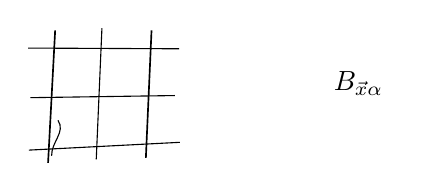
\begin{tikzpicture}[x=.9cm,y=.9cm]
\draw (-.30,0)--(1.83,.11);
\draw (-.28,.74)--(1.76,.77);
\draw (-.31,1.44)--(1.82,1.43);
\draw[semithick] (-.03,-.18)--(.07,1.69);
\draw (.65,-.13)--(.73,1.72);
\draw[semithick] (1.35,-.11)--(1.43,1.69);
\draw (.02,-.08) to[out=91,in=-56] (.11,.42);
\node at (4.35,.94) {\(B_{\vec{x}\alpha}\)};
\end{tikzpicture}}\endgroup}
\end{GelfandAdjacentEvidence}


\(\vec{x}\) --- точка, \(\alpha\) --- направление

(\(\alpha=1,\ldots,d\) ---\\
--- \(d\) --- размерность)

2-мерн. случай --- 2 напр.

(берутся только положительные)


\Needspace{7\baselineskip}
\begin{GelfandAdjacentEvidence}{GELFAND-P000793}{1}
\SourcePage{GELFAND-P000793}{unlabelled}

\[
(15)\qquad F_{\bar{x}\alpha\beta}=
B_{\bar{x},\alpha} B_{\bar{x}+\bar{\alpha},\beta}
B^{-1}_{\bar{x}+\bar{\beta},\alpha} B^{-1}_{\bar{x},\beta}
\]

Действие:
\[
(16)\qquad S=\sum_{\bar{x},\alpha,\beta}\operatorname{Tr} F_{\vec{x}\alpha\beta}
\]
[справа:] Классич. пред. \(\longrightarrow F^2\)
\Unclear{GELFAND-P000793}{action-classical-square}{Верхний знак слева от 2 предположительно прописное \(F\).}
\end{GelfandAdjacentEvidence}
\begin{GelfandAdjacentEvidence}{GELFAND-P000793}{2}


\SourceFigure{GELFAND-P000793}{action-margin}{%
\par\begingroup\color{black}\GelfandFitDiagram{\begin{tikzpicture}[every node/.style={inner sep=1pt,font=\small}]
\node[anchor=base west] (before) at (0,0) {\(\bigl(e^f=1+\)};
\node[anchor=base west] (linear) at (before.base east) {\(f\)};
\node[anchor=base west] at (linear.base east) {\({}+\tfrac{f^2}{2}\)};
\draw ([yshift=-2pt]linear.south)--([yshift=-9pt]linear.south);
\node[anchor=north west] at ([xshift=-7pt,yshift=-10pt]linear.south) {лин. член сокр. \(\bigr)\).};
\end{tikzpicture}}\endgroup}
\end{GelfandAdjacentEvidence}
\begin{GelfandAdjacentEvidence}{GELFAND-P000793}{3}

\Unclear{GELFAND-P000793}{action-exponential}{В скобках написан знак равенства. Ряд обрывается после \(f^2/2\).}
\end{GelfandAdjacentEvidence}
\begin{GelfandAdjacentEvidence}{GELFAND-P000793}{4}


\uwave{Ур-я движения:}

\SourceFigure{GELFAND-P000793}{motion-diagrams}{%
\par\begingroup\color{black}\GelfandFitDiagram{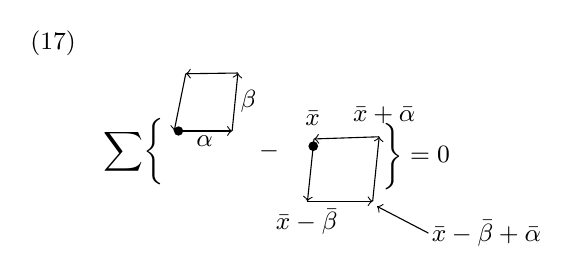
\begin{tikzpicture}[x=.92cm,y=.92cm,every node/.style={font=\small,inner sep=1pt}]
\node[anchor=base west] at (0,1.74) {\((17)\)};
\node at (1.48,.33) {\(\displaystyle\sum\biggl\{\)};
\draw[->] (2.03,.61)--(2.83,.61);
\draw[->] (2.83,.61)--(2.91,1.41);
\draw[->] (2.91,1.41)--(2.19,1.40);
\draw[->] (2.19,1.40)--(2.03,.61);
\fill (2.09,.61) circle (.064);
\node[below] at (2.45,.59) {\(\alpha\)};
\node[right] at (2.9,1.02) {\(\beta\)};
\node at (3.34,.33) {\(-\)};
\draw[->] (4.86,.53)--(3.96,.50);
\draw[->] (3.96,.50)--(3.87,-.36);
\draw[->] (3.87,-.36)--(4.77,-.36);
\draw[->] (4.77,-.36)--(4.86,.53);
\fill (3.95,.40) circle (.067);
\node[above] at (3.94,.64) {\(\bar{x}\)};
\node[above] at (4.93,.67) {\(\bar{x}+\bar{\alpha}\)};
\node[below] at (3.86,-.42) {\(\bar{x}-\bar{\beta}\)};
\node at (5.37,.26) {\(\displaystyle\biggr\}=0\)};
\node[anchor=west] (corner) at (5.54,-.80) {\(\bar{x}-\bar{\beta}+\bar{\alpha}\)};
\draw[->] (corner.west)--(4.83,-.43);
\end{tikzpicture}}\endgroup}
\end{GelfandAdjacentEvidence}
\begin{GelfandAdjacentEvidence}{GELFAND-P000793}{5}


Точкой выделено начало

\(\sum_\beta\), \(\alpha\) --- фиксир.\qquad
(\uwave{Ср.:} \(\nabla_\beta F_{\alpha\beta}=0\))
\Unclear{GELFAND-P000793}{motion-comparison-operator}{Переписанный знак предположительно \(\nabla\).}
\end{GelfandAdjacentEvidence}
\begin{GelfandAdjacentEvidence}{GELFAND-P000793}{6}


В 2-мерн. случае нет суммир.
\Unclear{GELFAND-P000793}{dimension-overwriting}{«мерн.» обведено. Более ранние штрихи неразличимы.}
\end{GelfandAdjacentEvidence}
\begin{GelfandAdjacentEvidence}{GELFAND-P000793}{7}


\((17)\) означает:
\[
\begin{aligned}
(17)_2\quad \sum\bigl\{&
B_{\bar{x},\alpha}
B_{\bar{x}+\alpha,\beta}
B^{-1}_{\bar{x}+\bar{\beta},\alpha}
B^{-1}_{\bar{x},\beta}\\
&-B^{-1}_{\bar{x}\beta}
B_{\bar{x}-\bar{\beta},\alpha}
B_{\bar{x}-\bar{\beta}+\bar{\alpha},\beta}
B^{-1}_{\bar{x}\alpha}
\bigr\}=0
\end{aligned}
\]
\Unclear{GELFAND-P000793}{expanded-fourth-factor}{В последнем множителе первого произведения \(\bar{x}\) обведено.}
\end{GelfandAdjacentEvidence}
\begin{GelfandAdjacentEvidence}{GELFAND-P000793}{8}

\Unclear{GELFAND-P000793}{motion-expanded-first-inverse}{В первом обратном множителе второго произведения индекс читается как \(\bar{x}\beta\).}
\end{GelfandAdjacentEvidence}
\begin{GelfandAdjacentEvidence}{GELFAND-P000793}{9}


\SourceFigure{GELFAND-P000793}{closed-contour-18}{%
\par\begingroup\color{black}\GelfandFitDiagram{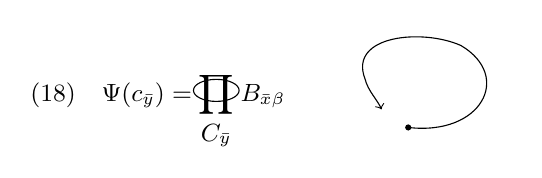
\begin{tikzpicture}[x=1cm,y=1cm,every node/.style={font=\small,inner sep=1pt}]
\node[anchor=base west] (lhs) at (0,0) {\((18)\quad\Psi(c_{\bar{y}})=\)};
\node[anchor=base west] (prod) at (lhs.base east) {\(\displaystyle\prod\)};
\draw ([yshift=4pt]prod.base) ellipse (.29 and .14);
\node[below=0pt] at (prod.south) {\(C_{\bar{y}}\)};
\node[anchor=base west] at (prod.base east) {\(B_{\bar{x}\beta}\)};
\begin{scope}[shift={(4.84,.06)}]
\draw[->] (0,-.39) .. controls (.93,-.50) and (1.33,.26) .. (.67,.65)
 .. controls (.18,.87) and (-.76,.78) .. (-.55,.23)
 .. controls (-.51,.07) and (-.39,-.04) .. (-.34,-.16);
\fill (0,-.39) circle (.039);
\end{scope}
\end{tikzpicture}}\endgroup}
\end{GelfandAdjacentEvidence}
\begin{GelfandAdjacentEvidence}{GELFAND-P000793}{10}

\Unclear{GELFAND-P000793}{contour-18-argument}{В аргументе буква предположительно строчная \(c\). Нижнее \(\bar{y}\) обведено.}
\end{GelfandAdjacentEvidence}
\begin{GelfandAdjacentEvidence}{GELFAND-P000793}{11}

\Unclear{GELFAND-P000793}{contour-18-product-subscript}{Под обведённым знаком произведения предположительно \(C_{\bar{y}}\).}
\end{GelfandAdjacentEvidence}
\begin{GelfandAdjacentEvidence}{GELFAND-P000793}{12}

\Unclear{GELFAND-P000793}{contour-18-b-subscript}{Переписанный знак в индексе \(B\) предположительно \(\bar{x}\).}
\end{GelfandAdjacentEvidence}
\begin{GelfandAdjacentEvidence}{GELFAND-P000793}{13}


Рассм.
\[
\Psi(c_y+\Pi_{\bar{x}\alpha\beta})
\]
\SourceFigure{GELFAND-P000793}{attached-square}{%
\par\begingroup\color{black}\GelfandFitDiagram{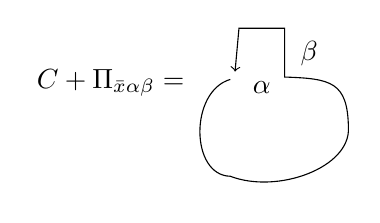
\begin{tikzpicture}[x=1cm,y=1cm]
\node[anchor=east] at (-.86,0) {\(C+\Pi_{\bar{x}\alpha\beta}=\)};
\draw[->] (-.40,.04)
 .. controls (-.92,-.11) and (-.91,-1.18) .. (-.40,-1.19)
 .. controls (.20,-1.42) and (1.13,-1.08) .. (1.10,-.57)
 .. controls (1.09,.01) and (.88,.05) .. (.29,.07)
 -- (.29,.69) -- (-.29,.69) -- (-.34,.14);
\node at (.00,-.06) {\(\alpha\)};
\node[right] at (.37,.37) {\(\beta\)};
\end{tikzpicture}}\endgroup}
\end{GelfandAdjacentEvidence}
\begin{GelfandAdjacentEvidence}{GELFAND-P000793}{14}

приклеили мал. квадратик

Теперь
\[
(19)\qquad\Psi(c+\Pi_{\bar{x}\alpha\beta})\Psi^{-1}(C)=
\]
\SourceFigure{GELFAND-P000793}{transport-19-diagram}{%
\par\begingroup\color{black}\GelfandFitDiagram{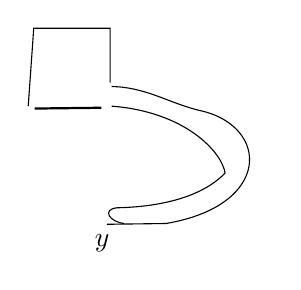
\begin{tikzpicture}[x=1cm,y=1cm]
\draw (-.70,.19)--(-.63,1.18)--(.34,1.18)--(.34,.49);
\draw[thick] (-.62,.16)--(.23,.17);
\draw (.36,.44)
 .. controls (.81,.43) and (1.10,.22) .. (1.50,.13)
 .. controls (2.36,-.07) and (2.40,-1.07) .. (1.05,-1.30)
 -- (.30,-1.31);
\draw (.36,.19)
 .. controls (1.29,.12) and (1.76,-.39) .. (1.80,-.66)
 .. controls (1.49,-.98) and (.94,-1.09) .. (.43,-1.10)
 .. controls (.23,-1.12) and (.33,-1.28) .. (.52,-1.30);
\node[below] at (.24,-1.32) {\(y\)};
\end{tikzpicture}}\endgroup
\par Разрывы возле квадрата и утолщённые концы штрихов сохранены. Направления в этих местах неясны.}
\end{GelfandAdjacentEvidence}
\begin{GelfandAdjacentEvidence}{GELFAND-P000793}{15}

\Unclear{GELFAND-P000793}{contour-19-case}{Первый знак похож на строчное \(c\) с петлёй. В аргументе обратной функции стоит \(C\).}
\end{GelfandAdjacentEvidence}
\begin{GelfandAdjacentEvidence}{GELFAND-P000793}{16}

\Unclear{GELFAND-P000793}{contour-19-alpha}{Обведённый индекс предположительно \(\alpha\).}
\end{GelfandAdjacentEvidence}
\begin{GelfandAdjacentEvidence}{GELFAND-P000793}{17}


напр. в т. \(\bar{x},\alpha\), перенес. в точку \(y\)

Ур-я запис. в виде:
\[
\begin{aligned}
(20)\qquad \sum_\beta\bigl\{&
\Psi(c+\Pi_{\bar{x}\alpha\beta})\Psi^{-1}(C)\\
&-\Psi(C)\Psi^{-1}(C-\Pi_{\bar{x}\alpha\beta})\bigr\}=0
\end{aligned}
\]
\Unclear{GELFAND-P000793}{contour-20-case}{Первый контур предположительно обозначен строчной \(c\).}
\end{GelfandAdjacentEvidence}
\begin{GelfandAdjacentEvidence}{GELFAND-P000793}{18}

\Unclear{GELFAND-P000793}{contour-20-overwritten-indices}{Обведённая пара индексов предположительно \(\alpha\beta\).}
\end{GelfandAdjacentEvidence}
\begin{GelfandAdjacentEvidence}{GELFAND-P000793}{19}


Получ. что-то вроде связности (тривиальной) в пр-ве контуров.
(т. е. [вписано над строкой:] матр. функция контура)

(ср. с (4))

\uwave{Непр. случай.}

\(\Psi[x_{\mu}(s)]\) --- функционал от кривой
(не зав. от параметризации)

[справа:] \(x(s)=(x_\mu(s));\quad \mu=1,2,3,4.\)
\Unclear{GELFAND-P000793}{continuous-overwritten-index}{Обведённый нижний индекс при \(x\) предположительно \(\mu\).}
\end{GelfandAdjacentEvidence}


Ток
\[
(21)\qquad \mathcal{F}_\mu(s,C)=\frac{\delta\Psi(x(s))}{\delta x_\mu(s)}\Psi^{-1}
\]


\Needspace{7\baselineskip}
\begin{GelfandAdjacentEvidence}{GELFAND-P000794}{1}
\SourcePage{GELFAND-P000794}{18}

\uuline{Ур-е:}
\[
(22)_1\qquad\frac{\delta\mathcal{F}_\mu(s,C)}{\delta x_\mu(s)}=0
\]

[справа]
\SourceFigure{GELFAND-P000794}{group-algebra-bracket}{%
\par\begingroup\color{black}\GelfandFitDiagram{\begin{tikzpicture}[x=1cm,y=1cm,every node/.style={font=\small,inner sep=1pt}]
\node[anchor=west] at (.59,.45) {\(\Psi\) прин. знач. в группе,};
\node[anchor=west] at (.59,-.16) {а \(\mathcal F\) --- в алгебре Ли};
\draw (.61,.71)--(.17,.71)--(0,-.45)--(.58,-.45);
\draw (.29,-.45)--(.38,.71);
\end{tikzpicture}}\endgroup}
\end{GelfandAdjacentEvidence}
\begin{GelfandAdjacentEvidence}{GELFAND-P000794}{2}


\(\Psi\) Инв. отн. параметризации: это запис. в виде
\[
(23)\qquad\frac{dx_\mu}{ds}\frac{\delta\Psi}{\delta x_\mu(s)}=0
\]

\begin{gather*}
\mathcal{F}_\beta=\Psi(c+\Pi_{\alpha\beta})\Psi^{-1}(c)\\
\sum_\beta\{\mathcal{F}_\beta(c)-\mathcal{F}_\beta(c-\Pi_{\alpha\beta})\}=0
\end{gather*}
\Unclear{GELFAND-P000794}{discrete-contour-case}{Буквы в аргументах предположительно строчные \(c\).}
\end{GelfandAdjacentEvidence}
\begin{GelfandAdjacentEvidence}{GELFAND-P000794}{3}


непр. предел даёт \((22)\).

\[
\Psi=p\,e^{\oint A_\mu\,dx_\mu}
\]
\[
(22)_2\qquad
\frac{\delta\mathcal{F}_\mu(s)}{\delta x_\nu(s')}
-\frac{\delta\mathcal{F}_\nu(s')}{\delta x_\mu(s)}
+[\mathcal{F}_\mu(s),\mathcal{F}_\nu(s')]=0
\]
\Unclear{GELFAND-P000794}{equation-22b-number}{Вторая цифра номера переписана. Верхняя запись предположительно \((22)_2\).}
\end{GelfandAdjacentEvidence}
\begin{GelfandAdjacentEvidence}{GELFAND-P000794}{4}


Действие
\[
(24)\qquad S'=\int\left(\frac{\delta\Psi^{-1}}{\delta x_\mu(s)}
\frac{\delta\Psi}{\delta x_\mu(s)}\right)(Dx_\mu(s))
\]
\Unclear{GELFAND-P000794}{action-number}{Вторая цифра совмещает штрихи, похожие на 4 и 1. Порядок переписи неясен.}
\end{GelfandAdjacentEvidence}
\begin{GelfandAdjacentEvidence}{GELFAND-P000794}{5}

\Unclear{GELFAND-P000794}{action-prime}{Косой штрих справа над \(S\) передан в обозначении \(S'\).}
\end{GelfandAdjacentEvidence}


Неясно, как определять

\uwave{Аккуратно:} 3 измерения.

(в \(4^{\underline{\text{х}}}\) ещё не до конца проверено).

Решаются ур-я \((22)_1\) --- \((22)_2\), где \(\mathcal{F}\) получ. по ф-ле (21), а \(\Psi\) удовл. усл. (23).

Поле Я.-М. --- киральное поле на пр-ве петель.

На петлях --- ф-я со знач. в конечномерной группе; для него ур-я главного кир. поля (\(\Psi\) --- такое поле) --- (22).

[вписано слева над строкой:] Если \(\Psi\) \uwave{из связности}
(\(\Leftrightarrow\) \(\Psi\) --- гомом. петель в группу) \(\Rightarrow\) получ. ур-я Я.-Миллса.

\uwave{Токи:} (\(\sim\) интегралы дв-ния):
\[
(25)\qquad
\frac{\delta\mathcal{J}^{(k)}_\mu(s,C)}{\delta x_\mu(s)}=0
\]


\Needspace{7\baselineskip}
\begin{GelfandAdjacentEvidence}{GELFAND-P000795}{1}
\SourcePage{GELFAND-P000795}{unlabelled}

\[
(26)\qquad\mathcal{J}^{(1)}_\mu=\mathcal{F}_\mu(s,C)
\]
\[
(27)\qquad\mathcal{J}^{(2)}_\mu=
\varepsilon_{\mu\nu\lambda}t_\nu(s)\mathcal{F}_\lambda(s,C)
+[\mathcal{F}_\mu(s),\chi]
\]

\(t\) --- касат. вектор к кривой

[\sout{\(\mathcal F\)}] \(\chi\) сейчас найдём
\Unclear{GELFAND-P000795}{cancel-before-chi}{Зачёркнутый знак похож на \(\mathcal F\).}
\end{GelfandAdjacentEvidence}
\begin{GelfandAdjacentEvidence}{GELFAND-P000795}{2}


Имеем:
\[
\begin{aligned}
(28)\qquad
\frac{\delta\mathcal{J}^{(2)}_\mu}{\delta x_\mu}
&=\underset{\substack{\Vert\\
\displaystyle\varepsilon_{\mu\nu\lambda}t_\nu[\mathcal{F}_\mu,\mathcal{F}_\lambda]}}
{\varepsilon_{\mu\nu\lambda}t_\nu(s)
\frac{\delta\mathcal{F}_\lambda(s,c)}{\delta x_\mu(s)}}\\[1ex]
&\quad+\left[\mathcal{F}_\mu(s,c),\frac{\delta\chi}{\delta x_\mu(s)}\right]
\end{aligned}
\]
\Unclear{GELFAND-P000795}{derivative-current-glyph}{Буква в числителе левой части переписана. Возможно \(\mathcal J\) или \(\mathcal F\).}
\end{GelfandAdjacentEvidence}
\begin{GelfandAdjacentEvidence}{GELFAND-P000795}{3}

\Unclear{GELFAND-P000795}{derivative-identity}{Две вертикальные черты связывают первое слагаемое с нижней записью. Перед \(\varepsilon\) в нижней строке отдельного коэффициента не видно.}
\end{GelfandAdjacentEvidence}
\begin{GelfandAdjacentEvidence}{GELFAND-P000795}{4}


Пусть
\[
(29)\qquad \frac{\delta\chi}{\delta x_\mu}=
-\varepsilon_{\mu\nu\lambda}t_\nu\mathcal{F}_\lambda
\]

Тогда
\[
(30)\qquad\mathcal{F}_\mu=\varepsilon_{\mu\nu\lambda}t_\nu
\frac{\delta\chi}{\delta x_\lambda}
\]

Это возможно при вып. \((22)_1\)

Получ. нелокальный закон сохранения. \quad Выраж-е. \(\chi\):
\Unclear{GELFAND-P000795}{figure-intro}{Сокращение перед \(\chi\) предположительно «Выраж-е.». Разделительный штрих неясен.}
\end{GelfandAdjacentEvidence}
\begin{GelfandAdjacentEvidence}{GELFAND-P000795}{5}


\SourceFigure{GELFAND-P000795}{loop-tail-expansion}{%
\par\begingroup\color{black}\GelfandFitDiagram{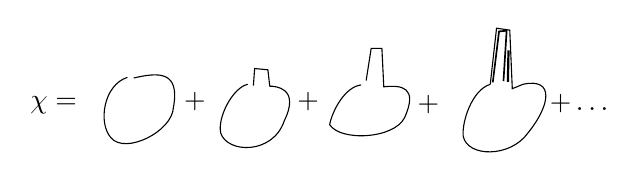
\begin{tikzpicture}[x=.8cm,y=.8cm,every node/.style={inner sep=1pt}]
\node at (0,.30) {\(\chi=\)};
\draw (1.17,.75)
 .. controls (.79,.63) and (.70,.02) .. (.91,-.21)
 .. controls (1.14,-.48) and (1.88,-.11) .. (1.90,.27)
 .. controls (2.01,.86) and (1.66,.83) .. (1.27,.74);
\node at (2.24,.37) {\(+\)};
\draw (3.08,.64)
 .. controls (2.85,.59) and (2.60,.13) .. (2.65,-.13)
 .. controls (2.75,-.46) and (3.48,-.48) .. (3.66,.06)
 .. controls (3.92,.59) and (3.51,.61) .. (3.43,.61)
 -- (3.40,.87)--(3.19,.89)--(3.17,.62);
\node at (4.04,.37) {\(+\)};
\draw (4.88,.63)
 .. controls (4.63,.60) and (4.43,.24) .. (4.38,.00)
 .. controls (4.55,-.27) and (5.40,-.23) .. (5.57,.11)
 .. controls (5.79,.60) and (5.52,.63) .. (5.24,.60)
 -- (5.21,1.21)--(5.04,1.21)--(4.96,.70);
\node at (5.95,.31) {\(+\)};
\draw (6.93,.64)
 .. controls (6.64,.55) and (6.48,.05) .. (6.50,-.18)
 .. controls (6.56,-.52) and (7.25,-.53) .. (7.53,-.13)
 .. controls (7.88,.30) and (7.96,.75) .. (7.45,.64)
 -- (7.28,.57)--(7.24,1.50)--(7.03,1.53)--(6.93,.64);
\draw[semithick] (6.97,.67)--(7.07,1.48)--(7.19,1.49)--(7.14,.69);
\draw[thick] (7.22,1.18)--(7.21,.68);
\node at (8.34,.34) {\(+\ldots\)};
\end{tikzpicture}}\endgroup
\par Короткие разрывы и утолщённые штрихи на последнем выступе переданы. Наконечники стрелок неразличимы.}
\end{GelfandAdjacentEvidence}
\begin{GelfandAdjacentEvidence}{GELFAND-P000795}{6}


(пристраивается квадр. по одному направлению)

Нелокальность 1-мерная.

\uwave{Контура}: 1. S. Mandelstam, Phys. Rev., 1968.

\hspace{1em}2. Минлос, Синай

[справа, на высоте пункта 1:] квант. Я.-М. в духе Фаддеева-Попова

\uwave{\(\gamma\)-пучок} (вместо \(L,A\)-пары)
\Unclear{GELFAND-P000795}{pencil-heading-sign}{Переписанный знак в заголовке предположительно \(\gamma\); возможно \(\lambda\).}
\end{GelfandAdjacentEvidence}
\begin{GelfandAdjacentEvidence}{GELFAND-P000795}{7}


\[
(31)\qquad
\frac{\delta\varphi}{\delta x_\mu(s)}
+Z\,\varepsilon_{\mu\nu\lambda}t_\nu\frac{\delta\varphi}{\delta x_\lambda}
=\mathcal{F}_\mu(s,C)\varphi(s,C)
\]
\Unclear{GELFAND-P000795}{equation-31-parameter}{Переписанный параметр похож на перечёркнутое \(Z\); регистр неясен.}
\end{GelfandAdjacentEvidence}
\begin{GelfandAdjacentEvidence}{GELFAND-P000795}{8}


\(Z\) --- произв. параметр
\Unclear{GELFAND-P000795}{parameter-note}{Буква в пояснении имеет похожую форму; регистр неясен.}
\end{GelfandAdjacentEvidence}
\begin{GelfandAdjacentEvidence}{GELFAND-P000795}{9}


Аналог. вид имеет:

\uwave{Станд. киральное поле}: (Pohlmayer, Захаров, Михайлов):
\[
\begin{aligned}
(32)\qquad A_\mu&=g^{-1}\partial_\mu g(x);\\
\left[\partial_\mu+Z\,\varepsilon_{\mu\nu}\partial_\nu\right]\varphi
&=A_\mu\varphi,\qquad\mu=1,2,\,..
\end{aligned}
\]
\Unclear{GELFAND-P000795}{equation-32-parameter}{Буква перед \(\varepsilon\) предположительно \(Z\); регистр неясен.}
\end{GelfandAdjacentEvidence}



\Needspace{7\baselineskip}
\begin{GelfandAdjacentEvidence}{GELFAND-P000796}{1}
\SourcePage{GELFAND-P000796}{19}

\((31)\) --- система ур-й, \(Z\) --- спектр. параметр.
\Unclear{GELFAND-P000796}{spectral-parameter-first}{Буква в пояснении обведена и похожа на перечёркнутое \(Z\). Регистр неясен.}
\end{GelfandAdjacentEvidence}
\begin{GelfandAdjacentEvidence}{GELFAND-P000796}{2}


Совместность \((31)\Rightarrow\) ур-я \((22)\).
\[
Z=0\quad\Rightarrow\quad\varphi=\Psi
\]
\Unclear{GELFAND-P000796}{spectral-parameter-zero}{Буква перед \(=0\) обведена и похожа на перечёркнутое \(Z\). В следующих формулах буква написана мельче.}
\end{GelfandAdjacentEvidence}
\begin{GelfandAdjacentEvidence}{GELFAND-P000796}{3}


\uwave{Интегралы} --- ?

На модели (32) посмотрим, как получ. интегралы.
\[
(32)\Leftrightarrow
\]
\[
(33)\qquad\partial_\mu\varphi
=\frac{A_\mu+z\varepsilon_{\mu\nu}A_\nu}{1-z^2}\,\varphi
\]
\[
(34)\qquad P\exp\oint_C\frac{A_\mu+z\varepsilon_{\mu\nu}A_\nu}{1-z^2}\,dx^\mu=1
\]
(упор. экспон)

Спец. выбор контура:
\SourceFigure{GELFAND-P000796}{contour-01}{%
\par\begingroup\color{black}\GelfandFitDiagram{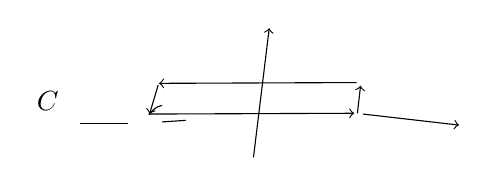
\begin{tikzpicture}[x=1cm,y=1cm]
\node[left] at (-2.54,.13) {\(C\)};
\draw (-2.39,-.15)--(-1.78,-.15);
\draw[->] (1.20,-.03)--(2.42,-.17);
\draw[->] (-.19,-.58)--(.01,1.06);
\draw[->] (1.12,.37)--(-1.39,.36);
\draw[->] (-1.40,.34)--(-1.51,-.03);
\draw[->] (-1.51,-.03)--(1.09,-.02);
\draw[->] (1.13,-.02)--(1.17,.33);
\draw (-1.35,-.13)--(-1.05,-.11);
\draw (-1.52,-.04) to[out=50,in=-170] (-1.35,.08);
\end{tikzpicture}}\endgroup
\par У левого нижнего угла видны дополнительные штрихи. Их назначение неясно.}
\end{GelfandAdjacentEvidence}
\begin{GelfandAdjacentEvidence}{GELFAND-P000796}{4}


\[
(35)\qquad\frac{d}{dt}\,P\exp\int_{-\infty}^{\infty}dx_1
\left\{\frac{A_1+zA_2}{1-z^2}\right\}=0
\]
Это производ. \underline{ф-я интегралов} дв-ния.

Обычные соотн. переносятся в „контурологию“.

Есть диагр. Фейнмана, где вместо линий --- поверхности.

Для своб. теории поля
\SourceFigure{GELFAND-P000796}{propagator-line}{%
\par\begingroup\color{black}\GelfandFitDiagram{\begin{tikzpicture}[x=1cm,y=1cm]
\fill (0,0) circle (.027);
\draw[->] (.12,0)--(2.35,0);
\node[below] at (.13,-.09) {\(x\)};
\node[below right] at (2.58,-.08) {\(x'\)};
\end{tikzpicture}}\endgroup}
\end{GelfandAdjacentEvidence}
\begin{GelfandAdjacentEvidence}{GELFAND-P000796}{5}

ф-я Грина \(G(x,x')\) удовл. ур-ю К.-Г..
\[
(36)\qquad (\partial_x^2-m^2)G(x,x')=\delta(x-x')
\]
\[
(37)\qquad G(x,x')\underset{|x-x'|\to\infty}{\sim}e^{-m|x-x'|}
\]

Здесь на контурах
\[
(38)\qquad \left\{\frac{\delta^2}{\delta x_\mu^2(s)}
-m^4\left(\frac{dx_\mu}{ds}\right)^2\right\}G(C)=0
\]
\Unclear{GELFAND-P000796}{string-denominator}{Переписанный знаменатель предположительно \(ds\).}
\end{GelfandAdjacentEvidence}

\[
(39)\qquad G(C)=\langle\Psi(C)\rangle
\]

Как найти конт. ф-ю Грина?

\uwave{Мат. задача:} \((38)\) --- „струнное“ ур-е К.-Г..

Гран. условие: убыв. при больших контурах:
\[
(40)\qquad G(C)\sim e^{-m^2 A(C)}
\]
(\(A(C)\) --- мин. площадь, натян. на контур \(C\))


\Needspace{7\baselineskip}
\begin{GelfandAdjacentEvidence}{GELFAND-P000797}{1}
\SourcePage{GELFAND-P000797}{unlabelled}

Пусть \(G\) зав. лишь от тензоров
\[
(41)\qquad \sigma_{\alpha\beta}=\oint_C x_\alpha\,dx_\beta
\]
\[
(42)\qquad \frac{\delta\sigma_{\alpha\beta}}{\delta x_\mu(s)}
=\delta_{\alpha\mu}\frac{dx_\beta}{ds}-\delta_{\beta\mu}\frac{dx_\alpha}{ds}
\]
\[
t_\mu(s)=\frac{dx_\mu}{ds}
\]
\[
(43)\qquad \text{\sout{\ldots}}\ t_\alpha t_\beta
\left[\frac{\partial^2}{\partial\sigma_{\alpha\gamma}\partial\sigma_{\beta\gamma}}
-m^4\delta_{\alpha\beta}\right]G=0
\]
\Unclear{GELFAND-P000797}{eq43-cancel}{Перед \(t_\alpha t_\beta\) зачёркнута запись, похожая на знак суммы с нижними индексами.}
\end{GelfandAdjacentEvidence}
\begin{GelfandAdjacentEvidence}{GELFAND-P000797}{2}


Пусть
\[
\pi_{\alpha\beta}=\frac{\partial}{\partial\sigma_{\alpha\beta}}
\]

Тогда получаем
\[
(44)\qquad \pi_{\alpha\beta}\pi_{\beta\gamma}
=\text{\sout{\(\tfrac14\pi^2_{\ldots}\delta_{\ldots}\)}}\quad C\delta_{\alpha\beta};
\]
\Unclear{GELFAND-P000797}{eq44-cancel}{После равенства зачёркнуты знаки, похожие на \(\frac14\), \(\pi^2\) и \(\delta\). Нижние индексы неясны.}
\end{GelfandAdjacentEvidence}
\begin{GelfandAdjacentEvidence}{GELFAND-P000797}{3}

\Unclear{GELFAND-P000797}{eq44-indices}{Индексы у незачёркнутого \(\delta\) справа читаются как \(\alpha\beta\).}
\end{GelfandAdjacentEvidence}
\begin{GelfandAdjacentEvidence}{GELFAND-P000797}{4}


Это возм. лишь при
\[
(45)\qquad \pi_{\alpha\beta}=\pm{}^*\pi_{\alpha\beta}
=\pm\varepsilon_{\alpha\beta\gamma\delta}\pi_{\gamma\delta}
\]

Отсюда ф-я лишь от
\[
(46)\qquad U_\pm=\sqrt{\sigma_{\alpha\beta}^2
\pm\sigma_{\alpha\beta}\,{}^*\sigma_{\alpha\beta}}
\]

Явное решение:
\[
G(U_+,U_-)
\]
выраж. через ф-и Бесселя.

[между строками:] Смотрим на бесконечности:

Мин. площадь
\[
(47)\qquad A_{\min}(C)=\sqrt{\sigma^2\pm\sigma\,{}^*\sigma}
\]
\(\sigma\) --- проекция на коорд. плоск.
\[
\sigma_{\alpha\beta}=\oint x_\alpha\,dx_\beta
\]
\[
A=\int\sqrt{\dot{x}^{\,2}x'^{\,2}-(\dot{x}x')^2}\,dt\,ds
\]

Ур-е Эйлера даёт
\[
A_{\min}(x(s))
\]
\Unclear{GELFAND-P000797}{final-argument}{В последней строке знаки аргумента обведены. Предположительно \(x(s)\).}
\end{GelfandAdjacentEvidence}



\Needspace{7\baselineskip}
\begin{GelfandAdjacentEvidence}{GELFAND-P000798}{1}
\SourcePage{GELFAND-P000798}{20}

Ур-е Гам.-Якоби
\[
\left(\frac{\delta A_{\min}}{\delta x_\mu(s)}\right)^2
=\left(\frac{dx_\mu}{ds}\right)^2
\]

Находим решение. (47) --- удовл. ур-ю Гам.-Якоби.

Для не слишком [\sout{\ldots}] перекруч. контуров \((47)\) --- решение.
\Incomplete{GELFAND-P000798}{text-cancel}{Между «слишком» и «перекруч.» зачёркнута короткая запись. Буквы не различаются.}
\end{GelfandAdjacentEvidence}


Синай утв., что у Куранта что-то есть.


\Needspace{7\baselineskip}
\begin{GelfandAdjacentEvidence}{GELFAND-P000799}{1}
\SourcePage{GELFAND-P000799}{unlabelled}

\underline{\underline{20.11.78.}}\qquad\underline{\underline{Сем. Гельфанда.}}

\SourceFigure{GELFAND-P000799}{palindrome-bracket}{%
\par\noindent
\(\left.\vcenter{\hbox{\scriptsize\shortstack[l]{%
«Торт с кофе не фокстрот»\\
«Сенсация: поп яйца снес»\\
«Я иду с мечем судия»}}}\right]\)
\enspace{\scriptsize\uwave{Палиндромы.}}
}
\end{GelfandAdjacentEvidence}
\begin{GelfandAdjacentEvidence}{GELFAND-P000799}{2}


\uwave{Кричевер:} инстантоны без расслоений.

\underline{\underline{А. С. Шварц.}}

1. \uwave{Квантовая} [вставлено над строкой: \uwave{теор. поля и}]
\uwave{статфиз.} --- наука о вычислении интеграла (стат. сумма)
\begin{equation*}
Z=\int e^{-S(A)}\,dA
\tag{1}
\end{equation*}
\(A\) пробегает пр-во траекторий или историй: \uwave{\(A=A(x,t)\)}.

\uwave{Смысл:} заменяем на конечномерный (сеточная аппрокс.) и переходим к пределу; \(a\) --- [\sout{\ldots}] шаг решётки.
\Unclear{GELFAND-P000799}{step-cancel}{Короткое слово перед «шаг решётки» зачёркнуто. Возможно, «шаг».}
\end{GelfandAdjacentEvidence}
\begin{GelfandAdjacentEvidence}{GELFAND-P000799}{3}


\uwave{КТП:} предел при \(a\to0\) не сущ.
\SourceFigure{GELFAND-P000799}{uv-arrow}{%
\par (ультрафиолетовые расход.)
\par\hspace{1em}\tikz[baseline=-.2ex]{\draw[<->] (0,0)--(.23,.31);}
\par решётка --- обрез. по импульсам.}
\end{GelfandAdjacentEvidence}
\begin{GelfandAdjacentEvidence}{GELFAND-P000799}{4}


Один из выходов: переходить к пределу для коррелляц. ф-й, т.е. вычислять
\begin{equation*}
\frac{\int\varphi(A)e^{-S(A)}\,dA}{\int e^{-S(A)}\,dA}
\tag{2}
\end{equation*}
(ф-и Грина или корреляц. ф-и).

\uwave{Важно:} предел отношения уже имеет смысл.

\underline{Ещё:} при снятии обрезания надо делать „перенормировку“, т.е. входящ. параметр \(\lambda_a\) менять в зав. от \(a\) при переходе к пределу.

\uwave{Сущ. 2 метода вычисления конт. инт.:}

\underline{теория возмущ.} и \underline{квазиклассика}

(на самом деле 1-е --- част. случай).

\uwave{Важный класс функционалов} \(S\), \uwave{к-рый оказ.}
\underline{\underline{вырожденным}},
т.е. допускающим. \(\infty\)-мерную группу симметрии:
\Unclear{GELFAND-P000799}{degeneracy-word}{Перед «вырожденным» читается сокращение «оказ.». После слова видна слабая точка перед запятой.}
\end{GelfandAdjacentEvidence}
\begin{GelfandAdjacentEvidence}{GELFAND-P000799}{5}

\[
g\in G\quad\leadsto\quad A\mapsto A^g
\]
\begin{equation*}
\underline{S(A^g)=S(A)}
\tag{3}
\end{equation*}

\uwave{Физические примеры:} калибровочные теории.

Чистая теория Я.-М.; \(A=(A_\mu(x))\), \(A_\mu\in\) алг. Ли конч. группы Ли.
\begin{equation*}
S(A)=\int\langle F_{\mu\nu},F^{\mu\nu}\rangle\,dV,
\tag{4}
\end{equation*}
где
\begin{equation*}
F_{\mu\nu}=\partial_\mu A_\nu-\partial_\nu A_\mu+[A_\mu,A_\nu]
\tag{5}
\end{equation*}
\Unclear{GELFAND-P000799}{curvature-index}{Индекс второго \(\partial\) густо обведён. Предварительное чтение --- \(\nu\).}
\end{GelfandAdjacentEvidence}



\Needspace{7\baselineskip}
\begin{GelfandAdjacentEvidence}{GELFAND-P000800}{1}
\SourcePage{GELFAND-P000800}{26}

\uwave{Группа симметрии:}

если \(g(x)\) --- ф-я со знач. в группе Ли,
то она порождает преобр. полей
\begin{equation*}
A_\mu\mapsto g A_\mu g^{-1}+g\,\partial_\mu(g^{-1})
\tag{6}
\end{equation*}
[над следующей строкой зачёркнуто: \sout{\ldots}]
\Incomplete{GELFAND-P000800}{upper-cancel}{Короткая запись над «Способ» закрыта густой штриховкой.}
\end{GelfandAdjacentEvidence}
\begin{GelfandAdjacentEvidence}{GELFAND-P000800}{2}


\uwave{Способ борьбы с вырожд. В случае эл.-магн. поля.}

«Потенциалы не им. смысла», наложим калибр. условие
\begin{equation*}
\partial_\mu A_\mu=0
\tag{7}
\end{equation*}
\uwave{Трудности:} трудно постр. теорию возмущений.

2. \uwave{Квазиклассика} \(\sim\) метод стац. фазы или Лапласа.

а) Давно реш. задача: как писать конт. интеграл (\uwave{Фаддеев и Попов})

[под строкой:] --- на физ. уровне строгости.

б) Мат. теория --- когда \(S\) квадратичен.

в) Применение к вычисл. инстантонного вклада.

г) Инварианты Рэя-Зингера.

а) \underline{Квантование выр. лагранжианов}.

\uline{Трудность:} интеграл расходится, т.к. объём орбит бесконечен.

\uwave{мораль:} выбрать калибр. условие --- трансверсаль к орбитам --- и инт. по ней.

\SourceFigure{GELFAND-P000800}{orbits-01}{%
\par\begingroup\color{black}\GelfandFitDiagram{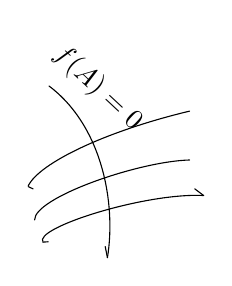
\begin{tikzpicture}[x=.94cm,y=.94cm,line cap=round,line join=round]
\draw (0,.61).. controls (.15,.92) and (1.05,1.35)..(2.18,1.62);
\draw (0,.60)--(.065,.57);
\draw (.086,.15).. controls (.08,.45) and (1.48,.94)..(2.18,.96);
\draw (.20,-.15).. controls (.06,.04) and (1.58,.52)..(2.37,.48);
\draw (.20,-.15)--(.27,-.145);
\draw (2.25,.57)--(2.37,.48);
\draw (.28,1.96).. controls (1.00,1.42) and (1.19,.37)..(1.07,-.36);
\draw (1.04,-.21)--(1.07,-.36);
\node[rotate=-43] at (.94,1.93) {\(f(A)=0\)};
\end{tikzpicture}}\endgroup
\par У правого конца нижней кривой и у нижнего конца поперечной кривой видны угловые штрихи. На схеме показаны их видимые стороны.}
\end{GelfandAdjacentEvidence}
\begin{GelfandAdjacentEvidence}{GELFAND-P000800}{3}


но: надо вставить множитель \(\underline{\underline{\delta(f(A))}}\).

Кроме того, надо вставить якобиан \(\Delta_f(A)\)
\begin{equation*}
\underline{\underline{\Delta_f(A)\delta(f(A))}}
\tag{8}
\end{equation*}
Приём Ф.-П. --- вычисление \(\Delta_f(A)\). (это не рассказывает)

\(\underline{\underline{f(A)=0}}\) --- ур-е трансверсали.

Для конечнократных инт. здесь --- \underline{\underline{теорема}}.

[слева приписано:] \underline{Другой приём.}

Рассмотрим снова интеграл (в конечнократном случае)
\begin{equation*}
\int_M e^{-S(A)}\,dA
=\int_{M/G}e^{-S(A)}\det(TT^*)^{1/2}\,dV,
\tag{9}
\end{equation*}
\Unclear{GELFAND-P000800}{eq9-determinant}{В (9) читается \(\det(TT^*)^{1/2}\). Штрих у \(\det\) не виден.}
\end{GelfandAdjacentEvidence}


где \(dV\) --- мера на мн-ии орбит, получ. из \uwave{станд. рим. метрики} на нём.

\(T\) --- оператор, получ. так: берём (считая действие свободным):
\[
T:\underset{\substack{\vert\\\text{алг. Ли}}}{\mathfrak g}
\xrightarrow{T_x}T_x(M)
\]
[справа:] отобр., получ. из действия группы.

Счит., что \(G\) действ. изометриями на \(M\).


\Needspace{7\baselineskip}
\begin{GelfandAdjacentEvidence}{GELFAND-P000801}{1}
\SourcePage{GELFAND-P000801}{unlabelled}

В физике возникает задача о вычислении методом Лапласа, т.е. об асимптотике
\begin{equation*}
\int e^{-\frac{1}{\alpha}S'(A)}\,dA\qquad
\text{при }\alpha\to0
\tag{10}
\end{equation*}
\Unclear{GELFAND-P000801}{exp-action}{После \(S\) в показателе (10) виден отдельный короткий штрих. Предварительное чтение --- \(S'\).}
\end{GelfandAdjacentEvidence}
\begin{GelfandAdjacentEvidence}{GELFAND-P000801}{2}


Надо знать стац. точки \(S'(A)\), называемые \uwave{инстантонами}.
\Unclear{GELFAND-P000801}{stationary-action}{Короткий штрих перед открывающей скобкой предварительно читается как штрих у \(S\).}
\end{GelfandAdjacentEvidence}
\begin{GelfandAdjacentEvidence}{GELFAND-P000801}{3}


Матем. задача такова: есть мн-ие стац. точек (и даже несколько многообразий) и даже \(\infty\)-мерные. Есть ещё сильное вырождение.

\underline{Примеры:}

1) Поле Я.-М.\qquad \(G=SU(2)\)

\(\forall q\) есть сем-во \(8q-3\) инстантонов помимо \(\infty\)-мерной симметрии.

\begin{equation*}
2)\qquad S(\vec n)=\frac{1}{f_0}\int(\partial_\mu\vec n)^2
\ \text{\sout{\ldots}}\ d^2x,
\quad \mu=0,1;\quad x=(x_0,x_1)
\tag{11}
\end{equation*}
\Incomplete{GELFAND-P000801}{eq11-cancel}{Между \((\partial_\mu\vec n)^2\) и \(d^2x\) густо зачёркнута запись. Видна петля слева. Саму запись прочитать не удаётся.}
\end{GelfandAdjacentEvidence}
\begin{GelfandAdjacentEvidence}{GELFAND-P000801}{4}


Надо вычислять гауссовы интегралы и возникает \(\underline{\underline{\det}}\).

Выр. лагранжиан даёт ещё один \(\det\) --- из Фаддеева-Попова --- это \(\underline{\det(TT^*)^{1/2}}\).

Детерминанты --- \(\infty\)-мерные; требуют аналит. прод. или перенормировки.

И они оказ. зависящими от выбора метрики.

Но: можно проследить за изменением \(\det\) при вариации метрики.

В \((11)\): \(\vec n=(n_1,n_2,n_3)\in S^2,\quad |\vec n|=1\).

Экстремали в \((11)\) найдены \uwave{Белавиным и Поляковым}.

Перейдём к стереогр. перем. на плоскости --- к сфере.

Получим \(\underline{\underline{w(z)}}\).

\underline{Ответ:} \uwave{экстремали}
\(\leftrightarrow\) \(w(z)\) --- \uwave{рациональные ф-и от} \(z\)!

\uwave{Объяснение:} есть топ. число \(N\) --- степень отображения

(\(\sim\) интеграл от якобиана).

Тогда простое вычисление показывает
\begin{equation*}
S'=c_1N+c_2\int\frac{1}{(1+|w|^2)^2}
\left|\frac{\partial w}{\partial\bar z}\right|^2,
\tag{12}
\end{equation*}
\Unclear{GELFAND-P000801}{eq12-measure}{Слева в (12) виден короткий штрих у \(S\). Предварительное чтение --- \(S'\). После квадрата модуля дифференциал не виден.}
\end{GelfandAdjacentEvidence}


отсюда всё следует.

Надо посчитать \(\det\).

Здесь нет калибровочной группы и есть один \(\det\). Асимпт. (10) даётся интегралом
\begin{equation*}
\int\det^{-1/2}(\ldots)\,d\mu_0,
\tag{13}
\end{equation*}
где \(\mu_0\) --- нек-рая мера на инстантонах.

\sout{Оказывается, что удобно}

Оператор строится по \(\forall\) рацион. ф-и как
[над строкой вставлено: опер. квадр. формы, соотв.] главной квадр. части ф-ла
\[
z=x_0+ix_1
\]
\begin{equation*}
z\xrightarrow{w}\mathrm{CP}(1)
\tag{14}
\end{equation*}


\Needspace{7\baselineskip}
\begin{GelfandAdjacentEvidence}{GELFAND-P000802}{1}
\SourcePage{GELFAND-P000802}{27}

\(T\mathrm{CP}(1)\) индуцирует расслоение на \(z\)-плоскости (по этому отобр.).

[под \(T\mathrm{CP}(1)\):] (голоморфное)

[справа:] \(w\) --- рац.
\begin{equation*}
\Delta=\bar\partial^{\,*}\bar\partial,\qquad
\bar\partial=\frac{\partial}{\partial\bar z}:\Lambda^{0,0}\to\Lambda^{0,1}
\tag{15}
\end{equation*}
[под правой частью:] \uwave{в формах со знач. в расслоении}.

Метрика тоже зависит от \(w\).

(индуцирована станд. метрикой \(\mathrm{CP}^{1}\))

\(w\) участвует реально только в \(*\).

\uwave{Надо сосчитать} \(\det\). Это дел. с пом. общей теории.

[зачёркнутый блок: \sout{\ldots}]
\Incomplete{GELFAND-P000802}{upper-cancel-block}{Внутри очерченного блока видны плотные горизонтальные и наклонные штрихи. Более ранняя запись не читается.}
\end{GelfandAdjacentEvidence}
\begin{GelfandAdjacentEvidence}{GELFAND-P000802}{2}


\(\det\) регуляризуем, одноврем. перенормировав \(f_0\) (пост. связи) в \((11)\).

Один из способов регуляризации: рассмотрим

[зачёркнуто: \sout{\(\zeta(A)=\)}]
\Unclear{GELFAND-P000802}{eq16-cancel}{Зачёркнутая запись предварительно читается как \(\zeta(A)=\). Штрихи конца пересекаются с зачёркиванием.}
\end{GelfandAdjacentEvidence}
\begin{GelfandAdjacentEvidence}{GELFAND-P000802}{3}

\begin{equation*}
\zeta(s)=\sum_{\lambda_i\ne0}\lambda_i^{-s}
\tag{16}
\end{equation*}
\(s=0\) --- точка аналит.
\begin{equation*}
\underline{\ln\det\underset{\mathrm{def}}{=}-\zeta'(0)}.
\tag{17}
\end{equation*}

Опер. \(\bar\partial\) „один и тот же“ для всех инстантонов с одинаковым топ. числом \(N\).

\uwave{Общее утверждение:} --- при изменении метрики можно проследить за изменением
\[
\det(A^*A)
\]
идея:

[\sout{\(\frac{d}{du}\operatorname{Sp}e^{-tA^*A}\)}]
\Unclear{GELFAND-P000802}{heat-variation-cancel}{В зачёркнутой записи предварительно читается \(\frac{d}{du}\operatorname{Sp}e^{-tA^*A}\). Показатель и знаменатель пересечены косыми штрихами.}
\end{GelfandAdjacentEvidence}
\begin{GelfandAdjacentEvidence}{GELFAND-P000802}{4}

\begin{equation*}
\frac{d}{du}A^*A=BA^*A+A^*CA
\tag{18}
\end{equation*}
Здесь \(B\) возникает из формулы, задающей вариацию скал. произведения:
\begin{equation*}
(u,v)=\langle u,v\rangle+\langle Bu,v\rangle.
\tag{19}
\end{equation*}

Вариацию \(\det A^*A\) выразим через
\(\underline{\operatorname{Sp}e^{-tA^*A}}\) с пом. интегр. Фруллани.

[над следующей формулой зачёркнуто: \sout{\(\ln\det A=\)}]
\Unclear{GELFAND-P000802}{eq20-cancel}{Зачёркнутая строка предварительно читается как \(\ln\det A=\). Последние штрихи перекрыты.}
\end{GelfandAdjacentEvidence}
\begin{GelfandAdjacentEvidence}{GELFAND-P000802}{5}

\begin{equation*}
\int_0^\infty\frac{e^{-ta}-e^{-tb}}{t}\,dt=\ln\frac ba
\tag{20}
\end{equation*}
(интеграл Фруллани).

или:
\begin{equation*}
\ln\det A=
\left(\int_\varepsilon^\infty\operatorname{Sp}e^{-tA^*A}\frac{dt}{t}\right)_{\text{рег. часть при }\varepsilon\to+0}
\tag{21}
\end{equation*}
\Unclear{GELFAND-P000802}{eq21-sign}{В (21) слева читается \(\ln\det A\). Перед интегралом не видно минуса или численного множителя.}
\end{GelfandAdjacentEvidence}



\Needspace{7\baselineskip}
\begin{GelfandAdjacentEvidence}{GELFAND-P000803}{1}
\SourcePage{GELFAND-P000803}{unlabelled}

\begin{equation*}
\begin{aligned}
\frac{d}{du}\operatorname{Sp}e^{-tA^*A}
&=-t\operatorname{Sp}\bigl[(BA^*A+A^*CA)e^{-tA^*A}\bigr]=\\
&=t\frac{d}{dt}\operatorname{Sp}\bigl[Be^{-tA^*A}\bigr]
 +\operatorname{Sp}\bigl[Ce^{-tAA^*}\bigr]
\end{aligned}
\tag{22}
\end{equation*}
\Unclear{GELFAND-P000803}{eq22-scope}{Во второй строке (22) скобка после следа с \(B\) закрывается перед плюсом. След с \(C\) записан отдельно, без видимого \(t\,d/dt\).}
\end{GelfandAdjacentEvidence}
\begin{GelfandAdjacentEvidence}{GELFAND-P000803}{2}


\(t\) --- сокр. с \(\frac{1}{t}\) в \((21)\)

и вылезают интегралы; соотв. коэфф. асимпт. Сили
\[
\ln\det A=\int_\varepsilon^\infty\operatorname{Sp}e^{-tA^*A}\frac{dt}{t}
 +\sum a_i\varepsilon^i+a_0\ln\varepsilon.
\]
\underline{\underline{Важен \(a_0\)}}.

\(t\to\infty\quad\Rightarrow\quad\) \uwave{нулевые моды}.

эта часть не считается.

Надо считать интеграл по \(d\mu_0\).

\(d\mu_0\) тоже надо считать! --- \uwave{это \(n\)-мерный \(\det\)}

Надо сосчитать \((4q+2)\)-мерный \(\det\) метрич. тензора.

Метрика в рац. ф-ях --- из метрики во всех ф-ях (в кас. пр-ве к ним) --- стандартной \(=\sum\) квадр. вариаций.

На самом деле \textbf{2} несосчит. части (из мод и из \(d\mu_0\)) сокращаются!!

Надо ещё сосчитать
\[
\int\Phi(\vec n)\det^{-1/2}(\ldots)\,d\mu_0.
\]
Зададим рац. ф-ю нулями и полюсами.
\[
\begin{array}{ll|l}
a_1\ldots a_n&\text{--- нули}&c\text{ --- асимпт. на }\infty.\\
b_1\ldots b_n&\text{--- полюса}&
\end{array}
\]
\[
\frac{
 \displaystyle\sum_q\int\varphi(\vec n)
 \frac{\prod |a_i-a_j|^2|b_i-b_j|^2}
 {\prod_{1\le i\le q}|a_i-b_j|^2}
 \frac{1}{(1+|c^2|)^2}\ldots
}{\displaystyle\sum_q\ldots}
\]
\Unclear{GELFAND-P000803}{ratio-indices}{Верхнее произведение записано без пределов. Под нижним стоит \(1\le i\le q\), а в множителе видны оба индекса \(i\) и \(j\). Степень в \(|c^2|\) находится внутри черт модуля.}
\end{GelfandAdjacentEvidence}
\begin{GelfandAdjacentEvidence}{GELFAND-P000803}{3}

\[
\varphi(\vec n)=n_\alpha(z')n_\beta(z'')
\]
Знаменатель --- стат. сумма кулоновского газа на плоскости.

В полюсах --- \(+\)-заряды

\hspace{1em}нулях --- \(-\)-заряды.

[справа:]
\[
\left(\prod_{\ldots}=\text{\sout{\ldots}}\ e^{\sum\ln\ldots}\right)
\]
\Incomplete{GELFAND-P000803}{lower-cancel}{Знак перед \(e\) густо зачёркнут. Видны угловые штрихи, но знак не устанавливается.}
\end{GelfandAdjacentEvidence}
\begin{GelfandAdjacentEvidence}{GELFAND-P000803}{4}


При одном знач. темп. (той самой!) это эквив. свободным \uwave{фермионам}.

[вставлено снизу: к-рое у нас]
\Unclear{GELFAND-P000803}{temperature-antecedent}{Сокращение в приписке под скобкой предварительно читается «к-рое».}
\end{GelfandAdjacentEvidence}



\Needspace{7\baselineskip}
\begin{GelfandAdjacentEvidence}{GELFAND-P000804}{1}
\SourcePage{GELFAND-P000804}{unlabelled}

\underline{\underline{27.11.78.}}\qquad\underline{Сем. Гельфанда.}

\uwave{Лев Николаевич Липатов}

об асимпт. диаграмм.

\underline{\underline{Захаров}}.

\uwave{Для интегрир. систем „общего полож.“ будет вып. вар. принцип}.

(все известные --- не общего положения)
\begin{equation*}
\begin{cases}
\Psi_\xi=U\Psi\\
\Psi_\eta=V\Psi
\end{cases}
\tag{1}
\end{equation*}
\[
\left.\begin{aligned}
U&=U(\xi,\eta,\lambda)\\
V&=V(\xi,\eta,\lambda)
\end{aligned}\right\}\quad\text{рац. ф-и по }\lambda
\]
\begin{equation*}
\begin{cases}
\displaystyle U=U_0+\sum_{n=1}^{N_1}\frac{U_n}{\lambda-\lambda_n},\\[1ex]
\displaystyle V=V_0+\sum_{n=1}^{N_2}\frac{V_n}{\lambda-\mu_n}
\end{cases}
\tag{2}
\end{equation*}
\[
\lambda_i\ne\lambda_j;\qquad\mu_i\ne\mu_j;\qquad\lambda_n\ne\mu_m
\]
\(\Psi,U,V\) --- матрицы

Инт. система:
\begin{equation*}
U_\xi-V_\eta+[U,V]=0
\tag{3}
\end{equation*}
\Unclear{GELFAND-P000804}{eq3-indices}{В (3) под \(U\) стоит \(\xi\), а под \(V\) --- \(\eta\).}
\end{GelfandAdjacentEvidence}


\uwave{Лакс. пары:} \(U\) имеет простой полюс в \(1^{\text{й}}\) точке,
\(V\) имеет полюс любого пор. в этой же точке


\Needspace{7\baselineskip}
\begin{GelfandAdjacentEvidence}{GELFAND-P000805}{1}
\SourcePage{GELFAND-P000805}{37}

[в начале строки зачёркнуто: \sout{\ldots}]
\Incomplete{GELFAND-P000805}{top-cancel}{Короткое слово закрыто несколькими горизонтальными чертами. Его буквы не различаются.}
\end{GelfandAdjacentEvidence}
\begin{GelfandAdjacentEvidence}{GELFAND-P000805}{2}


Тогда \(U,V\) можно сделать полиномами:
\[
U=U_0+U\lambda
\]
\[
V=P_n(\lambda)
\]
\Unclear{GELFAND-P000805}{top-u-coefficient}{У \(U\) перед \(\lambda\) не видно индекса.}
\end{GelfandAdjacentEvidence}
\begin{GelfandAdjacentEvidence}{GELFAND-P000805}{3}


Подробнее \((3)\) имеет вид:
\begin{equation*}
\begin{cases}
U_{0\eta}-V_{0\xi}+[U_0,V_0]=0\\
U_{n\eta}=[U_n,A_n]\\
V_{n\xi}=[V_n,B_n]
\end{cases}
\tag{4}
\end{equation*}
Здесь
\begin{equation*}
A_n=V\big|_{\lambda=\lambda_n},\qquad
B_n=U\big|_{\lambda=\mu_n}.
\tag{5}
\end{equation*}

Это сист. \(N_1+N_2+1\) ур-й относит. \(N_1+N_2+2\) величин.

Частично проинтегрируем: пусть \(U_n^{(0)}\) и \(V_n^{(0)}\) --- жорд. формы,
тогда
\begin{equation*}
U_n^{(0)}=U_n^{(0)}(\xi),\qquad
V_n^{(0)}=V_n^{(0)}(\eta)
\qquad\text{(в силу \((4)_{2,3}\))}
\tag{6}
\end{equation*}
\begin{equation*}
\begin{cases}
U_n=\varphi_n U_n^{(0)}\varphi_n^{-1},\\
V_n=\psi_n V_0^{(n)}\psi_n^{-1}
\end{cases}
\tag{7}
\end{equation*}
\Unclear{GELFAND-P000805}{tag7-overwriting}{Густо обведённый номер предварительно читается (7). Прежние штрихи внутри цифры не различаются.}
\end{GelfandAdjacentEvidence}
\begin{GelfandAdjacentEvidence}{GELFAND-P000805}{4}

\Unclear{GELFAND-P000805}{eq7-v-indices}{У среднего \(V\) во второй строке (7) нижний индекс \(0\), а верхний \((n)\).}
\end{GelfandAdjacentEvidence}
\begin{GelfandAdjacentEvidence}{GELFAND-P000805}{5}


Считаем матрицы \((6)\) \uwave{заданными}.

Сист. будет проинтегр., если будут найдены \(\varphi_n\) и \(\psi_n\) в \((7)\).

\(\varphi_n,\psi_n\) опред. неоднозначно: нужен один представитель.

Положим:
\begin{equation*}
\nabla_\eta=\frac{\partial}{\partial\eta}-V_0,\qquad
\nabla_\xi=\frac{\partial}{\partial\xi}-U_0.
\tag{8}
\end{equation*}
Тогда ур-я имеют вид
\begin{equation*}
\begin{cases}
\displaystyle\left(\nabla_\eta-\sum_{m=1}^{N_2}\frac{V_m}{\lambda_n-\mu_m}\right)\varphi_n=0\\[1.5ex]
\displaystyle\left(\nabla_\xi-\sum_{m=1}^{N_1}\frac{U_m}{\mu_n-\lambda_m}\right)\psi_n=0
\end{cases}
\tag{9}
\end{equation*}
[справа:] (подразум., что \(V_m,U_m\) выраж. через \((7)\))

Здесь классич. спинорные модели (для физиков). Действие:
\begin{equation*}
\begin{aligned}
S'=\int d\xi\,d\eta\,\operatorname{Sp}\Bigl[
 &\sum_{m=1}^{N_1}\varphi_n^{-1}\nabla_\eta\varphi_n U_n^{(0)}
 -\sum_{m=1}^{N_2}\psi_n^{-1}\nabla_\xi\psi_n V_n^{(0)}=\\
 &-\sum_{n=1}^{N_1}\sum_{m=1}^{N_2}\frac{U_m V_n}{\lambda_m-\mu_n}\Bigr]
\end{aligned}
\tag{10}
\end{equation*}
\Unclear{GELFAND-P000805}{action-prime}{У \(S\) в (10) виден приподнятый штрих, предварительно читаемый как \(S'\).}
\end{GelfandAdjacentEvidence}
\begin{GelfandAdjacentEvidence}{GELFAND-P000805}{6}

\Unclear{GELFAND-P000805}{eq10-indices}{В первых двух суммах предел \(m=1\), а в множителях индекс \(n\). В двойной сумме под \(N_1\) стоит \(n=1\), под \(N_2\) --- \(m=1\). Дробь читается как \(U_mV_n/(\lambda_m-\mu_n)\).}
\end{GelfandAdjacentEvidence}
\begin{GelfandAdjacentEvidence}{GELFAND-P000805}{7}

\Unclear{GELFAND-P000805}{eq10-end-sign}{Две черты в конце первой строки предварительно читаются как \(=\). Следующая строка начинается со знака минус.}
\end{GelfandAdjacentEvidence}



\Needspace{7\baselineskip}
\begin{GelfandAdjacentEvidence}{GELFAND-P000806}{1}
\SourcePage{GELFAND-P000806}{unlabelled}

Отсюда серии зак. сохранения (связ. с кол-вом полюсов)

\uwave{\(N_1+N_2\) серий.}

Простейш. сист. --- sin-Горд. --- полюса в \(0\) и \(\infty\).

\uwave{Гипотеза:} есть много гам. структур.

(как для КдФ --- беск. число гам. структур)

\underline{\underline{Липатов}}

\uwave{ЖЭТФ \underline{72}, 411, 1977.}

\begin{center}
\uwave{\(\displaystyle\alpha=\frac{e^2}{4\pi\hbar c}=\frac{1}{137}\)}
\end{center}
\begin{equation*}
\mathcal L=\int d^3x\,dt\left[
\frac{[\partial_\mu\varphi]^2}{2}
-\frac{m_0^2\varphi^2}{2}
-\lambda_0\frac{\varphi^4}{4!}\right]
\tag{1}
\end{equation*}

\uwave{Задача:} [\sout{\ldots}] вычисление ф-и Грина (в евклидовой области):
\Incomplete{GELFAND-P000806}{task-cancellation}{После «Задача» виден густо замазанный знак. Его начертание не устанавливается.}
\end{GelfandAdjacentEvidence}
\begin{GelfandAdjacentEvidence}{GELFAND-P000806}{2}

\begin{equation*}
G_{(c)}(x_1,\ldots,x_n)
=Z_0^{-1}\int\prod_x d\varphi(x)\,e^{-H(\varphi)}
\prod_{i=1}^{n}\varphi(x_i)
\tag{2}
\end{equation*}
\Unclear{GELFAND-P000806}{green-subscript}{Индекс в скобках предварительно читается как \((c)\). Видна угловатая черта с открытой правой стороной.}
\end{GelfandAdjacentEvidence}
\begin{GelfandAdjacentEvidence}{GELFAND-P000806}{3}

\[
H(\varphi)=\int d^4x\left[
\frac{(\partial_\sigma\varphi)^2}{2}
+\frac{\lambda_0\varphi^4}{4!}\,\text{\sout{]}}
+\frac{m_0^2\varphi^2}{2}\right]
\]
\Unclear{GELFAND-P000806}{hamiltonian-bracket}{После дроби с \(\lambda_0\) закрывающая квадратная скобка зачёркнута. Справа от последнего слагаемого стоит ещё одна скобка.}
\end{GelfandAdjacentEvidence}
\begin{GelfandAdjacentEvidence}{GELFAND-P000806}{4}


(\(=\mathcal L\) в евклидовой области)

Интеграл \((2)\) расходится. Но если сделать \(\lambda_0,m_0\)
зависим. от параметров обрезания, то ответ будет конечен (перенормировки!)

\(m_c^2\) --- полюс ф-и Грина (\(m_c\) --- [\sout{\ldots}] физ. масса).
\Incomplete{GELFAND-P000806}{mass-cancellation}{Перед «физ. масса» короткая запись пересечена несколькими чертами. Буквы не различаются.}
\end{GelfandAdjacentEvidence}
\begin{GelfandAdjacentEvidence}{GELFAND-P000806}{5}


\SourceFigure{GELFAND-P000806}{green-four-legs}{%
\par\begingroup\color{black}\GelfandFitDiagram{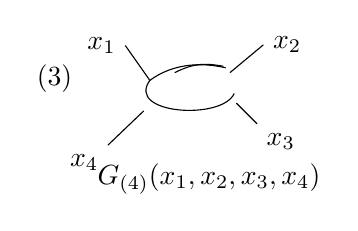
\begin{tikzpicture}[x=1cm,y=1cm,line cap=round]
\node at (-1.66,.17) {\((3)\)};
\draw (-.45,.15)..controls (-.76,-.28) and (.46,-.36)..(.62,-.02);
\draw (-.45,.15)..controls (-.15,.37) and (.21,.38)..(.51,.31);
\draw (-.13,.25)..controls (.11,.37) and (.25,.37)..(.48,.33);
\draw (-.45,.15)--(-.76,.59) node[left] {\(x_1\)};
\draw (.57,.25)--(.99,.60) node[right] {\(x_2\)};
\draw (.65,-.14)--(.91,-.40) node[below right] {\(x_3\)};
\draw (-.53,-.24)--(-.98,-.67) node[below left] {\(x_4\)};
\node at (.30,-1.10) {\(G_{(4)}(x_1,x_2,x_3,x_4)\)};
\end{tikzpicture}}\endgroup}
\end{GelfandAdjacentEvidence}
\begin{GelfandAdjacentEvidence}{GELFAND-P000806}{6}


\SourceFigure{GELFAND-P000806}{green-transform}{%
\par\begingroup\color{black}\GelfandFitDiagram{\begin{tikzpicture}[x=1cm,y=1cm]
\node[left] at (0,.12) {\(G_{(4)}\)};
\draw[->] (.08,.13)--(1.32,.13);
\node[align=center,font=\scriptsize] at (.69,-.34) {преобр.\\Фурье};
\node[right,align=left,font=\scriptsize] at (1.33,.11)
{\uwave{ф-я от \(p_1,p_2,p_3,p_4\)}};
\node[font=\scriptsize] at (.69,-.83) {в имп. прост.};
\end{tikzpicture}}\endgroup}
\end{GelfandAdjacentEvidence}
\begin{GelfandAdjacentEvidence}{GELFAND-P000806}{7}


(\(\sim\) рассеяние \(4^{\text{х}}\) частиц)

Полюс \(=\) [\sout{\ldots}] \(m_c^2\)
\Unclear{GELFAND-P000806}{pole-cancellation}{Зачёркнутое выражение перед \(m_c^2\) целиком не читается. Начальные штрихи могут относиться к \(m_0\).}
\end{GelfandAdjacentEvidence}


\uwave{ф-я \((3)\)} зависит лишь от \(p_j^2\) и \(p_i\cdot p_j\)
(из Лоренц.-инвар.)

и сод. \(\delta(p_1+p_2-p_3-p_4)\) (из сохр. импульса)

Вершинная ф-я Грина:
\begin{equation*}
\Gamma=\frac{G(p_1,p_2,p_3,p_4)}{G(p_1)G(p_2)\ldots G(p_4)}
\tag{4}
\end{equation*}
(после вын. \(\delta\)-ф-и)

По теории возмущений (при \(\lambda_0=0\)) получим
\begin{equation*}
G^0(p)=\frac{1}{p^2+m^2}.
\tag{5}
\end{equation*}


\Needspace{7\baselineskip}
\begin{GelfandAdjacentEvidence}{GELFAND-P000807}{1}
\SourcePage{GELFAND-P000807}{38}

[зачёркнуто: \sout{\ldots}]
\[
\frac{[G(p_1)\ldots G(p_4)]^{1/2}}{[G^0(p_1)\quad G^0(p_4)]^{1/2}}
\]
\Incomplete{GELFAND-P000807}{top-cancellation}{Перед верхней дробью густо зачёркнута запись, возможно \(\Gamma(p)\). Штрихи между скобками не различаются.}
\end{GelfandAdjacentEvidence}
\begin{GelfandAdjacentEvidence}{GELFAND-P000807}{2}


\[
\lambda(p_i))=\lambda_0\Gamma(p_i))
\frac{[\prod_1^4G(p_i]^{1/2}}{[\prod_1^4G_0(p_i)]^{1/2}}
\quad\text{--- \underline{заряд} (инвариантный)}
\]
\Unclear{GELFAND-P000807}{lambda-arguments}{Аргументы \(\lambda\) и \(\Gamma\) предварительно читаются как \(p_i\) с двумя следами закрывающих скобок. В числителе после \(p_i\) видна квадратная скобка без отдельной круглой.}
\end{GelfandAdjacentEvidence}
\begin{GelfandAdjacentEvidence}{GELFAND-P000807}{3}

\[
p=(p_1,p_2,p_3,p_4)
\]
\(\lambda_0\) подб. так, чтобы физ. заряд был конечен (и все ф-и Грина тоже)

Парадокс \uwave{Ландау и Померанчука}:
если не по теории возм., а оставить главный \(\ln\), то получ.
\[
\lambda_\mu=\frac{\lambda_0}{1+\frac{3}{2}\frac{\lambda_0}{16\pi^2}
\ \text{\sout{\ldots}}\ \ln\frac{\Lambda}{\mu^2}}.
\]
\Incomplete{GELFAND-P000807}{denominator-cancellation}{Запись перед \(\ln\) густо зачёркнута. Её знаки не различаются.}
\end{GelfandAdjacentEvidence}
\begin{GelfandAdjacentEvidence}{GELFAND-P000807}{4}


[справа от формулы:] \(\mu\) --- опр. точка: \(p_ip_j=\mu^2\), \(p_i^2=(\ldots)\mu^2\).

\((\cdot)\) из \((\sum p_i)^2=0\).

\[
\lambda_0>0\quad\Rightarrow\quad\lambda_\mu\longrightarrow\infty
\quad\text{при }\Lambda\longrightarrow\infty
\quad\text{(т.е. снятии обрезания).}
\]
\Unclear{GELFAND-P000807}{landau-limit}{В дроби после \(1\) стоит плюс, а ниже при \(\Lambda\to\infty\) написано \(\lambda_\mu\to\infty\).}
\end{GelfandAdjacentEvidence}
\begin{GelfandAdjacentEvidence}{GELFAND-P000807}{5}


То же в кв. электродин. [\sout{\ldots}]
(ни при какой затрав. \(\lambda_0\) не получ. \(\frac{1}{137}\))
\Incomplete{GELFAND-P000807}{electrodynamics-cancellation}{Между «электродин.» и открывающей скобкой запись пересечена косыми штрихами. Она не читается.}
\end{GelfandAdjacentEvidence}


Необходима асимптотика коэфф. в ряде теории возмущений, возник. для
\[
\psi=\frac{d\lambda_\mu}{d\ln\frac{\Lambda}{\mu^2}}
=a_2\lambda_\mu^2+a_3\lambda_\mu^3+\ldots
\]
асимпт. по \(k\) при \(k\to+\infty\) есть

Первые 4 явно найдены.

\uwave{Идея:} метод Лапласа для континуального интеграла

\uline{Нер-во Соболева:}
\[
\left[\int(\partial_\sigma\varphi)^2\,d^4x\right]^2
\geq\frac{32\pi^2}{3}\int\varphi^4(x)\,d^4x
\]
рав-во достигается при
\[
\varphi=\frac{c_1}{(x-x_0)^2+\lambda^2}
\]

[\underline{\underline{Вставка Захарова}}\quad
\uwave{\(\Delta\varphi+\varphi^3=0\)}
--- из ур-й Я.-М. получается]


\Needspace{7\baselineskip}
\begin{GelfandAdjacentEvidence}{GELFAND-P000808}{1}
\SourcePage{GELFAND-P000808}{unlabelled}

\underline{4.12.78г.}\qquad \uwave{Сем. Гельфанда.}

\underline{\underline{A. Guichardet}}

\underline{\underline{Расширения предст. топ. групп.}}

1. \uwave{Расш. модулей над дискр. группами}.

\(E,F\) --- 2 \(G\) модуля.
\Unclear{GELFAND-P000808}{module-count}{Густо обведённая цифра между «—» и \(G\) предварительно читается как 2.}
\end{GelfandAdjacentEvidence}
\begin{GelfandAdjacentEvidence}{GELFAND-P000808}{2}


Расш. \(E\) с помощью \(F\) --- это 3-й \(G\)-модуль \(H\), такой что
\(H\supset F\) и \(H/F\cong E\) или точная послед.
\begin{equation*}
0\longrightarrow F\longrightarrow H\longrightarrow E\longrightarrow0
\tag{1}
\end{equation*}
2 расш. эквив., если \(\exists\) изом., такой, что диагр. коммут.

\SourceFigure{GELFAND-P000808}{equivalence-diagram}{%
\par\begingroup\color{black}\GelfandFitDiagram{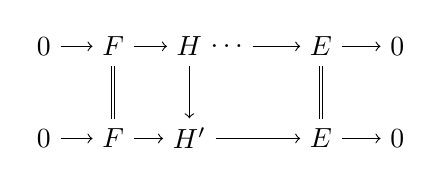
\begin{tikzpicture}[x=.88cm,y=.78cm]
\node (z) at (0,1) {\(0\)};
\node (f) at (1,1) {\(F\)};
\node (h) at (2.1,1) {\(H\)};
\node (cancel) at (2.64,1) {\sout{\(\ldots\)}};
\node (e) at (4,1) {\(E\)};
\node (end) at (5.1,1) {\(0\)};
\node (zb) at (0,-.5) {\(0\)};
\node (fb) at (1,-.5) {\(F\)};
\node (hb) at (2.1,-.5) {\(H'\)};
\node (eb) at (4,-.5) {\(E\)};
\node (endb) at (5.1,-.5) {\(0\)};
\draw[->] (z)--(f);
\draw[->] (f)--(h);
\draw[->] (cancel.east)--(e);
\draw[->] (e)--(end);
\draw[->] (zb)--(fb);
\draw[->] (fb)--(hb);
\draw[->] (hb)--(eb);
\draw[->] (eb)--(endb);
\draw[double] (f.south)--(fb.north);
\draw[->] (h.south)--(hb.north);
\draw[double] (e.south)--(eb.north);
\end{tikzpicture}}\endgroup
\par Справа от верхнего \(H\) зачёркнута запись. Возможно, ещё одна буква \(H\).}
\end{GelfandAdjacentEvidence}
\begin{GelfandAdjacentEvidence}{GELFAND-P000808}{3}


Тривиальное расширение:
\begin{center}
\uwave{\(H=F\oplus E\)}
\end{center}

\uwave{Сильное расширение:} \((1)\) --- сильное, если \(\exists\) сечение
[\sout{\(E\xrightarrow{s}H\)}]
\Unclear{GELFAND-P000808}{section-cancel}{Зачёркнутая стрелка предварительно читается \(E\xrightarrow{s}H\). Правая буква пересечена косыми штрихами.}
\end{GelfandAdjacentEvidence}
\begin{GelfandAdjacentEvidence}{GELFAND-P000808}{4}


\SourceFigure{GELFAND-P000808}{section-diagram}{%
\par\begingroup\color{black}\GelfandFitDiagram{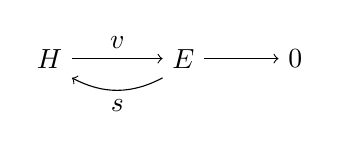
\begin{tikzpicture}[x=1cm,y=1cm]
\node (h) at (0,0) {\(H\)};
\node (e) at (1.7,0) {\(E\)};
\node (z) at (3.12,0) {\(0\)};
\draw[->] (h)--node[above] {\(v\)}(e);
\draw[->] (e)--(z);
\draw[->] (e.south west) to[bend left=28] node[below] {\(s\)} (h.south east);
\end{tikzpicture}}\endgroup}
\end{GelfandAdjacentEvidence}
\begin{GelfandAdjacentEvidence}{GELFAND-P000808}{5}


\uwave{\(v\cdot s=\mathrm{id}\)};
\uwave{\(s\) --- морфизм групп} (а не \uwave{\(G\)-модулей})
\Unclear{GELFAND-P000808}{projection-symbol}{Знак в \(v\cdot s=\mathrm{id}\) и над стрелкой предварительно читается как \(v\).}
\end{GelfandAdjacentEvidence}


[под словом «групп» вставлено: (абелевых).]

(если \(s\) --- морф. \(G\)-мод., то расширение тривиально)

Мн-во классов эквив. [вставлено над строкой: сильных] расширений:
\uwave{\(\operatorname{Ext}^1(E,F)\)}

Метод: когомологии

\(\operatorname{Hom}(E,F)\) --- морф. групп

это \(G\)-модуль: действие задаётся так
\[
gu=g\cdot u\cdot g^{-1}
\]


\Needspace{7\baselineskip}
\begin{GelfandAdjacentEvidence}{GELFAND-P000809}{1}
\SourcePage{GELFAND-P000809}{43}

\underline{\underline{Опр.}}
\[
H^1(G,\operatorname{Hom}(E,F))
\]
\uwave{1-коциклы}
\[
f:G\longrightarrow\operatorname{Hom}(E,F)
\]
\begin{equation*}
f(gg')=f(g)+g\circ f(g')\circ g^{-1}.
\tag{2}
\end{equation*}
\Unclear{GELFAND-P000809}{cocycle-g-strokes}{Первое \(g\) после плюса в (2) обведено у нижней петли. Читается \(g\), соседний штрих не различается отдельно.}
\end{GelfandAdjacentEvidence}
\begin{GelfandAdjacentEvidence}{GELFAND-P000809}{2}


\(Z^1\) --- все коциклы.

1-кограницы (\(B^1\)).
\[
\exists\,u\in\operatorname{Hom}(E,F):\quad
f(g)=g\circ u\circ g^{-1}-u
\]
\[
H^1\underset{\mathrm{def}}{=}Z^1/B^1.
\]
Сущ. соответствие (вз. однозн.)
\[
H^1\cong\operatorname{Ext}^1(E,F)
\]
По коциклу \(\varphi\) постр. расширение:
\[
H=F\oplus E
\]
\begin{equation*}
g(f,e)=(gf+\varphi(g)g\cdot e,\quad g\cdot e).
\tag{3}
\end{equation*}
или в матрицах:
\[
\begin{pmatrix}
V_g&\varphi(g)U_g\\
0&U_g
\end{pmatrix}
\quad\text{--- \uwave{так строится действие}.}
\]
\Unclear{GELFAND-P000809}{group-block-glyphs}{В правом верхнем углу последняя буква предварительно читается как \(U_g\), как и на диагонали. Нижний левый знак открыт справа и предварительно читается как \(0\).}
\end{GelfandAdjacentEvidence}
\begin{GelfandAdjacentEvidence}{GELFAND-P000809}{3}


\(V_g,U_g\) --- [\sout{\ldots}] предст. \(G\) в соотв. пр-вах.
\Unclear{GELFAND-P000809}{representation-count}{Перед «предст.» видна зачёркнутая или обведённая запись, возможно цифра 2.}
\end{GelfandAdjacentEvidence}
\begin{GelfandAdjacentEvidence}{GELFAND-P000809}{4}


Отсюда можно получить опр. коцикла.

2 предст. эквив. \(\Longleftrightarrow\) коциклы гомологичны

2. \uwave{Расширения модулей над алгебрами Ли}.

[справа:]
\[
X\longrightarrow\begin{pmatrix}A(X)&f(X)\\0&B(X)\end{pmatrix}
\]
\Unclear{GELFAND-P000809}{lie-block-glyphs}{В правом верхнем углу буква обведена и предварительно читается как \(f\). Нижний левый знак открыт справа и передан как \(0\).}
\end{GelfandAdjacentEvidence}


коцикл --- линейное отображение \(f:\mathfrak g\longrightarrow\operatorname{Hom}(E,F)\)

\uwave{опр. коцикла} имеет вид:
\begin{equation*}
f([X,Y])=X\circ f(Y)-f(Y)\circ X-Y\circ f(X)+f(X)\circ Y.
\tag{4}
\end{equation*}
\(f\) --- кограница, если \(\exists\,u\)
\begin{equation*}
f(X)=X\circ u-u\circ X.
\tag{5}
\end{equation*}

\underline{Лемма} 1. \(E,F\) имеют [вставлено над строкой: различные]
инфинитезим. характеры \(\Rightarrow\)
\[
\Rightarrow\quad\operatorname{Ext}^1(E,F)=0
\]
\(\mathfrak g\longmapsto U(\mathfrak g)\)\qquad
универс. обёрт. алгебра, \(Z(\mathfrak g)\) --- её центр


\Needspace{7\baselineskip}
\begin{GelfandAdjacentEvidence}{GELFAND-P000810}{1}
\SourcePage{GELFAND-P000810}{unlabelled}
Пусть \(\underline{\underline{u\in Z(\mathfrak g)}}\) действует в \(E\) как умн. на скаляр
\[
\text{\uwave{\(\displaystyle u\cdot e=\chi(u)e\)}}
\]
Тогда \(\chi\in\operatorname{Hom}(Z(\mathfrak g),\mathbb C)\)

\uwave{это инфинит. характер.}

\(H^1(\mathfrak g,\operatorname{Hom}(E,F))\) — \uwave{есть}

\(H^1(\mathfrak g,\mathfrak h,\operatorname{Hom}(E,F))\),\qquad
\(\mathfrak h\subset\mathfrak g\)

[Справа на поле: \(\ldots\).]
\Unclear{GELFAND-P000810}{right-margin-mark}{Изолированный неразборчивый знак}
\end{GelfandAdjacentEvidence}
\begin{GelfandAdjacentEvidence}{GELFAND-P000810}{2}


(описывает расширения, тривиальные с точки зрения \(\mathfrak h\)).
\[
Z^1(\mathfrak g,\mathfrak h,\operatorname{Hom}(E,F))
=\{f\in Z^1(\mathfrak g,\ldots),\quad f|_{\mathfrak h}=0\}
\]
\[
H^1(\mathfrak g,\mathfrak h,\ldots)\in H^1(\mathfrak g,\ldots)
\]
\Unclear{GELFAND-P000810}{relative-relation}{Между группами в рукописи стоит знак \(\in\).}
\end{GelfandAdjacentEvidence}
\begin{GelfandAdjacentEvidence}{GELFAND-P000810}{3}


\uline{Комментарии}:

\uwave{Можно с пом. дифференциала}:
\[
(df)(x,y)=f([x,y])-xf(y)+yf(x)
\]
\(xf(y)\) — \uuline{действие} алг. Ли

(выше запис. с пом. \uwave{коммутатора})

3. \uwave{Расширения модулей над группами Ли}.

\(G\)-модуль — топ. вект. пр-во, \(G\) действ. непрерывно.

\(\mathfrak g\) — алг. Ли

\(\begin{array}{@{}l@{}} K\subset G\\[-3pt] \vert\\[-3pt]\text{макс. комп. подгр.},\end{array}\)

\(\mathfrak k\) — соотв. алг.,

\(E,F\) — т.в.п.

\uwave{1-я идея.}\quad \uwave{коциклы}
\[
f:G\longrightarrow\operatorname{Hom}(E,F)
\]
\((e,g)\longmapsto f(g)e\)\qquad непр. по \(g\) и \(e\).

\uwave{2-я идея}: вместо \(E,F\) — пр-во дифф. векторов \(E_\infty,F_\infty\)

хороши, но не совершенны при \(\underline{\underline{E=\mathbb C}}\). Пусть так.
\Unclear{GELFAND-P000810}{differentiable-vectors-phrase}{Рукопись не уточняет смысл слов «не совершенны».}
\end{GelfandAdjacentEvidence}
\begin{GelfandAdjacentEvidence}{GELFAND-P000810}{4}


\uline{Теорема}:
\SourceFigure{GELFAND-P000810}{theorem-attributions}{%
\par\begingroup\color{black}\GelfandFitDiagram{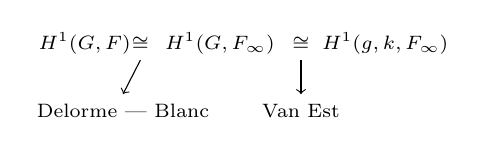
\begin{tikzpicture}[x=1cm,y=.85cm, every node/.style={font=\scriptsize}]
\node[anchor=west,inner sep=0] at (0,0) {\(H^1(G,F)\)};
\node (a) at (1.30,0) {\(\cong\)};
\node[inner sep=0] at (2.31,0) {\(H^1(G,F_\infty)\)};
\node (b) at (3.34,0) {\(\cong\)};
\node[anchor=west,inner sep=0] at (3.60,0) {\(H^1(\mathfrak g,\mathfrak k,F_\infty)\)};
\node (db) at (1.08,-1) {Delorme — Blanc};
\node (ve) at (3.34,-1) {Van Est};
\draw[->] (a.south) -- (db.north);
\draw[->] (b.south) -- (ve.north);
\end{tikzpicture}}\endgroup\par}
\end{GelfandAdjacentEvidence}
\begin{GelfandAdjacentEvidence}{GELFAND-P000810}{5}

\Unclear{GELFAND-P000810}{theorem-arrows}{Первая буква алгебры в правой группе обведена и читается предположительно как \(\mathfrak g\).}
\end{GelfandAdjacentEvidence}
\begin{GelfandAdjacentEvidence}{GELFAND-P000810}{6}


\uwave{Для \(\mathbb R\) нетрив.}
\[
\begin{pmatrix}1&at\\0&1\end{pmatrix}
\]
— \uwave{расширение} трив. \(\mathbb R\)-модуля тривиальным

нет соотв. предст. групп и алгебр

(\uwave{в когом.}: надо брать когом., трив.
[зачёркнуто: \(\ldots\)] на компактной подгруппе).
\Incomplete{GELFAND-P000810}{bottom-cancellation}{слово закрыто штрихами}
\end{GelfandAdjacentEvidence}



\Needspace{7\baselineskip}
\begin{GelfandAdjacentEvidence}{GELFAND-P000811}{1}
\SourcePage{GELFAND-P000811}{44}
\uwave{Несовершенство}:

даже если \(F\) — неприв. унит. предст., то может быть
\[
\underline{\dim H^1(G,F)\mathrel{\overset{?}{=}}+\infty}
\]
\Unclear{GELFAND-P000811}{dimension-sign}{Знак имеет две почти горизонтальные черты и наложенный угловой штрих. По начертанию возможно \(\geq\); равенство согласуется со следующим примером.}
\end{GelfandAdjacentEvidence}
\begin{GelfandAdjacentEvidence}{GELFAND-P000811}{2}


\uline{Пример}\qquad \(G\) — афф. гр. прямой\quad
\quad \(ax+b\)
\Unclear{GELFAND-P000811}{affine-mark}{Знак похож на \(R\), но отдельные штрихи могут быть зачёркиванием.}
\end{GelfandAdjacentEvidence}
\begin{GelfandAdjacentEvidence}{GELFAND-P000811}{3}


\(B^1\) всюду плотно в \(Z^1\), но \(\underline{\underline{\dim Z^1/B^1=+\infty}}\)

Причина: \(F\) слабо содержит тривиальное предст.

Для полупростых групп всё хорошо,
[зачёркнуто: \(\ldots\)]
\Incomplete{GELFAND-P000811}{semisimple-cancellation}{исходные знаки не читаются}
\end{GelfandAdjacentEvidence}
\begin{GelfandAdjacentEvidence}{GELFAND-P000811}{4}


Пусть \(G\) — полупростая;

\uwave{унит. неприв. предст}.

Известно, когда \(H^1=0\).

Для неполупростых:
\[
\text{\uwave{\(\displaystyle SO_0(m,n)\)}}
\]
не сущ. неунит. предст. с ненулевыми когом.

\Unclear{GELFAND-P000811}{nonsemisimple-context}{В рукописи при \(SO_0(m,n)\) стоят рубрика «Для неполупростых» и сокращение «неунит.»}
\end{GelfandAdjacentEvidence}
\begin{GelfandAdjacentEvidence}{GELFAND-P000811}{5}


\uwave{Доб. недостаток \(1^{\text{й}}\) идеи}.

Лемма об инфинит. хар. неверна!

Контрпример есть [зачёркнуто: \(\ldots\)] для \(SL(2,\mathbb R)\)
\Unclear{GELFAND-P000811}{counterexample-cancellation}{Возможно «все», но поперечные штрихи закрывают часть букв.}
\end{GelfandAdjacentEvidence}
\begin{GelfandAdjacentEvidence}{GELFAND-P000811}{6}


\uwave{2-я идея}: верна лемма об инфин. хар-рах, но

[На левом поле, зачёркнуто: \(\ldots\)]
\Unclear{GELFAND-P000811}{second-margin-cancellation}{Возможно, повторено «но».}
\end{GelfandAdjacentEvidence}
\begin{GelfandAdjacentEvidence}{GELFAND-P000811}{7}

\[
H^1(G,\operatorname{Hom}(E_\infty,F_\infty))
\]
трудно вычислить.

\[
L_\infty^2\longrightarrow L_\infty^2
\]
[Слева и строкой ниже, зачёркнуто: \sout{\(L_\infty^2\longrightarrow\ldots\)};\quad
\sout{Задача \(\ldots\)}]
\Incomplete{GELFAND-P000811}{long-cancellations}{Начало верхней записи предположительно \(L_\infty^2\), дальше видна стрелка. В нижней строке после «Задача» слова и знаки закрыты штрихами.}
\end{GelfandAdjacentEvidence}
\begin{GelfandAdjacentEvidence}{GELFAND-P000811}{8}


\uline{3-я идея}.
\[
E,F\rightsquigarrow E_K,F_K
\]
(векторы, включ. в конечномерные предст. \(K\)).

\Incomplete{GELFAND-P000811}{k-cancellations}{Два текстовых фрагмента зачёркнуты. Отдельные петли видны, но слова не читаются.}
\end{GelfandAdjacentEvidence}
\begin{GelfandAdjacentEvidence}{GELFAND-P000811}{9}


\(K\)-конечные;\qquad \uwave{\(K\) — макс. комп. подгруппа}

\(SL(2,\mathbb R)\) — для всех непр. модулей Хариш-Чандры можно выч.
\Unclear{GELFAND-P000811}{hc-abbreviation}{Сокращение «непр.» предположительно означает «неприводимых».}
\end{GelfandAdjacentEvidence}
\begin{GelfandAdjacentEvidence}{GELFAND-P000811}{10}

\[
H^1(\mathfrak g,\mathfrak k,\operatorname{Hom}(E_K,F_K))
\]
алгебра без топологии.

4. \uwave{Случай полупрямого произведения}.
\[
G=B\underset{\text{полупр.}}{\times}A\underset{\sigma}{=}B\wedge A,
\qquad B=\mathbb R^n,\quad A\text{ — гр. Ли}
\]
\Unclear{GELFAND-P000811}{product-equality-mark}{Знак под равенством предположительно читается как \(\sigma\), возможно \(g\). Между \(B\) и \(A\) стоит \(\wedge\).}
\end{GelfandAdjacentEvidence}


(напр., афф. гр. прямой).

\(B^*\) — сопр. пр-во,\qquad \(\langle b,x\rangle\) — двойств.

\(X=A\)-орбита в \(B^*\)

(действие \(A\) в \(B\) есть и опр. полупрямого произвед.)


\Needspace{7\baselineskip}
\begin{GelfandAdjacentEvidence}{GELFAND-P000812}{1}
\SourcePage{GELFAND-P000812}{unlabelled}
[Слева от даты зачёркнуто: \(\ldots\).]
\Incomplete{GELFAND-P000812}{date-cancellation}{слово или цифры не читаются}
\end{GelfandAdjacentEvidence}
\begin{GelfandAdjacentEvidence}{GELFAND-P000812}{2}


\uuline{12/II-79 г.}\qquad \uline{Сем. Гельфанда.}

\uwave{Что нужно знать?} (по \uline{А. А. Белавину}):

I.\quad \uline{Фейнман}.

\hspace{1em}1.\quad Курс для домохозяек, гг. 8, 9.

\hspace{1em}2.\quad Статистическая физика

\hspace{1em}3.\quad Интегралы по путям (с Гиббсом)
\Unclear{GELFAND-P000812}{feynman-coauthor}{В рукописи «Гиббсом». Вероятно, имеется в виду А. Р. Хиббс, соавтор книги Фейнмана об интегралах по путям.}
\end{GelfandAdjacentEvidence}
\begin{GelfandAdjacentEvidence}{GELFAND-P000812}{3}


\(\overline{\underline{\mathrm{II}}}\).\quad \uline{Хуанг} «Статист. механика» Глава: Решение Онзагера.

\(\overline{\underline{\mathrm{III}}}\).\quad \uline{Ф. Клейн} «Лекции по истории математики в \uuline{XIX} столетии»

[Зачёркнут номер: \(\ldots\)]
\Unclear{GELFAND-P000812}{list-cancellation}{возможно IV}
\end{GelfandAdjacentEvidence}
\begin{GelfandAdjacentEvidence}{GELFAND-P000812}{4}

[4. Книжки с синими кубиками на обложке (на белом фоне)

\hspace{1em}(Фейнман: «Фунд. зак. физики»).]

\SourceFigure{GELFAND-P000812}{list-placement-arrow}{%
\par\begingroup\color{black}\GelfandFitDiagram{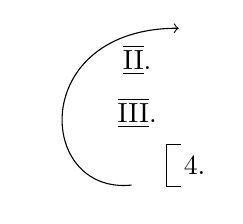
\begin{tikzpicture}[x=.8cm,y=.83cm]
\draw[->] (1.12,0) .. controls (-.4,-.15) and (-.52,2.4) .. (1.87,2.4);
\node at (1.21,1.91) {\(\overline{\underline{\mathrm{II}}}\).};
\node at (1.21,1.10) {\(\overline{\underline{\mathrm{III}}}\).};
\draw (1.9,.62) -- (1.67,.62) -- (1.67,-.02) -- (1.9,-.02);
\node at (2.12,.3) {4.};
\end{tikzpicture}}\endgroup\par
Стрелка по левому полю ведёт от зачёркнутого номера к промежутку перед II.}
\end{GelfandAdjacentEvidence}
\begin{GelfandAdjacentEvidence}{GELFAND-P000812}{5}


\(\overline{\underline{\mathrm{IV}}}\).\quad \uline{Дирак} Статья в книге «Монополь Дирака»

\hspace{1em}книги. «Лекции по квантовой механике»

\hspace{1em}«[знаки повтора слов «Лекции по»] теории поля»

\hspace{1em}«Общая теория относительности»

\(\overline{\underline{\mathrm{V}}}\).\quad \uline{Ахиезер}, \uline{Берестецкий} «Квантовая электродинамика»

\hspace{1em}(надо знать содержание, но не читать)

\(\overline{\underline{\mathrm{VI}}}\).\quad Сборник «Частицы и компенсирующие поля», Статья \uwave{Янга и Миллса}.

\(\overline{\underline{\mathrm{VII}}}\).\quad \uline{Коноплёва}, \uline{Попов}: «Калибровочные поля» (часть, написанная Поповым)

\uline{Белавин}

Задача, выдв. на конкурс черноголовским королевским физ. об-вом: или

Что осталось нереш. об инстантонах?

\(A,B\) — 2 кватернионные матрицы \(N\times(N+1)\)

Надо найти такую параметризацию [вставлено над строкой: «таких»] пар матриц \(A\) и \(B\), что
если \(M=xA+B\), то \(MM^+\) вещественна (при любом кватернионе \(x\)),
с точностью до действия группы
\[
GMV
\]
\[
\begin{aligned}
G&\qquad N\times N\\
V&\qquad (N+1)\times(N+1)\qquad VV^+=1
\end{aligned}
\]
\Unclear{GELFAND-P000812}{group-letter}{Один и тот же рукописный знак условно набран как \(V\). Начертание допускает также \(U\) или \(\upsilon\).}
\end{GelfandAdjacentEvidence}
\begin{GelfandAdjacentEvidence}{GELFAND-P000812}{6}


Всего должно быть \(8N-3\) параметров.

Надо найти красивую параметризацию таких матриц.

\uwave{О некоторых точно решаемых 2-мерных задачах КТП}.

Наивный аргумент по поводу \uwave{невылетания}. (Вильсон)
\[
\psi(x)\qquad S[\psi,\ldots]\text{ — действие},
\qquad \delta S=0\text{ — ур-я движ.}
\]
\[
\psi(x)\longrightarrow e^{i\alpha(x)}\psi(x)
\qquad\text{— калибр. инвариантность}
\]
\Unclear{GELFAND-P000812}{final-argument}{В левой части формулы \(x\) наведён по более ранним штрихам. Первоначальный знак не читается.}
\end{GelfandAdjacentEvidence}



\Needspace{7\baselineskip}
\begin{GelfandAdjacentEvidence}{GELFAND-P000813}{1}
\SourcePage{GELFAND-P000813}{63}
\[
\langle\psi(x)\overline{\psi(y)}\rangle
=e^{i(\alpha(x)-\alpha(y))}\langle\ldots\rangle
\]
\(\Rightarrow\) корреляц. ф-и \(0\) \(\Rightarrow\) невозможность
[зачёркнуто: \(\ldots\)] для заряж. объектов.
\Incomplete{GELFAND-P000813}{correlation-cancellation}{буквы закрыты штрихами}
\end{GelfandAdjacentEvidence}
\begin{GelfandAdjacentEvidence}{GELFAND-P000813}{2}


\uwave{Доклад о скрытой симметрии}.

Переход от конт. инт. к конечнократному может нарушить симметрию.

1) Имеется теория
\[
\Box\varphi=\sin\varphi,\qquad \varphi(x,t),\qquad
\Box=\frac{\partial^2}{\partial t^2}-\frac{\partial^2}{\partial x^2}
\]
получен квазикласс. спектр.

2) Далее, есть гам. (\uline{Baxter}):
\begin{equation*}
H=\sum_{n=1}^N\sum_{\alpha=1}^3 J_\alpha\sigma_n^\alpha\sigma_{n+1}^\alpha \tag{1}
\end{equation*}

\SourceFigure{GELFAND-P000813}{spin-chain-sites}{%
\par\begingroup\color{black}\GelfandFitDiagram{\begin{tikzpicture}[x=1cm,y=1cm]
\draw[thick] (0,0) circle[radius=.045cm];
\foreach \x in {.55,1.2,1.83,2.35,2.94,4.03}
  \draw (\x,0) circle[radius=.032cm];
\node at (.15,-.30) {\(1\)};
\node at (.57,-.30) {\(2\)};
\node at (1.30,-.30) {\(3\)};
\node at (1.85,-.30) {\(\cdot\)};
\node at (2.23,-.30) {\(\cdot\)};
\node at (4.16,-.30) {\(N\)};
\end{tikzpicture}}\endgroup\par}
\end{GelfandAdjacentEvidence}
\begin{GelfandAdjacentEvidence}{GELFAND-P000813}{3}


\[
\begin{gathered}
\sigma_n^\alpha=1\otimes1\otimes\ldots\otimes
\sigma^\alpha\otimes1\otimes\ldots\otimes1.\\
\alpha=1,2,3
\end{gathered}
\]
\Unclear{GELFAND-P000813}{sigma-site}{Под \(\sigma^\alpha\) виден перечёркнутый знак, возможно \(n\).}
\end{GelfandAdjacentEvidence}
\begin{GelfandAdjacentEvidence}{GELFAND-P000813}{4}


[Справа] (1-мерная кв. цепочка)

\(\boxed{N+1=1}\) — условие периодичности.
\[
\begin{gathered}
\sigma^3=\begin{pmatrix}1&0\\0&-1\end{pmatrix},\quad
\sigma^1=\begin{pmatrix}0&1\\1&0\end{pmatrix},\quad
\sigma^2=\begin{pmatrix}0&-i\\i&0\end{pmatrix};\qquad J_\alpha\in\mathbb R
\end{gathered}
\]
\(H\) — матрица \(2^N\times2^N\)

\uline{Задача}: найти соб. вект. и соб. значения.

По смыслу: эти модели аналогичны 4-мерн. калибр. теориям.

При пред. переходе из 2) получ. \(\sin\)-Гордон.

Сист. (1) решил Бакстер

Сам Гамильтониан — Гейзенберга. (анизотропный — из-за \(J_\alpha\) — ферромагнетик Гейзенберга)

(или \(XYZ\)-модель)

Лютер свел (1) к модели Тирринга.

Вып. соотношения:
\begin{equation*}
\begin{cases}
[\sigma_n^\alpha,\sigma_m^\beta]=0,\qquad n\ne m\\
[\sigma_n^\alpha,\sigma_n^\beta]=\varepsilon_{\alpha\beta\gamma}\,\sigma_n^\gamma\\
[\sigma_n^1,\sigma_n^2]_+=0
\end{cases}\tag{2}
\end{equation*}
\([\, ,\,]_+\) — антикоммутатор

\Unclear{GELFAND-P000813}{commutator-normalization}{В средней строке (2) перед \(\varepsilon_{\alpha\beta\gamma}\) множитель не написан.}
\end{GelfandAdjacentEvidence}
\begin{GelfandAdjacentEvidence}{GELFAND-P000813}{5}


Сделаем решёточные фермионы.
\begin{equation*}
\psi_n^\pm=(\sigma_n^1\pm i\sigma_n^2)\prod_{m=1}^{n-1}\sigma_m^3;\tag{3}
\end{equation*}
это фермионы, т. е.
\begin{equation*}
\begin{cases}
[\psi_n^+,\psi_m^+]_+=0\\
[\psi_n^-,\psi_m^+]_+=\delta_{nm}
\end{cases}\tag{4}
\end{equation*}
\Unclear{GELFAND-P000813}{fermion-normalization}{В (3) перед скобкой множитель не написан, а в (4) справа стоит \(\delta_{nm}\).}
\end{GelfandAdjacentEvidence}
\begin{GelfandAdjacentEvidence}{GELFAND-P000813}{6}


В [зачёркнуто: \(\ldots\)] действит. — так Онзагер решил модель Изинга:
\Incomplete{GELFAND-P000813}{bottom-cancellation}{слово закрыто штрихами}
\end{GelfandAdjacentEvidence}


выразим \(\sigma\) через \(\psi\): \(H\) станет квадр. и всё диагонализуется


\Needspace{7\baselineskip}
\begin{GelfandAdjacentEvidence}{GELFAND-P000814}{1}
\SourcePage{GELFAND-P000814}{unlabelled}
Сделаем пр. Фурье
\begin{equation*}
\widetilde\psi_k^\pm=\sum_n\psi_n^\pm e^{ikn}\tag{5}
\end{equation*}
[зачёркнуто: \(\ldots\)]
\Unclear{GELFAND-P000814}{assertion-cancellation}{Возможно «сформулирую» или «сформулируем». Штрихи отмены закрывают окончание.}
\end{GelfandAdjacentEvidence}
\begin{GelfandAdjacentEvidence}{GELFAND-P000814}{2}

\uline{Утверждение}.
\begin{equation*}
H=\sum_n(\sigma_n^1\sigma_{n+1}^1+\Delta\sigma_n^3),\qquad
\Delta\text{ — число}\tag{6}
\end{equation*}
\begin{equation*}
\dot\sigma_n(t)=i[\sigma_n,H]\tag{7}
\end{equation*}
— ур-я движения; для решений \(\forall t\) вып. коммут. соотн. (2)
\[
\sigma_n(0)=\sigma_n.
\]
После замены ур-я стан. линейными (по \(\psi\))

\(\Rightarrow\) это эквив. нах. соб. векторов.

(\(\sigma\) можно выразить через \(\psi\))

Получ. ур-я
\begin{equation*}
\dot\psi_n=\psi_{n+1}-\psi_{n-1}\tag{8}
\end{equation*}
Выраж. гамильтониана \uwave{в исх. задаче}.
\begin{equation*}
H\sim\sum_n\bigl(\psi_n\psi_{n+1}^+-\psi_n^+\psi_{n+1}
+\psi_n^+\psi_n\psi_{n+1}^+\psi_{n+1}\bigr)\tag{9}
\end{equation*}
[зачёркнуто: \sout{\(\sigma_1\) и \(\sigma_2\)}.]
\Unclear{GELFAND-P000814}{sigma-cancellation}{Зачёркнутые знаки условно набраны как \(\sigma_1\) и \(\sigma_2\); возможно, индексы верхние.}
\end{GelfandAdjacentEvidence}
\begin{GelfandAdjacentEvidence}{GELFAND-P000814}{3}

\(\sigma_n\) выраж. через \(\psi\) по индукции.

(9) — гамильт. реш. модели Тирринга (уже нелин.)

Переход к непрерывному случаю: получаем:
\begin{equation*}
\int dx\left[\psi_1^+(x)\frac{\partial\psi_2(x)}{\partial x}
+\psi_1^+\psi_2\psi_1^+\psi_2^+\text{\sout{]}}
+\underset{\substack{\vert\\\text{эрмитово сопр.}}}{\text{э. с.}}\right]\tag{10}
\end{equation*}
\Unclear{GELFAND-P000814}{quartic-term}{Нижний индекс третьего множителя наведён и читается как \(1\). Первая закрывающая скобка зачёркнута.}
\end{GelfandAdjacentEvidence}
\begin{GelfandAdjacentEvidence}{GELFAND-P000814}{4}

\[
\underline{x=na},\qquad\psi(x)\approx\psi_n
\]
\(\psi_1,\psi_2\) — из различ. \uline{чётных} и \uline{нечётных} узлов решётки

\uline{1975}\qquad \uwave{Мандельстам} и\ldots:
\uline{кв. модель Тирринга \(\sim\) кв. мод. \(\sin\)-Гордон}

\uline{кв. мод. \(\sin\)-Горд}
\begin{equation*}
\Box\varphi=\sin\varphi\tag{11}
\end{equation*}
\begin{equation*}
[\dot\varphi(t,x),\varphi(t,y)]=\delta(x-y)\tag{12}
\end{equation*}
\Unclear{GELFAND-P000814}{canonical-normalization}{В правой части (12) стоит \(\delta(x-y)\) без множителя \(i\).}
\end{GelfandAdjacentEvidence}
\begin{GelfandAdjacentEvidence}{GELFAND-P000814}{5}

\begin{equation*}
\psi=i e^{i\alpha\Phi+\beta\int_{-\infty}^x\dot\Phi(y)\,dy}\tag{13}
\end{equation*}
\Unclear{GELFAND-P000814}{bosonization-notation}{Начертание поля в (13) передано как \(\Phi\), возможно \(\varphi\). Перед \(e\) стоит \(i\), а перед \(\beta\) дополнительный \(i\) не виден.}
\end{GelfandAdjacentEvidence}


\(\Downarrow\)\qquad (при \(\alpha\beta=4\pi\))
\begin{equation*}
[\psi(x),\psi^+(y)]_+=\delta(x-y)\tag{14}
\end{equation*}

Конец введения.

\uwave{Саша Замолодчиков}. Алгебра Замолодчикова.

[Под именем:] (Москва)
\[
\underset{\substack{\vert\\\text{символы}}}{A_i(\theta)},\qquad 1\le i<M
\]


\Needspace{7\baselineskip}
\begin{GelfandAdjacentEvidence}{GELFAND-P000815}{1}
\SourcePage{GELFAND-P000815}{64}
[В верхнем левом углу: \(\ldots\)]
\Unclear{GELFAND-P000815}{top-edge-mark}{Отдельный короткий вертикальный штрих с загибом вправо наверху. Значение неясно.}
\end{GelfandAdjacentEvidence}
\begin{GelfandAdjacentEvidence}{GELFAND-P000815}{2}


Можно писать произведения
\begin{equation*}
A_i(\theta_1)A_\alpha(\theta_2)
=S_{ik}^{\alpha\beta}(\theta_1-\theta_2)A_\beta(\theta_2)A_k(\theta_1)\tag{15}
\end{equation*}
\[
1\le\beta<M,\qquad 1\le\alpha<M.
\]
\Unclear{GELFAND-P000815}{index-range}{Перед \(M\) в обоих диапазонах стоит строгий знак \(<\). В примере ниже при \(M=2\) присутствует \(A_2\).}
\end{GelfandAdjacentEvidence}
\begin{GelfandAdjacentEvidence}{GELFAND-P000815}{3}


[зачёркнуто: \(\ldots\)]
\Incomplete{GELFAND-P000815}{m-cancellation}{исходный знак не читается}
\end{GelfandAdjacentEvidence}
\begin{GelfandAdjacentEvidence}{GELFAND-P000815}{4}

\(\underline{M=2}\)
\begin{equation*}
\begin{cases}
A_1A_1=aA_1A_1+dA_2A_2\\
A_1A_2=bA_2A_1+cA_1A_2
\end{cases}\tag{16}
\end{equation*}
и ещё 2 соотн., получ. заменой 1 на 2.

Ещё надо совместить с ассоциативностью.

\uwave{На \(S\) наложено соотв. условие}
\[
\bigl(A_1(\theta_1)A_1(\theta_2)\bigr)A_2(\theta_3)
=A_1(\theta_1)\bigl(A_1(\theta_2)A_2(\theta_3)\bigr)
\]
Ур-я прив. к факторизации многочастичных \(S\)-матриц

Так он нашёл \(S\)-матрицу \(\sin\)-Gordon и т. д.

\uwave{Ур-я для} \(a,b,c,d\) (из (16)) \uwave{явно решаются} (!)
\begin{equation*}
\begin{cases}
a=\operatorname{sn}(\theta+\eta,k)\\
b=\operatorname{sn}(\theta-\eta,k)\\
c=\operatorname{sn}(2\eta,k)\\
d=k\cdot abc
\end{cases}\tag{17}
\end{equation*}
\Unclear{GELFAND-P000815}{elliptic-parameter}{Второй аргумент \(\operatorname{sn}\) и множитель в \(d\) условно набраны как \(k\). Возможно \(\kappa\).}
\end{GelfandAdjacentEvidence}
\begin{GelfandAdjacentEvidence}{GELFAND-P000815}{5}


\uline{Это все реш. с точн. до множителя}.

Baxter исп. такие объекты
\begin{equation*}
T^{\alpha_1,\beta_1,\ldots,\alpha_N,\beta_N}(\theta)
=S_{i_1i_2}^{\alpha_1\beta_1}S_{i_2i_3}^{\alpha_2\beta_2}
\ldots S_{i_Ni_1}^{\alpha_N\beta_N}\tag{18}
\end{equation*}
Получилась \(2^N\times2^N\)-матрица. Оказ., что

[Слева от (19) зачёркнуто: \(\ldots\)]
\Incomplete{GELFAND-P000815}{commutator-cancellation}{исходный знак не читается}
\end{GelfandAdjacentEvidence}
\begin{GelfandAdjacentEvidence}{GELFAND-P000815}{6}

\begin{equation*}
[T(\theta),H]=0\tag{19}
\end{equation*}
(\(\Rightarrow\) беск. набор инт. дв-ния)
\begin{equation*}
[T(\theta_1),T(\theta_2)]=0\tag{20}
\end{equation*}
(\(\Rightarrow\) в инволюции)

На самом деле он точно решил.

\SourceFigure{GELFAND-P000815}{margin-angle}{%
\par\begingroup\color{black}\GelfandFitDiagram{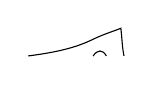
\begin{tikzpicture}[x=.8cm,y=.8cm]
\draw (0,0) .. controls (.46,.06) and (.75,.13) .. (1.02,.26)
  .. controls (1.18,.34) and (1.35,.39) .. (1.47,.44)
  .. controls (1.49,.28) and (1.49,.15) .. (1.52,0);
\draw (1.03,0) .. controls (1.10,.10) and (1.18,.11) .. (1.24,0);
\end{tikzpicture}}\endgroup\par
Угловая помета внизу слева. Штрихи обрываются на одной горизонтальной границе исходного кадра. Полная форма и назначение неясны.}
\end{GelfandAdjacentEvidence}



\Needspace{7\baselineskip}
\begin{GelfandAdjacentEvidence}{GELFAND-P000816}{1}
\SourcePage{GELFAND-P000816}{unlabelled}
\uuline{19/II-79г.}\qquad \uline{Сем. Гельфанда.}

\uuline{Белавин}.

\[
A_i(\theta),\qquad 1\le i\le M,\qquad\text{— символы}
\]
\(\theta\) — параметр

\uwave{Алгебра Замолодчикова}.

\begin{equation*}
A_i(\theta_1)A_\alpha(\theta_2)
=S_{ik}^{\alpha\beta}(\theta_1-\theta_2)A_\beta(\theta_2)A_k(\theta_1)\tag{1}
\end{equation*}
Требуется и ассоциативность. Тогда возникают кубические соотн.
\[
A_i(\theta_1)A_j(\theta_2)A_k(\theta_3)
\]
[Справа:] (своб. ассоц. алгебра, порожд. \(M\) континуумами перем. с соотн.)
\Unclear{GELFAND-P000816}{free-algebra-word}{В приписке читается «континуумами перем.».}
\end{GelfandAdjacentEvidence}
\begin{GelfandAdjacentEvidence}{GELFAND-P000816}{2}


Интерпретация (физическая)

\SourceFigure{GELFAND-P000816}{particle-motion}{%
\par\begingroup\color{black}\GelfandFitDiagram{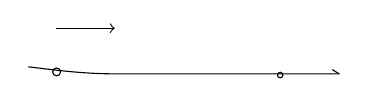
\begin{tikzpicture}[x=1cm,y=1cm]
\draw[->] (.35,.58) -- (1.10,.58);
\draw (0,.09) .. controls (.45,.035) and (.73,0) .. (1.15,0) -- (3.95,0);
\draw (3.86,.055) -- (3.95,0);
\draw (.36,.025) circle[radius=.05cm];
\draw (3.20,-.015) circle[radius=.035cm];
\end{tikzpicture}}\endgroup\par}
\end{GelfandAdjacentEvidence}
\begin{GelfandAdjacentEvidence}{GELFAND-P000816}{3}

полож. — частицы,\quad \(\theta_i\) — скорости
\Unclear{GELFAND-P000816}{particle-word}{Сокращение под рисунком предположительно читается как «полож.».}
\end{GelfandAdjacentEvidence}
\begin{GelfandAdjacentEvidence}{GELFAND-P000816}{4}


\(A_iA_\alpha\) — \(i\)-я част. левее.

\(\theta_1>\theta_2\ \Rightarrow\) догонит \(i\)-я.

Могут догонять по разному, но важны начало и конец
(что в промежутке — не важно)

\SourceFigure{GELFAND-P000816}{collision-diagrams}{%
\par\begingroup\color{black}\GelfandFitDiagram{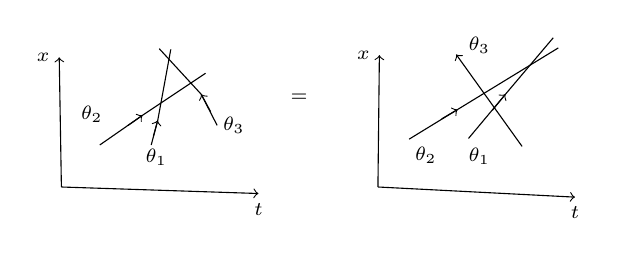
\begin{tikzpicture}[x=.92cm,y=.92cm,every node/.style={font=\scriptsize}]
\draw[->] (0,0) -- (2.72,-.09) node[below] {\(t\)};
\draw[->] (0,0) -- (-.03,1.79) node[left] {\(x\)};
\draw (.53,.58) -- (1.12,.99) -- (1.99,1.57);
\draw[->] (.92,.85) -- (1.12,.99);
\draw (1.24,.58) -- (1.33,.92) -- (1.51,1.90);
\draw[->] (1.27,.70) -- (1.33,.92);
\draw (2.15,.85) -- (1.93,1.28) -- (1.35,1.91);
\draw[->] (2.06,1.04) -- (1.93,1.28);
\node at (.42,1) {\(\theta_2\)};
\node at (1.31,.41) {\(\theta_1\)};
\node at (2.38,.85) {\(\theta_3\)};
\node at (3.28,1.23) {\(=\)};
\begin{scope}[xshift=4.02cm]
\draw[->] (0,0) -- (2.72,-.14) node[below] {\(t\)};
\draw[->] (0,0) -- (.02,1.82) node[left] {\(x\)};
\draw (.43,.66) -- (1.10,1.07) -- (2.49,1.92);
\draw[->] (.88,.94) -- (1.10,1.07);
\draw (1.25,.67) -- (1.76,1.28) -- (2.42,2.06);
\draw[->] (1.58,1.06) -- (1.76,1.28);
\draw[->] (1.99,.56) -- (1.08,1.83);
\node at (.66,.44) {\(\theta_2\)};
\node at (1.40,.42) {\(\theta_1\)};
\node at (1.40,1.96) {\(\theta_3\)};
\end{scope}
\end{tikzpicture}}\endgroup\par
Наконечник на нисходящей линии \(\theta_3\) слева наведён. Направление передано предположительно вверх и влево.}
\end{GelfandAdjacentEvidence}
\begin{GelfandAdjacentEvidence}{GELFAND-P000816}{5}


\begin{align*}
&\bigl(A_i(\theta_1)A_j(\theta_2)\bigr)A_k(\theta_3)\\
&=S_{ii_1}^{jj_1}A_{j_1}(\theta_2)\bigl(A_{i_1}(\theta_1)A_k(\theta_3)\bigr)=\\
&=S_{ii_1}^{jj_1}(\theta_{12})S_{i_1i_2}^{kk_1}(\theta_{13})
   \bigl(A_{j_1}(\theta_2)A_{k_1}(\theta_3)\bigr)A_{i_2}(\theta_1)=\\
&=S_{ii_1}^{jj_1}(\theta_{12})S_{i_1i_2}^{kk_1}(\theta_{13})S_{j_1j_2}^{k_1k_2}(\theta_{23})\\
&\qquad A_{k_2}(\theta_3)A_{j_2}(\theta_2)A_i(\theta)
\end{align*}
\Unclear{GELFAND-P000816}{chain-first-aj}{В первом произведении буква \(A\) у \(A_j(\theta_2)\) наведена. Первоначальный штрих не читается.}
\end{GelfandAdjacentEvidence}
\begin{GelfandAdjacentEvidence}{GELFAND-P000816}{6}


\Unclear{GELFAND-P000816}{chain-first-s}{У \(S_{ii_1}^{jj_1}\) в первом равенстве аргумент не написан.}
\end{GelfandAdjacentEvidence}
\begin{GelfandAdjacentEvidence}{GELFAND-P000816}{7}


\Unclear{GELFAND-P000816}{chain-reworked-theta}{В последнем произведении у \(A_{k_2}\) знак \(\theta\) в \(\theta_3\) наведён. Первоначальный штрих не читается.}
\end{GelfandAdjacentEvidence}
\begin{GelfandAdjacentEvidence}{GELFAND-P000816}{8}


\Unclear{GELFAND-P000816}{chain-last-factor}{Последний множитель записан как \(A_i(\theta)\) без дополнительных цифровых индексов.}
\end{GelfandAdjacentEvidence}



\Needspace{7\baselineskip}
\begin{GelfandAdjacentEvidence}{GELFAND-P000817}{1}
\SourcePage{GELFAND-P000817}{67}
\uline{Ур-я приобр. вид}:
\begin{equation*}
\begin{aligned}
&S^{kk_1}_{ii_1}(\theta)S^{jj_1}_{i_1i_2}(\theta+\theta')
  S^{j_1j_2}_{k_1k_2}(\theta')\\
&=S^{jj_1}_{kk_1}(\theta')S^{j_1j_2}_{ii_1}(\theta+\theta')
  S^{k_1k_2}_{i_1i_2}
\end{aligned}\tag{2}
\end{equation*}
\Unclear{GELFAND-P000817}{eq2-index-arguments}{Индексы в (2) набраны по рукописи. У последнего \(S\) аргумент не написан.}
\end{GelfandAdjacentEvidence}
\begin{GelfandAdjacentEvidence}{GELFAND-P000817}{2}


По \(i_1,j_1,k_1\) суммир.

Итого: \(M^6\) ур-й на \(M^4\) ф-й \(S^{\alpha\beta}_{ik}(\theta)\)

\(S\) играет роль \(S\)-матрицы.

Положим
\begin{equation*}
T_{\vec{\alpha},\vec{\beta}}(\theta)=
S^{\alpha_1\beta_1}_{i_1i_2}(\theta)
S^{\alpha_2\beta_2}_{i_2i_3}(\theta)
\cdot\;\cdot\;\cdot\;\cdot
S^{\alpha_N\beta_N}_{i_Ni_1}(\theta)\tag{3}
\end{equation*}
\Unclear{GELFAND-P000817}{eq3-middle-subscript}{Нижние индексы среднего множителя наведены и читаются предположительно как \(i_2i_3\).}
\end{GelfandAdjacentEvidence}
\begin{GelfandAdjacentEvidence}{GELFAND-P000817}{3}


\Unclear{GELFAND-P000817}{eq3-final-subscript}{Нижние индексы последнего множителя наведены и читаются предположительно как \(i_Ni_1\), возможно \(i_Nk_1\).}
\end{GelfandAdjacentEvidence}
\begin{GelfandAdjacentEvidence}{GELFAND-P000817}{4}


Получится матрица \(M^N\times M^N\)
(«трансфер-матрица»)

[Справа:] \((\alpha_1,\ldots,\alpha_N)\) — индексы.

\((\beta_1,\ldots,\beta_N)\) — 2-й набор инд.

Утверждается, что
\begin{equation*}
[T(\theta),T(\theta')]=0\tag{4}
\end{equation*}
[Справа от нуля зачёркнуто: \(\ldots\)]
\Incomplete{GELFAND-P000817}{eq4-crossed-right}{запись неразборчива}
\end{GelfandAdjacentEvidence}
\begin{GelfandAdjacentEvidence}{GELFAND-P000817}{5}


(в силу ур-й факторизации).

[Слева зачёркнута подчёркнутая запись: \(\ldots\)]
\Incomplete{GELFAND-P000817}{eq4-crossed-left}{запись неразборчива}
\end{GelfandAdjacentEvidence}
\begin{GelfandAdjacentEvidence}{GELFAND-P000817}{6}


Факториз. \(S\)-матр. — следствие кон. числа законов сохр.

\uline{Явная запись ур-й при \(M=2\)}

(случай ур-й Максвелла)
\begin{equation*}
\begin{cases}
A_1A_1=a\,A_1A_1+d\,A_2A_2\\
A_1A_2=b\,A_2A_1+c\,A_1A_2
\end{cases}
\qquad
\begin{pmatrix}
A_1(\theta_1),\ A_2(\theta_2)\\
a(\theta_1-\theta_2)
\end{pmatrix}\tag{5}
\end{equation*}
[Справа:] и ещё 2 ур-я с заменой 1 на 2
(с теми же коэфф.)
(см. \((5)_2\))

Есть 4 ф-й \(a,b,c,d\).

Могли бы быть 16 ф-й. На самом деле 5 или 6 ф-й (из ур-й).

Здесь оставлено 4 штуки

\uwave{Ур-я факторизации дают}:
\begin{equation*}
\left\{
\begin{aligned}
a(\theta)a(\theta+\theta')d(\theta')
&=d(\theta+\theta')a(\theta')\\
&\quad +b(\theta)b(\theta+\theta')d(\theta')
\end{aligned}
\right.\tag{6}
\end{equation*}
\SourceFigure{GELFAND-P000817}{eq6-dashed-row}{%
\par\begingroup\color{black}\GelfandFitDiagram{\begin{tikzpicture}[x=.004cm,y=.004cm]
\foreach \pos/\height/\len in {71/27/14,193/24/32,321/21/18,421/22/22,550/23/26,705/22/27,836/14/38,973/6/35,1075/2/28,1173/1/37,1289/3/41,1430/2/65,1556/4/40}
  \draw (\pos,\height) -- ++(\len,0);
\end{tikzpicture}}\endgroup\par
Ряд коротких штрихов под выписанной строкой (6).}
\end{GelfandAdjacentEvidence}
\begin{GelfandAdjacentEvidence}{GELFAND-P000817}{7}


Здесь положено \(c(\theta)\equiv1\) (ур-я однородные — поделим).
\Unclear{GELFAND-P000817}{eq6-verb}{Глагол читается как «положено», возможно «положим».}
\end{GelfandAdjacentEvidence}
\begin{GelfandAdjacentEvidence}{GELFAND-P000817}{8}


[Справа:] (всего 6 функц. ур-й)

\begin{equation*}
\begin{cases}
A_2A_2=a\,A_2A_2+d\,A_1A_1\\
A_2A_1=b\,A_1A_2+c\,A_2A_1
\end{cases}\tag*{\((5)_2\)}
\end{equation*}
\Unclear{GELFAND-P000817}{eq5-repeat-label}{Под наведённой цифрой 5 в \((5)_2\) первоначальный знак не читается.}
\end{GelfandAdjacentEvidence}
\begin{GelfandAdjacentEvidence}{GELFAND-P000817}{9}


\begin{equation*}
S^{\alpha\beta}_{ik}(0)=\delta_{i\beta}\delta_{\alpha k}\tag{7}
\end{equation*}
— \uline{нач. условие}

\uwave{Получим из (6) дифф. ур-я}:
\begin{equation*}
\left\{
\begin{aligned}
\dot a&=\alpha a-\beta b+\gamma ad\\
\dot d&=\alpha d+\gamma(a^2-b^2)\\
a\dot b-b\dot a&=\beta(1-d^2)\\
d\dot b-b\dot d&=\alpha bd+\gamma b-\beta ad\\
&\text{и ещё 2 ур-я.}
\end{aligned}
\right.
\qquad
\begin{aligned}
\dot a(0)&=\alpha\\
\dot b(0)&=\beta\\
\dot d(0)&=\gamma
\end{aligned}\tag{8}
\end{equation*}
\Unclear{GELFAND-P000817}{eq8-overwrite}{В третьей строке (8) \(b\dot a\) наведено. Первоначальные штрихи не читаются.}
\end{GelfandAdjacentEvidence}



\Needspace{7\baselineskip}
\begin{GelfandAdjacentEvidence}{GELFAND-P000818}{1}
\SourcePage{GELFAND-P000818}{unlabelled}
Все ур-я независимы.

Возник. 3 алгебр. соотношения, но одно — следствие 2-х других.

Получаются эллиптич. ф-и (Бакстер)

Возникает некоммут., не ассоц. алгебра четверок ф-й.
\Unclear{GELFAND-P000818}{top-quadruples}{Слово читается «четверок». Штрихи над «е» могут обозначать «ё».}
\end{GelfandAdjacentEvidence}
\begin{GelfandAdjacentEvidence}{GELFAND-P000818}{2}


Интересно найти явную \uline{реализ.} (напр., на матрицах)

\uwave{Идея Ю. И. Манина}: взять \uline{точки} \uline{на} элл. кривой конечного порядка

Разложим
\begin{equation*}
T(\theta)=\sum_{\ell=0}^{\infty}I_{\ell}\theta^{\ell}\tag{9}
\end{equation*}
Тогда
\begin{equation*}
[I_n,I_m]=0\tag{10}
\end{equation*}
и в примере (\(M=2\)):
\begin{equation*}
\text{\uwave{\mbox{\(\displaystyle I_0^{-1}\,\text{\sout{(0)}}\,I_1\)}}}\,
\text{\sout{(0)}}
=\sum_{n=1}^{N}\sum_{\alpha=1}^{3}J_\alpha\sigma_n^\alpha\sigma_{n+1}^\alpha
\quad(=T^{-1}(0)\dot T(0))=H\tag{11}
\end{equation*}
\Unclear{GELFAND-P000818}{eq11-crossing-01}{После \(I_0^{-1}\) зачёркнута запись, возможно \((0)\).}
\end{GelfandAdjacentEvidence}
\begin{GelfandAdjacentEvidence}{GELFAND-P000818}{3}


\Unclear{GELFAND-P000818}{eq11-crossing-02}{После \(I_1\) зачёркнута отдельная запись, также возможно \((0)\).}
\end{GelfandAdjacentEvidence}
\begin{GelfandAdjacentEvidence}{GELFAND-P000818}{4}


Здесь
\[
\sigma_n^\alpha=1\otimes\ldots\otimes\sigma^\alpha\otimes\ldots\otimes1,
\qquad\sigma^\alpha\text{ — матрицы Паули.}
\]
\begin{equation*}
[I_\ell,H]=0,\quad\ell=0,1,2,\ldots\tag{12}
\end{equation*}
Трансфер-матр пишется через \(S\), т. е. через эллипт. ф-и.

\(I_2\) сод. 3 спина и т. д.

\uline{И. М. Г.}\quad \(a,b,c,d\) — наверное, \(SL(2,R)\)
\Unclear{GELFAND-P000818}{middle-maybe}{Слово предположительно читается «наверное», возможно «наверно».}
\end{GelfandAdjacentEvidence}
\begin{GelfandAdjacentEvidence}{GELFAND-P000818}{5}


\(d=0\Rightarrow\) получ. обычные триг., а не эллипт. ф-и.

\SourceFigure{GELFAND-P000818}{middle-emphasis-strokes}{%
\par\begingroup\color{black}\GelfandFitDiagram{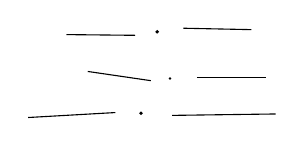
\begin{tikzpicture}[x=.9cm,y=.9cm]
\draw (.58,1.20)--(1.55,1.19);
\fill (1.86,1.24) circle[radius=.025cm];
\draw (2.23,1.29)--(3.19,1.27);
\draw (.88,.68)--(1.77,.55);
\fill (2.04,.58) circle[radius=.018cm];
\draw (2.42,.59)--(3.39,.59);
\draw (.04,.03)--(1.27,.10);
\fill (1.63,.09) circle[radius=.024cm];
\draw (2.07,.06)--(3.53,.08);
\end{tikzpicture}}\endgroup\par
Три ряда раздельных штрихов под записями о спинах, \(SL(2,R)\) и триг. ф-ях.}
\end{GelfandAdjacentEvidence}
\begin{GelfandAdjacentEvidence}{GELFAND-P000818}{6}


\uwave{Общее утверждение} (теперь \(M\) произвольно):

Положим
\begin{equation*}
\overset{\text{\sout{\(\ldots\)}}}{H}=
\sum_{n=1}^{N}\dot{S}_{ik}^{\alpha\beta}(0)\sigma_n^{i\beta}\sigma_{n+1}^{\alpha k}
=I_0^{-1}I_1
\qquad\text{(см. (9)).}\tag{13}
\end{equation*}
\Incomplete{GELFAND-P000818}{eq13-crossing-over-h}{Над \(H\) зачёркнут знак. Исходное начертание не читается.}
\end{GelfandAdjacentEvidence}
\begin{GelfandAdjacentEvidence}{GELFAND-P000818}{7}


\(\sigma\) — матрица \(M\times M\).
\SourceFigure{GELFAND-P000818}{matrix-unit-schematic}{%
\par\begingroup\color{black}\GelfandFitDiagram{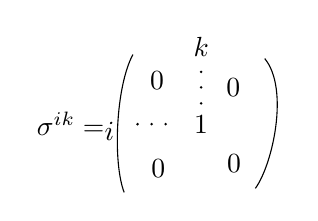
\begin{tikzpicture}[x=.85cm,y=.85cm]
\node at (-1.85,0) {\(\sigma^{ik}=\)};
\draw (-.92,1.04) .. controls (-1.18,.55) and (-1.22,-.58) .. (-1.05,-1.02);
\draw (1.05,.98) .. controls (1.42,.53) and (1.17,-.60) .. (.91,-.96);
\node at (-.56,.65) {\(0\)};
\node at (.58,.55) {\(0\)};
\node at (-.54,-.67) {\(0\)};
\node at (.59,-.59) {\(0\)};
\node at (.10,0) {\(1\)};
\foreach \x in {-.85,-.64,-.43} \fill (\x,0) circle[radius=.018cm];
\foreach \y in {.31,.55,.78} \fill (.10,\y) circle[radius=.018cm];
\node at (-1.27,-.11) {\(i\)};
\node at (.10,1.16) {\(k\)};
\end{tikzpicture}}\endgroup\par
базис в пр-ве матриц (\(1\) на месте \(i,k\)).}
\end{GelfandAdjacentEvidence}
\begin{GelfandAdjacentEvidence}{GELFAND-P000818}{8}

\[
\sigma_n^{ik}=1\otimes\ldots\otimes\underset{n}{\sigma^{ik}}\otimes\ldots\otimes1
\]
Имеем лок. гамильтониан.

\Unclear{GELFAND-P000818}{hamiltonian-abbrev}{Сокращение перед «гамильтониан» предположительно читается «лок.».}
\end{GelfandAdjacentEvidence}
\begin{GelfandAdjacentEvidence}{GELFAND-P000818}{9}


Замолодчиков получил \uwave{частные} решения (при разных \(M\))

Используем их при \(\underline{M=3}\), Получим
\begin{equation*}
H=\sum_n\text{\sout{\(\ldots\)}}(\vec{S}_n\,\vec{S}_{n+1})^2-2\vec{S}_n\,\vec{S}_{n+1}\tag{14}
\end{equation*}
\Incomplete{GELFAND-P000818}{eq14-crossing}{Между знаком суммы и открывающей скобкой запись перечёркнута. Исходные знаки не читаются.}
\end{GelfandAdjacentEvidence}


\(\underline{M=2}\) — изотр. ферромагн. Гейзенберга
\begin{equation*}
H=\sum_n\vec{\sigma}_n\,\vec{\sigma}_{n+1}\tag{15}
\end{equation*}
спин \(1/2\) — ничего больше инв. нет.


\Needspace{7\baselineskip}
\begin{GelfandAdjacentEvidence}{GELFAND-P000819}{1}
\SourcePage{GELFAND-P000819}{68}
В (14): \(S^\alpha\) такие, что
\begin{equation*}
[S^\alpha,S^\beta]=\varepsilon_{\alpha\beta\gamma}S^\gamma,\tag{16}
\end{equation*}
\(S^\alpha\) — беск. мал. поворот.
\Unclear{GELFAND-P000819}{upper-rotation-abbreviation}{Первое сокращение перед «мал. поворот» предположительно читается «беск.». Буквы местами перекрываются.}
\end{GelfandAdjacentEvidence}
\begin{GelfandAdjacentEvidence}{GELFAND-P000819}{2}


(предст. гр. \(SO(3)\))

присоед. \(=\) стандартное

Здесь нет параметров

\(\underline{\underline{M=3}}\Rightarrow\) общего реш. нет.

(!) \uwave{Неизвестно, как к гам. (14) добавить параметры, чтобы уложиться в сх. Замолодчикова.}

Эта схема сод. все вполне инт. квант. системы (2-мерные)

(\(\Rightarrow\) классические тоже после квазикласс. пред. перехода).

\begin{equation*}
H=\sum_{n=1}^{N}\dot S_{ik}^{\alpha\beta}(0)
 \sigma_n^{i\beta}\sigma_{n+1}^{\alpha k};\tag{17}
\end{equation*}
\uwave{Вопрос И.М.Г.}: соотн. на \(S\) — типа Маурера–Картана

(17) — наиболее общ. вид гам. с взаимод. ближ. соседей.

Он \uline{всегда} облад. нетрив. интегралом, т.к. дифф. ур-я прод. до 2-й окрестности.
\[
S=S(0)+S'(0)\theta+\frac{S''(0)\theta^2}{2}
\]
\(S''\) восстанавливается.

\(A_i(\theta)\) матрицы \(\Rightarrow\) есть \uwave{ассоциат.} автоматически

Сущ способ размножать алгебры.

Пусть нашли \(S_{ik}^{\alpha\beta}\). Построим

(напр. \(\underline{M=2}\))
\begin{equation*}
 L^{ik}_{\vec\alpha\vec\beta}
 =S_{ij_1}^{\alpha_1\beta_1}S_{j_2j_3}^{\alpha_2\beta_2}.\, .
 S_{j_Nk}^{\alpha_N\beta_N}
 \qquad\text{(след не взяли)}\tag{18}
\end{equation*}
\Unclear{GELFAND-P000819}{eq18-l-indices}{Начертание нижних индексов \(L\) передано как \(\vec\alpha\vec\beta\). Рядом видна зачёркнутая запись.}
\end{GelfandAdjacentEvidence}
\begin{GelfandAdjacentEvidence}{GELFAND-P000819}{3}


\Unclear{GELFAND-P000819}{eq18-product-indices}{Во втором множителе написаны нижние индексы \(j_2j_3\), хотя первый множитель оканчивается на \(j_1\). Между вторым и последним множителями две точки.}
\end{GelfandAdjacentEvidence}
\begin{GelfandAdjacentEvidence}{GELFAND-P000819}{4}


Получ. матрица
\begin{equation*}
L=\begin{pmatrix}L_{11}&L_{12}\\L_{21}&L_{22}\end{pmatrix}
=(L^{\alpha\beta})\tag{19}
\end{equation*}
элем. к-рой — \uline{тоже матрицы}.

[зачёркнуто: \sout{\(\ldots\)}]
Соотнош. типа (2) \(-\ -\) справедливы для матрицы \(L\)
\Incomplete{GELFAND-P000819}{lower-left-deletion}{Зачёркнутый знак перед «Соотнош.» не читается.}
\end{GelfandAdjacentEvidence}
\begin{GelfandAdjacentEvidence}{GELFAND-P000819}{5}


\begin{equation*}
S_{ik}^{\alpha\mu}S_{kj}^{\beta\nu}S_{\mu\gamma}^{\nu\delta}
=S_{\beta\nu}^{\alpha\mu}S_{ik}^{\mu\gamma}S_{kj}^{\nu\delta}
\tag*{(2)\('\)}
\end{equation*}
\(L^{ik}\) — матр. \(M^N\times M^N\) при всех \(i,k\).

Есть соотношения:
\begin{equation*}
\begin{array}{rccccccc}
 &L^{\alpha\mu}&L^{\beta\nu}&S_{\mu\gamma}^{\nu\delta}
 &=&S_{\beta\nu}^{\alpha\mu}&L^{\mu\gamma}&L^{\nu\delta}.\\
 \text{аргументы:}&\theta&\theta'&\theta-\theta'
 &&\theta-\theta'&\theta'&\theta
\end{array}\tag{20}
\end{equation*}
\Unclear{GELFAND-P000819}{eq20-argument-layout}{Аргументы приписаны под соответствующими множителями. Справа под двумя \(L\) стоят сначала \(\theta'\), затем \(\theta\).}
\end{GelfandAdjacentEvidence}



\Needspace{7\baselineskip}
\begin{GelfandAdjacentEvidence}{GELFAND-P000820}{1}
\SourcePage{GELFAND-P000820}{unlabelled}
Пусть теперь
\begin{equation*}
A_{\alpha\mu}=L^{\alpha\mu}\tag{21}
\end{equation*}
Получится новая алгебра более выс. порядка

\SourceFigure{GELFAND-P000820}{toroidal-grid}{%
\begingroup\color{black}\GelfandFitDiagram{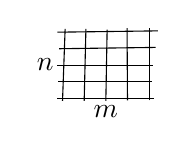
\begin{tikzpicture}[x=.55cm,y=.42cm]
\draw (-.12,0)--(2.12,0);
\draw (-.10,.5)--(2.06,.5);
\draw (-.12,1)--(2.10,1);
\draw (-.08,1.5)--(2.15,1.54);
\draw (-.12,2)--(2.20,2.04);
\draw (0,-.08)--(.06,2.1);
\draw (.5,-.08)--(.54,2.1);
\draw (1,-.08)--(1.03,2.08);
\draw (1.5,-.06)--(1.49,2.12);
\draw (2,-.06)--(2,2.12);
\node at (-.40,1.02) {\(n\)};
\node at (1,-.40) {\(m\)};
\end{tikzpicture}}\endgroup\par
2-мерн. решётка, свёрнутая в тор.}
\end{GelfandAdjacentEvidence}
\begin{GelfandAdjacentEvidence}{GELFAND-P000820}{2}


Онзагер в 44г. — 2-мерн. модель Изинга

\mbox{—\textbar\textbar—} 65г. — прид. коммут. трансфер-матрицу.
\Unclear{GELFAND-P000820}{onsager-verb}{Сокращение перед «коммут.» предположительно читается «прид.»; возможно «пред.».}
\end{GelfandAdjacentEvidence}
\begin{GelfandAdjacentEvidence}{GELFAND-P000820}{3}


\[
\sigma_{n,m}=\pm1
\]
Надо вычисл. сумму:
\begin{equation*}
Z=\sum_{\{\sigma_{n,m}\}}
e^{J_1\sum\sigma_{n,m}\sigma_{n,m+1}+J_2\sum\sigma_{n,m}\sigma_{n+1,m}\text{ \sout{…}}}
\tag{22}
\end{equation*}
\Incomplete{GELFAND-P000820}{exponent-cancellation}{Запись в конце показателя степени зачёркнута. Знаки не читаются.}
\end{GelfandAdjacentEvidence}
\begin{GelfandAdjacentEvidence}{GELFAND-P000820}{4}


(взаимод. ближ. соседей)

Идея:
\begin{equation*}
Z=\operatorname{Tr}T^N\tag{23}
\end{equation*}

\SourceFigure{GELFAND-P000820}{diagonal-dots}{%
\begingroup\color{black}\GelfandFitDiagram{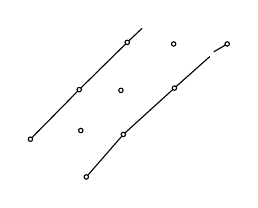
\begin{tikzpicture}[x=.010cm,y=.010cm]
\draw (27,59)--(89,122)--(150,182)--(169,200);
\draw (98,11)--(145,65)--(210,124)--(255,164);
\draw (260,170)--(277,180);
\foreach \x/\y in {27/59,89/122,150/182,91/70,142/121,209/180,98/11,145/65,210/124,277/180}
  \draw[fill=white] (\x,\y) circle[radius=.028cm];
\end{tikzpicture}}\endgroup\par
У верхнего кружка левой линии штрихи сливаются. Отдельный наконечник не различим.}
\end{GelfandAdjacentEvidence}
\begin{GelfandAdjacentEvidence}{GELFAND-P000820}{5}


[Справа:] \uwave{Онзагер}: идём по диагоналям (по спинам промежут. диаг. суммируем)
\begin{equation*}
T_{\vec\alpha\,\vec\beta}=S_1\ldots S_n,\tag{24}
\end{equation*}
где

\SourceFigure{GELFAND-P000820}{eq25-diamond}{%
\begingroup\color{black}\GelfandFitDiagram{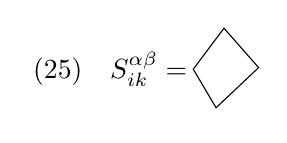
\begin{tikzpicture}[baseline=-.5ex]
\node[anchor=east,inner sep=2pt] at (0,.5) {\((25)\quad S_{ik}^{\alpha\beta}=\)};
\draw (0,.5)--(.39,1.02)--(.83,.52)--(.29,.01)--cycle;
\end{tikzpicture}}\endgroup}
\end{GelfandAdjacentEvidence}
\begin{GelfandAdjacentEvidence}{GELFAND-P000820}{6}


Получ. тр.-матр. \qquad \(T(J_1,J_2)\)

\uline{Утв.}

\(T(J_1,J_2)\) коммут. пр
\Incomplete{GELFAND-P000820}{bottom-fragment}{Последние видимые буквы «пр», возможно начало «при». Запись обрывается.}
\end{GelfandAdjacentEvidence}



\clearpage
\pdfbookmark[0]{Глава 15}{gelfand-archive-chapter-15}
\section*{Глава 15}
\Needspace{7\baselineskip}
\begin{GelfandAdjacentEvidence}{GELFAND-P000821}{1}
\SourcePage{GELFAND-P000821}{unlabelled}
[Вверху слева зачёркнуто: \sout{22…}]
\Unclear{GELFAND-P000821}{cancelled-page-label}{Начало зачёркнутой записи предположительно читается «22». Окончание не читается.}
\end{GelfandAdjacentEvidence}
\begin{GelfandAdjacentEvidence}{GELFAND-P000821}{2}


\uuline{26.2.79 г.} \qquad \uline{Сем. Гельфанда.}

\uuline{С. Гельфанд} \quad \uline{с лекции Манина}

Речь идёт о связи реш. Я.-М. с алг.-геом. объектами

(реш. не обяз. автодуальные)

— Виттен; незав. Яскин, Айзенберг, Грин (1978)
\Unclear{GELFAND-P000821}{researcher-names}{Фамилии в рукописи читаются «Яскин, Айзенберг, Грин».}
\end{GelfandAdjacentEvidence}
\begin{GelfandAdjacentEvidence}{GELFAND-P000821}{3}


\[
\widehat{\mathbb{C}M}=G(4,2)\qquad
\text{(грассманово мн-ие 2-мерных компл. плоскостей в \(\mathbb{C}^4\))}
\]
\Incomplete{GELFAND-P000821}{grassmannian-cancelled-index}{Справа внизу при \(G\) видна густо замазанная запись. Знак не читается.}
\end{GelfandAdjacentEvidence}
\begin{GelfandAdjacentEvidence}{GELFAND-P000821}{4}


[Под \(G(4,2)\):] (комп. грассманово мн-ие)

[Под формулой слева вертикальная черта к подписи:] комплексифицир. пр-во Минковского

(и компактифицир.)

(в \(G(4,2)\) есть открытое подмн-во, изом. \(\mathbb{C}^4\)).

\uwave{С. Гельфанд}

\(M^4\) (пр-во Минк.) с конф. метрикой компактифицир. т.е. свет. конуса

(на бесконечности). Все конф. преобр. тоже есть \(SU(2,2)\)

Получ. стац. группа \(SO(3,1)\)

\begin{equation*}
\widehat{M^4}=SU(2,2)/SO(3,1)\tag{1}
\end{equation*}
\Unclear{GELFAND-P000821}{minkowski-quotient}{В рукописи в знаменателе стоит \(SO(3,1)\).}
\end{GelfandAdjacentEvidence}
\begin{GelfandAdjacentEvidence}{GELFAND-P000821}{5}


Теперь скомплекс. \(SU(2,2)\) и \(SO(3,1)\) и берём фактор

\begin{equation*}
(SU(2,2)=SO(4,2))\tag{2}
\end{equation*}

\(SU(2,2)\) — конф. группа для \(M^4\)

\uwave{Геометрич. картинка.}

В \(\mathbb{C}P^3\) рассм. [зачёркнуто: \sout{конус}]
[вписано сверху: поверхность] (веществ. 5-мерный)
\Unclear{GELFAND-P000821}{surface-cancellation}{Отменённое слово предположительно читается «конус». Над ним написано «поверхность».}
\end{GelfandAdjacentEvidence}
\begin{GelfandAdjacentEvidence}{GELFAND-P000821}{6}


\begin{equation*}
R=\{z:|z_1|^2+|z_2|^2-|z_3|^2-|z_4|^2=0\}\subset\mathbb{C}P^3
\tag{3}
\end{equation*}

\SourceFigure{GELFAND-P000821}{projectivization-arrow}{%
\begingroup\color{black}\GelfandFitDiagram{\begin{tikzpicture}[baseline=(current bounding box.center)]
\node at (0,1.28) {или в};
\node (total) at (0,.80) {\(\mathbb{C}^4\backslash0\)};
\node (base) at (0,-.15) {\(\mathbb{C}P^3\)};
\node at (-.92,.29) {(4)};
\draw[->] (total)--(base);
\end{tikzpicture}}\endgroup\par
действует \(GL(4,\mathbb{C})\); пов. (3) сохр. группа \(SU(2,2)\)}
\end{GelfandAdjacentEvidence}
\begin{GelfandAdjacentEvidence}{GELFAND-P000821}{7}


\(G(4,2)\) — мн-ие прямых в \(\mathbb{C}P^3\);

(или 2-мерн. подпр-в в \(\mathbb{C}^4\))

На пов. (3) целиком лежит \uwave{мн-во прямых} вещ. размерности 4.

\(SU(2,2)\) переносится на это мн-во.

\uline{Теорема 1.} \uwave{Содерж. мн-ие этих прямых — пр-во Минковского.}
\Unclear{GELFAND-P000821}{theorem-opening-word}{Первое сокращение предположительно читается «Содерж.». Возможно «Соотв.».}
\end{GelfandAdjacentEvidence}
\begin{GelfandAdjacentEvidence}{GELFAND-P000821}{8}


[зачёркнуто: \sout{\uline{Доказ.}}]
\Unclear{GELFAND-P000821}{cancelled-proof-heading}{Зачёркнутый заголовок предположительно читается «Доказ.».}
\end{GelfandAdjacentEvidence}


Прямые на пов. (3) параметриз. унит. матрицами 2-го порядка
\[
(z_3,z_4)=U(z_1,z_2),\qquad U\in U(2)
\]

\uwave{Метрика Минковского.}

Рассм. фиксир. прямую \(L_0\) на \(R\). Рассм. все другие прямые на \(R\), к-рые её пересекают.
\uwave{Получ. 3-мерный конус} \(K_{L_0}\). Он сохр. при всех преобр., сохр. \(L_0\).
Получ. \(SO(3,1)\) и конус, наз. \uwave{световым}.

Точки пов. \(R\) можно интерпрет. как лучи света.

Можно собрать \uwave{все точки пересечений} \(L\subset R\) с \(L_0\).
Получается образующая конуса (световой).


\Needspace{7\baselineskip}
\begin{GelfandAdjacentEvidence}{GELFAND-P000822}{1}
\SourcePage{GELFAND-P000822}{2}
Ср.: кватернионный вариант (рассказывался когда-то).

Стац. подгруппа:
\[
GL(2,\mathbb{C})\times\mathbb{R}^3\qquad(?)
\]

Конф. группа получ. добавлением инверсии \(\frac{1}{\tau}\) (\(\tau\) — расст. Минковского)
к движениям (гр. \uline{Пуанкаре}).

\[
\begin{array}{@{}l@{}}
X=G(4,2)\\[-.3ex]
\cup\\[-.3ex]
\mathbb{C}^4\ni(z_1,z_2,z_3,z_4)
\end{array}
\]
\Unclear{GELFAND-P000822}{containment-mark}{Под \(X\) написан знак, похожий на \(\cup\). Он передан в том же вертикальном положении.}
\end{GelfandAdjacentEvidence}
\begin{GelfandAdjacentEvidence}{GELFAND-P000822}{2}


Там рассм. голом. связности, удовл. ур-ям Я.-М.

\(G\) — компл. гр. Ли; \(\mathfrak g\) — её алгебра Ли.

\((A_1(z),A_2(z),A_3(z),A_4(z))\) — голом. ф-и со знач. в \(\mathfrak g\)

(голом. в откр. области)

\begin{equation*}
F_{\mu\nu}(z)=\partial_\mu A_\nu-\partial_\nu A_\mu+[A_\mu,A_\nu],
\qquad \partial_\mu=\frac{\partial}{\partial z_\mu}.
\tag{5}
\end{equation*}

Форма связности:
\[
\omega=\sum A_\mu(z)\,dz_\mu
\]

\(F\) — форма кривизны этой связности (снова со знач. в алг. Ли)

\uwave{Ур-я Я.-М.}
\begin{equation*}
\sum_{\mu=1}^{4}\left\{\frac{\partial F_{\mu\nu}}{\partial z_\mu}
 +[F_{\mu\nu},A_\mu]\right\}=0,\qquad \nu=1,2,3,4.
\tag{6}
\end{equation*}
\Unclear{GELFAND-P000822}{yang-mills-commutator-order}{В (6) после плюса в рукописи стоит \([F_{\mu\nu},A_\mu]\).}
\end{GelfandAdjacentEvidence}
\begin{GelfandAdjacentEvidence}{GELFAND-P000822}{3}


\uwave{И.М.Г.} \quad Ландау: „лагранжиан — труп“ считал, что надо знать \(S\)-матрицу и всё.

Соотв. вещ. ур-я получ. из лагранжиана:

\begin{equation*}
L=\operatorname{tr}\int F_{\mu\nu}F^{\mu\nu}\,d^4x
\tag{7}
\end{equation*}

Решения (6) связаны с нек-рыми объектами компл. аналит. геометрии.

По \(\mathbb{C}^4\) строим
\[
\underset{\text{прямые в \(\mathbb{C}^4\)}}{\mathbb{C}P^3}
\qquad\text{и}\qquad
\underset{\text{гиперпл. в \(\mathbb{C}^4\)}}{\mathbb{C}P^3}
\]

[Перед формулой зачёркнуто: \sout{…}]
\Incomplete{GELFAND-P000822}{quadric-cancelled-sign}{Отдельный знак густо зачёркнут. Цифра не устанавливается.}
\end{GelfandAdjacentEvidence}
\begin{GelfandAdjacentEvidence}{GELFAND-P000822}{4}


\begin{equation*}
\mathbb{C}P^3\times\mathbb{C}P^3\supset
 Q=\{(\ell,\pi)\mid\ell\subset\pi\},\qquad \dim_{\mathbb{C}}G=5
\tag{8}
\end{equation*}
\Unclear{GELFAND-P000822}{dimension-glyph}{Буква после \(\dim_{\mathbb{C}}\) предположительно читается как \(G\); возможно \(Q\). У первого \(Q\) в этой строке верхняя петля замкнута.}
\end{GelfandAdjacentEvidence}
\begin{GelfandAdjacentEvidence}{GELFAND-P000822}{5}


[Вертикальная черта вниз от \(Q\):] мн-ие, зад. двойственность (неполные ф-лаги)
\Unclear{GELFAND-P000822}{quadric-caption-word}{Сокращение перед «двойственность» условно передано «зад.». Начальный нисходящий штрих и последняя петля допускают иное чтение.}
\end{GelfandAdjacentEvidence}
\begin{GelfandAdjacentEvidence}{GELFAND-P000822}{6}


\uwave{2-й объект}.

(9) \uwave{Голоморфные расслоения на} \(Q\) \uwave{со структурной группой} \(G\), \uwave{к-рые}
\uwave{голом. продолжаются на 3-ю инфинитезим. окрестность} \(Q\) в \(\mathbb{C}P^3\times\mathbb{C}P^3\).

(На самом деле всё над подмножествами).
\Unclear{GELFAND-P000822}{subset-word-overwriting}{В слове «подмножествами» несколько букв исправлены. Предыдущее начертание не читается.}
\end{GelfandAdjacentEvidence}


Все связности \(\Longleftrightarrow\) все расслоения (не обязательно продолжающиеся на 3-ю инфинит. окрестность)


\Needspace{7\baselineskip}
\begin{GelfandAdjacentEvidence}{GELFAND-P000823}{1}
\SourcePage{GELFAND-P000823}{unlabelled}
\uline{А. Бейлинсон}

на \(G(4,2)\) рассм. полн. пр-во флагов \(F\) (прямая, плоскость, гиперпл.)

\SourceFigure{GELFAND-P000823}{left-margin-sketches}{%
\begingroup\color{black}\GelfandFitDiagram{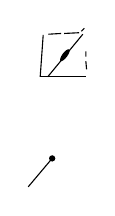
\begin{tikzpicture}[x=.95cm,y=.95cm]
\draw (-.14,.15)--(-.10,.71);
\draw (-.14,.15)--(.47,.15);
\draw (-.03,.72)--(.14,.73) (.18,.73)--(.38,.74) (.41,.76)--(.45,.80);
\draw (.48,.25)--(.47,.36) (.47,.42)--(.47,.49);
\draw (-.04,.15)--(.43,.72);
\fill[rotate around={53:(.19,.44)}] (.19,.44) ellipse[x radius=.092cm,y radius=.032cm];
\draw (-.30,-1.32)--(.02,-.94);
\fill (.02,-.94) circle[radius=.04cm];
\end{tikzpicture}}\endgroup\par
Верхний и правый края прерывисты. На наклонных чертах видны утолщения.}
\end{GelfandAdjacentEvidence}
\begin{GelfandAdjacentEvidence}{GELFAND-P000823}{2}


\SourceFigure{GELFAND-P000823}{flag-projections}{%
\begingroup\color{black}\GelfandFitDiagram{\begin{tikzpicture}[x=.84cm,y=.76cm,every node/.style={inner sep=1pt}]
\node (lf) at (0,0) {\(F\)};
\node (lg) at (0,-1.1) {\(G(4,2)\)};
\draw[->] (lf)--(lg);
\node[font=\scriptsize,anchor=west] at (.22,-.48) {— \uwave{забываем крайние}};
\begin{scope}[xshift=1.48cm]
\node (rf) at (3.07,0) {\(F\)};
\node (rq) at (3.07,-1.1) {\(Q\)};
\draw[->] (rf)--(rq);
\node at (3.49,-1.1) {\(\hookrightarrow\)};
\node at (4,-1.1) {\(P^3\)};
\node at (4.32,-1.1) {\(\times\)};
\node at (4.81,-1.1) {\(P^{3*}\)};
\draw (3.94,-1.35)--(3.83,-1.63) (4.79,-1.35)--(4.93,-1.62);
\node[font=\scriptsize] at (3.53,-1.85) {точки};
\node[font=\scriptsize] at (5.20,-1.85) {гиперпл.};
\end{scope}
\end{tikzpicture}}\endgroup\par
В правой схеме от \(Q\) вправо идёт крюкообразная стрелка.}
\end{GelfandAdjacentEvidence}
\begin{GelfandAdjacentEvidence}{GELFAND-P000823}{3}


[Справа от правого \(F\) зачёркнуто: \sout{…}]
\Incomplete{GELFAND-P000823}{cancelled-right-projection}{Вертикальная запись закрыта штрихами. Исходный знак не читается.}
\end{GelfandAdjacentEvidence}
\begin{GelfandAdjacentEvidence}{GELFAND-P000823}{4}


\SourceFigure{GELFAND-P000823}{point-hyperplane-sketches}{%
\begingroup\color{black}\GelfandFitDiagram{\begin{tikzpicture}[x=1cm,y=1cm]
\draw (0,0)--(.14,.57) (.17,.59)--(.85,.72) (0,0)--(.86,.20);
\draw (.86,.25)--(.86,.38) (.87,.56)--(.87,.60);
\fill (.32,.42) circle[radius=.046cm];
\fill (1.74,.81) circle[radius=.039cm];
\draw (3.11,.45)--(3.17,.84) (3.19,.89)--(3.77,.93) (3.11,.45)--(3.77,.46);
\draw (3.74,.54)--(3.78,.69) (3.79,.75)--(3.82,.82);
\draw (3.90,.95)--(4.03,1.09);
\end{tikzpicture}}\endgroup\par
Между двумя фигурами отдельная точка. Вверху справа короткий штрих, связь с контуром неясна.}
\end{GelfandAdjacentEvidence}
\begin{GelfandAdjacentEvidence}{GELFAND-P000823}{5}


\[
\begin{gathered}
(E,\nabla)\\
\text{рассл. со связностью}\\
\text{на }G(4,2)
\end{gathered}
\]

\uwave{Слой правого рассл. изом.} \(\mathbb{C}P^1\)

При левой проекции он перех. в \(\mathbb{C}P^1\)

на \(\mathbb{C}P^1\) рассл. тривиализуется (канонически), т.к. кривизна \(=0\) ввиду одномерности

(фунд. группа \(=0\)).

Связность (\(\omega\)) поднимаем на \(F\) и пытаемся спустить на \(Q\).
\Unclear{GELFAND-P000823}{connection-parenthesis}{Знак в скобках предположительно читается \(\omega\). Здесь его начертание отличается от \(\nabla\) в паре \((E,\nabla)\).}
\end{GelfandAdjacentEvidence}
\begin{GelfandAdjacentEvidence}{GELFAND-P000823}{6}


[Под строкой] (с \(G(4,2)\))

Она на \(\forall\) слое тривиальна \(\Rightarrow\) может быть передана на \(Q\)

Получ. \(\widetilde E\) — голом. вект. расслоение на \(Q\)
\Unclear{GELFAND-P000823}{bundle-accent}{Над первым \(E\) видна толстая, почти горизонтальная черта. Ниже волнистый знак выражен отчётливее.}
\end{GelfandAdjacentEvidence}
\begin{GelfandAdjacentEvidence}{GELFAND-P000823}{7}


\SourceFigure{GELFAND-P000823}{lower-notation}{%
\((E,\nabla)\longleftrightarrow\widetilde E\)\par
\(\widetilde E\) трив. на \(\mathbb{C}P^1\times\mathbb{C}P^1\)\par
\begingroup\color{black}\GelfandFitDiagram{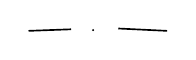
\begin{tikzpicture}
\draw[semithick] (0,0)--(.54,.02) (1.14,.03)--(1.76,0);
\fill (.82,.01) circle[radius=.014cm];
\end{tikzpicture}}\endgroup\par
Под последней строкой две черты с точкой между ними.}
\end{GelfandAdjacentEvidence}



\Needspace{7\baselineskip}
\begin{GelfandAdjacentEvidence}{GELFAND-P000824}{1}
\SourcePage{GELFAND-P000824}{unlabelled}
\uuline{5/III-79} \qquad \uline{Сем. Гельфанда}

\uuline{Д. Б. Фукс.}

\uuline{О \(\infty\)-мерных алгебрах Ли}

(построение и классификация).

\uwave{Градуир. алг. Ли}:
\[
\mathfrak g=\bigoplus_{i\in\mathbb{Z}}\mathfrak g_i,\qquad
[\mathfrak g_i,\mathfrak g_j]\subset\mathfrak g_{i+j}
\]
отсюда \(\mathfrak g_0\) — подалг., а все \(\mathfrak g_i\) —
\(\mathfrak g_0\)-модули.

\uwave{Картановская конструкция}:
\begin{equation*}
\mathfrak g_i=0\quad\text{при }i<i_0.\tag{1}
\end{equation*}
\uwave{Транзитивность}: имеется гомом.
\begin{equation*}
\mathfrak g_i\to\operatorname{Hom}(\mathfrak g_{-1},\mathfrak g_{i-1})\tag{2}
\end{equation*}
\begin{equation*}
\mathfrak g_i\to\operatorname{Hom}(\mathfrak g_1,\mathfrak g_{i+1})\tag{3}
\end{equation*}
\begin{equation*}
\left\{\begin{aligned}
i\ge0&\ \Rightarrow\ (2)\ \text{мономорфно}\\
i\le0&\ \Rightarrow\ (3)\ \text{мономорфно}
\end{aligned}\right.\tag{4}
\end{equation*}
Тогда есть теор. Картана о классификации: есть 4 серии.

1) \(W_n\) — полиномиальные вект. поля на \(\mathbb{C}^n\):
\begin{equation*}
\sum p_i(x_1,\ldots,x_n)\frac{\partial}{\partial x_i}\tag{5}
\end{equation*}
\(\deg\frac{\partial}{\partial x_i}=-1,\)
[зачёркнуто: \sout{…}]
\(\deg x_i=1.\)
\Incomplete{GELFAND-P000824}{degree-cancel}{Между двумя степенями зачёркнут знак. Исходное начертание не читается.}
\end{GelfandAdjacentEvidence}
\begin{GelfandAdjacentEvidence}{GELFAND-P000824}{2}


Здесь

\(\mathfrak g_0\) — \uwave{алг. матриц}(!)
(порожд. полями \(x_j\frac{\partial}{\partial x_i}\)).

2) бездиверг. вект. поля \(S_n\)
\Unclear{GELFAND-P000824}{divergence-series-mark}{У правого верхнего края \(S\) есть короткий восходящий штрих, соединённый с буквой. Возможно, это её окончание или знак штриха.}
\end{GelfandAdjacentEvidence}


3) гамильтоновы \(H_n\)

4) контактные \(K_n\) \qquad сохр. конт. стр. в \(\mathbb{C}^{2n+1}\)

(описание градуир. опускается)

(все — полиномиальные)

\uline{Идея док-ва}:

карт. продолжение.

Для простоты считаем \(i_0=-1\) (в (1))
\begin{equation*}
\mathfrak g=\mathfrak g_{-1}\oplus\mathfrak g_0\oplus\cdots\tag{6}
\end{equation*}
По \(\mathfrak g_0\) и \(\mathfrak g_{-1}\) всё восстанавливается


\Needspace{7\baselineskip}
\begin{GelfandAdjacentEvidence}{GELFAND-P000825}{1}
\SourcePage{GELFAND-P000825}{10}
Имеем:
\begin{equation*}
\mathfrak g_1\subset\operatorname{Hom}(\mathfrak g_{-1},\mathfrak g_0)\tag{7}
\end{equation*}
\[
\begin{gathered}
f\in\operatorname{Hom}(\mathfrak g_{-1},\mathfrak g_0),\quad
\alpha_1,\alpha_2\in\mathfrak g_{-1}\quad\Rightarrow\\
\Rightarrow
\end{gathered}
\]
\begin{equation*}
f(\alpha_1)\alpha_2=f(\alpha_2)\alpha_1\tag{8}
\end{equation*}
(из тожд. Якоби)
\Unclear{GELFAND-P000825}{eq8-retraced-index}{Индекс у второго \(\alpha\) в левой части наведён. Видимое начертание читается как 2.}
\end{GelfandAdjacentEvidence}
\begin{GelfandAdjacentEvidence}{GELFAND-P000825}{2}


Пусть
\begin{equation*}
\mathfrak g_1=\{f\in\operatorname{Hom}(\mathfrak g_{-1},\mathfrak g_0)
\mid f(\alpha_1)\alpha_2=f(\alpha_2)\alpha_1\}\tag{9}
\end{equation*}
\begin{equation*}
\begin{aligned}
\mathfrak g_2 &\subset\operatorname{Hom}(\mathfrak g_{-1},\mathfrak g_1)
\subset\operatorname{Hom}(\mathfrak g_{-1},\operatorname{Hom}(\mathfrak g_{-1},\mathfrak g_0))=\\
&=\operatorname{Hom}(\mathfrak g_{-1}\otimes\mathfrak g_{-1},\mathfrak g_0)
\end{aligned}\tag{10}
\end{equation*}
Тожд. Якоби \(\Rightarrow\)
\begin{equation*}
f(\alpha_1\otimes\alpha_2)\alpha_3\text{ — симм. по всем 3-м перем.}\tag{11}
\end{equation*}
Положим
\begin{equation*}
\mathfrak g_2=\left\{\begin{aligned}
&f\in\operatorname{Hom}(\mathfrak g_{-1}\otimes\mathfrak g_{-1},\mathfrak g_0)\mid\\
&f(\alpha_1\otimes\alpha_2)\alpha_3\text{ симм. по всем пер.}
\end{aligned}\right\}\tag{12}
\end{equation*}
и далее
\begin{equation*}
\mathfrak g_k=\left\{\begin{aligned}
&f\in\operatorname{Hom}(\overset{k}{\bigotimes}\mathfrak g_{-1},\mathfrak g_0)\mid\\
&f(\alpha_1\otimes\cdots\otimes\alpha_k)\alpha_{k+1}\text{ симметрично}
\end{aligned}\right\}\tag{13}
\end{equation*}
Коммутатор в \(\bigl[\bigoplus \mathfrak g_k\bigr]\) — ?

с \(\mathfrak g_{-1}\) коммут. определён уже, с \(\mathfrak g_0\) — тоже.
\[
\alpha\in\mathfrak g_k,\quad \beta\in\mathfrak g_\ell\quad\Rightarrow\quad
\text{для опр. }[\alpha,\beta]\text{ нужно задать}
\]
\[
[[\alpha,\beta],\delta],\qquad\delta\in\mathfrak g_{-1}
\]
\Unclear{GELFAND-P000825}{bracket-letter}{Одинаковая буква в обоих местах предположительно читается \(\delta\). Возможна \(\gamma\).}
\end{GelfandAdjacentEvidence}
\begin{GelfandAdjacentEvidence}{GELFAND-P000825}{3}


Тожд. Якоби \(\rightsquigarrow\) в члены, опр. по индукции.

[Зачёркнуто: \sout{Надо, чтобы \(\mathfrak g_0\) и \(\mathfrak g_{-1}\) были …}]
\Unclear{GELFAND-P000825}{cancel-prefix}{Начало зачёркнутой строки дано предположительно. Связка между двумя \(\mathfrak g\) и знак перед индексом 1 пересечены штрихами.}
\end{GelfandAdjacentEvidence}
\begin{GelfandAdjacentEvidence}{GELFAND-P000825}{4}


\Incomplete{GELFAND-P000825}{cancel-ending}{Окончание зачёркнутой строки не читается.}
\end{GelfandAdjacentEvidence}


\(\mathfrak g_0,\mathfrak g_{-1}\) могут быть любыми. Простота — доп. условие.

Но: как правило, получ. конечномерная алгебра!!

\(\infty\)-мерность — \uline{везение}.

\uline{Другая констр.}

Пусть \(\mathfrak g_{-1},\mathfrak g_0\) заданы,\qquad
\(\mathfrak g_0\subset\operatorname{End}(\mathfrak g_{-1})\).


\Needspace{7\baselineskip}
\begin{GelfandAdjacentEvidence}{GELFAND-P000826}{1}
\SourcePage{GELFAND-P000829}{12}
\uline{2-я констр.} \quad Пусть

Есть инволюция в \(\mathfrak g\): \(\tau:\mathfrak g\to\mathfrak g\). Тогда

\SourceFigure{GELFAND-P000829}{eigenspace-callouts}{%
\begingroup\color{black}\GelfandFitDiagram{\begin{tikzpicture}[every node/.style={inner sep=1pt}]
\node at (0,0) {\(\mathfrak g=\)};
\node (plus) at (.72,0) {\(\mathfrak g_+\)};
\node at (1.18,0) {\(\oplus\)};
\node (minus) at (1.66,0) {\(\mathfrak g_-\)};
\node[anchor=north] at (.72,-.58) {подалг.};
\node[anchor=north west] at (1.65,-.75) {\(\mathfrak g_+\)-модуль.};
\draw (plus.south)--(.72,-.48) (minus.south)--(1.72,-.56);
\end{tikzpicture}}\endgroup}
\end{GelfandAdjacentEvidence}
\begin{GelfandAdjacentEvidence}{GELFAND-P000829}{2}


Алгебра — подалгебра \(\mathfrak g\otimes\mathbb{C}[t,t^{-1}]\)

вида
\[
\ldots\oplus\mathfrak g_-t^{-1}\oplus\mathfrak g_+
\oplus\mathfrak g_-t\oplus\mathfrak g_+t^2\oplus\ldots
\]

\(\mathfrak g=sl(3),\qquad\tau:\) отр. отн. диаг. (\(-\)транспонир.)

[Зачёркнуто: \sout{\uwave{Другие алгебры}}]
\Unclear{GELFAND-P000829}{cancelled-heading}{Под чертами предположительно читается «Другие алгебры». Заголовок волнисто подчёркнут.}
\end{GelfandAdjacentEvidence}
\begin{GelfandAdjacentEvidence}{GELFAND-P000829}{3}


[Слева зачёркнуто: \sout{\(\mathfrak g\)}]
\Unclear{GELFAND-P000829}{cancelled-letter}{Под перечёркиванием видна нижняя петля. Знак похож на \(\mathfrak g\).}
\end{GelfandAdjacentEvidence}


\uwave{Другие алгебры Ли.}

порожд. \(\varepsilon_i,\ i\in\mathbb{Z},\quad
[\varepsilon_i,\varepsilon_j]=a_{ij}\varepsilon_{i+j}\)

есть 3 простых

\uline{1-я}:
\[
a_{ij}=\left\{\begin{aligned}
 &1,0,-1\\
 &\equiv j-i\quad\mathrm{mod}\,3
\end{aligned}\right.
\]

\uwave{Эти 2 констр. исчерпывают всё с точн. до градуировки.}


\Needspace{7\baselineskip}
\begin{GelfandAdjacentEvidence}{GELFAND-P000830}{1}
\SourcePage{GELFAND-P000830}{unlabelled}
\uuline{19/III - 79 г.} \qquad \uline{Сем. Гельфанда.}

\uuline{Огиевецкий} (Виктор Исаакович)

\uline{Супергравитация}

(\(=\) гравитация \(+\) суперсимметрия)

\(P_m,\ L_{mn}\) — генераторы гр. Пуанкаре

[Справа:]
\[
\begin{array}{@{}lr@{}}
P_m&\text{— 4 штуки}\\
L_{mn}&\text{— 6 штук}\\ \hline
\text{итого}&\text{10 штук}
\end{array}
\]

\(Q_\alpha,\overline{Q}_\alpha\) — спинорные генераторы
\[
\alpha=1,2
\]
\Unclear{GELFAND-P000830}{spinor-overwrite}{Начальные буквы слова «спинорные» наведены. Прежние штрихи не читаются.}
\end{GelfandAdjacentEvidence}
\begin{GelfandAdjacentEvidence}{GELFAND-P000830}{2}


\begin{equation*}
\{Q_\alpha,\overline{Q}_{\dot\alpha}\}
=2\sigma^m_{\alpha\dot\alpha}P_m;\tag{1}
\end{equation*}

\[
P_m=\sigma^m_{\alpha\dot\beta}P_{\alpha\dot\beta}
\]
\Unclear{GELFAND-P000830}{vector-indices}{Верхний индекс у \(\sigma\) предположительно \(m\), возможно \(n\). Короткий штрих над \(\alpha\) второго \(P\) похож на отделившийся верхний штрих буквы. Возможна точка.}
\end{GelfandAdjacentEvidence}
\begin{GelfandAdjacentEvidence}{GELFAND-P000830}{3}


[Справа:] \(P_{\alpha\dot\beta}\) — матр. 2-го пор., отвеч. вектору \(P\).
\Unclear{GELFAND-P000830}{right-vector-index}{В правой приписке над \(\beta\) видны слабые точки, возможно след надстрочной точки. Над \(\alpha\) отдельная точка не различима.}
\end{GelfandAdjacentEvidence}
\begin{GelfandAdjacentEvidence}{GELFAND-P000830}{4}


\[
\underbrace{\mathbf{1},\sigma_i}_{\substack{\text{матр.}\\\text{Паули}}};
\qquad x=(X^m\sigma_m),=
\begin{pmatrix}
x_0+x_3&x_1-i x_2\\
x_1+i x_2&x_0-x_3
\end{pmatrix}
\]
\Unclear{GELFAND-P000830}{matrix-letter}{Первая буква предварительно читается \(x\), возможно \(\chi\). После круглой скобки короткий штрих, условно набранный запятой.}
\end{GelfandAdjacentEvidence}
\begin{GelfandAdjacentEvidence}{GELFAND-P000830}{5}


\begin{equation*}
\left\{\begin{aligned}
\{Q_\alpha,Q_\beta\}&=0;\\
\{\overline{Q}_\alpha,\overline{Q}_\beta\}&=0\\
[P_m,Q_\alpha]&=[P_m,Q_{\dot\alpha}]=0
\end{aligned}\right.\tag{1}
\end{equation*}
\Unclear{GELFAND-P000830}{bracket-notation}{Номер (1) повторён. В средней строке у индексов нет видимых точек, а в последней строке у \(Q_{\dot\alpha}\) нет видимой черты сверху.}
\end{GelfandAdjacentEvidence}
\begin{GelfandAdjacentEvidence}{GELFAND-P000830}{6}


Итак, построена супералгебра Ли, чётная часть которой есть алгебра Пуанкаре.

Берутся 2 предст. гр. Лоренца \(\left(\frac12,0\right),\ \left(0,\frac12\right)\) (2-мерные)

(она \(SL(2,\mathbb{C})\) 2 предст. — станд. и сопряженное)

(\uline{гр. Лоренца}: [зачёркнуто: \sout{\(A\)}]
\(A\to X^+AX,\quad X\in SL(2,\mathbb{C})\)

\(A\) — эрмитова \(2\times2\), \(\det\) — метрика Лоренца.

получ. отобр. в гр. Лоренца)
\Unclear{GELFAND-P000830}{crossed-a}{Зачёркнутый знак перед отображением похож на \(A\).}
\end{GelfandAdjacentEvidence}
\begin{GelfandAdjacentEvidence}{GELFAND-P000830}{7}


Итак, 14-мерная \((10,4)\) — супералгебра
\Unclear{GELFAND-P000830}{dimension-edit}{Между 10 и 4 зачёркнут знак, похожий на плюс. Запятая вписана снизу.}
\end{GelfandAdjacentEvidence}
\begin{GelfandAdjacentEvidence}{GELFAND-P000830}{8}


\(L_{mn}\) кососимм., есть [зачёркнуто: \sout{…}]
при \(0\le m<n<4\).
[Под \(L_{mn}\):] (т. к. повороты)
\Incomplete{GELFAND-P000830}{lower-cancellation}{Запись после «есть» перечёркнута. Исходные знаки не читаются.}
\end{GelfandAdjacentEvidence}
\begin{GelfandAdjacentEvidence}{GELFAND-P000830}{9}


\Unclear{GELFAND-P000830}{index-range}{Нижняя черта последнего неравенства перечёркнута. Условно набрано \(<4\), возможен знак \(\le4\).}
\end{GelfandAdjacentEvidence}


Пусть есть несколько спинорных операторов

Точно: есть \(\mathfrak g_0\) и \(\mathfrak g_1\)

\(\mathfrak g_0\) — алг. Ли; \(\mathfrak g_1\) — \(\mathfrak g_0\)-модуль.

Хотим постр. \(\mathfrak g_0\oplus\mathfrak g_1\).
Запиш. соотношения: в \(\mathfrak g_1\) надо ввести.


\Needspace{7\baselineskip}
\begin{GelfandAdjacentEvidence}{GELFAND-P000831}{1}
\SourcePage{GELFAND-P000831}{13}
В нашем случае однозначно.

Теперь берём несколько:
\[
\left(\frac12,\frac12\right)\qquad (1,0)+(0,1)\qquad
\text{[зачёркнуто: \sout{\(\left(\frac12,0\right)\)}]},
\]
\Unclear{GELFAND-P000831}{top-cancelled-representation}{Зачёркнутая пара справа предварительно читается \(\left(\frac12,0\right)\).}
\end{GelfandAdjacentEvidence}
\begin{GelfandAdjacentEvidence}{GELFAND-P000831}{2}


Можно модифицировать сист. (1).
\begin{equation*}
\{Q_\alpha^i,\bar Q_{\dot\alpha}^j\}
=2\sigma^m_{\alpha\dot\alpha}P_m\delta^{ij}
\tag{2}
\end{equation*}
\Unclear{GELFAND-P000831}{extended-susy-delta}{В последнем множителе условно набрано \(\delta^{ij}\). Верхний штрих знака отделён от нижней петли.}
\end{GelfandAdjacentEvidence}
\begin{GelfandAdjacentEvidence}{GELFAND-P000831}{3}

\(i,j\) — индексы внутр. симметрии.

Получ. нетрив. смешивание внутр. симм. с простр. группой —

протон + антипротон = импульс

(в обычных алг. Ли невозможно — есть теорема)

\SourceFigure{GELFAND-P000831}{paired-divider-strokes}{%
\begingroup\color{black}\GelfandFitDiagram{\begin{tikzpicture}[x=1cm,y=1cm]
\draw (0,0) -- (1.65,.01);
\draw (2.38,.02) -- (3.84,.02);
\end{tikzpicture}}\endgroup}
\end{GelfandAdjacentEvidence}
\begin{GelfandAdjacentEvidence}{GELFAND-P000831}{4}


Рассм. [зачёркнуто: \sout{…}] супергравитацию — алг. (1).
\Incomplete{GELFAND-P000831}{cancelled-before-supergravity}{Короткая запись перед «супергравитацию» перечёркнута густыми косыми штрихами. Буквы не читаются.}
\end{GelfandAdjacentEvidence}
\begin{GelfandAdjacentEvidence}{GELFAND-P000831}{5}


Реализация (в пр-ве Минковского):
\begin{equation*}
P_m=-i\frac{\partial}{\partial x^m}
\tag*{$(3)_1$}
\end{equation*}
\begin{equation*}
L_{mn}=-i(x_m\partial_n-x_n\partial_m),\qquad
\partial_n=\frac{\partial}{\partial x^n}.
\tag*{$(3)_2$}
\end{equation*}
\(Q\) не реализ. в обычном пр-ве

Хотим пр-во расширить. \uline{Новые переменные}:
\SourceFigure{GELFAND-P000831}{spinor-callouts}{%
\begingroup\color{black}\GelfandFitDiagram{\begin{tikzpicture}[x=1cm,y=1cm,every node/.style={font=\small}]
\node at (0,0) {\(x^m,\)};
\node at (.92,0) {\(\theta^\alpha,\)};
\node at (1.93,0) {\(\bar\theta^\alpha\)};
\node at (3.87,0) {\(\alpha=1,2.\)};
\draw (.85,-.24) -- (.89,-.46);
\draw (1.76,-.24) -- (1.71,-.44);
\node[anchor=west] at (.58,-.65) {спинорные};
\node[anchor=west] at (2.34,-.65) {\(\in\) грассм. алгебре};
\end{tikzpicture}}\endgroup}
\end{GelfandAdjacentEvidence}
\begin{GelfandAdjacentEvidence}{GELFAND-P000831}{6}

\[
\{\theta,\theta\}=0
\]
\Unclear{GELFAND-P000831}{new-variable-indices}{У \(\bar\theta\) в перечне переменных над \(\alpha\) нет различимой точки.}
\end{GelfandAdjacentEvidence}
\begin{GelfandAdjacentEvidence}{GELFAND-P000831}{7}


\uwave{Ф-и на этом пр-ве}:
\begin{equation*}
\begin{aligned}
\varphi(x,\theta,\bar\theta)
&=A(x)+\theta^\alpha\text{\sout{…}}\psi_\alpha(x)
+\bar\theta^{\dot\alpha}\bar\psi_{\dot\alpha}(x)
+\bar\theta_{\dot\alpha}\bar\theta^{\dot\alpha}C(x)+{}\\
&\quad+\theta^\alpha\theta_\alpha B(x)
+\theta\sigma^\alpha\bar\theta h_\alpha(x)
+\cdots+\theta^\alpha\theta_\alpha\bar\theta_{\dot\beta}\bar\theta^{\dot\beta}D(x)
\end{aligned}
\tag{4}
\end{equation*}
\Incomplete{GELFAND-P000831}{expansion-cancelled-field}{Между \(\theta^\alpha\) и \(\psi_\alpha(x)\) зачёркнут знак, возможно \(\varphi\) или \(\psi\).}
\end{GelfandAdjacentEvidence}
\begin{GelfandAdjacentEvidence}{GELFAND-P000831}{8}

\Unclear{GELFAND-P000831}{superfield-first-line}{Знак \(+\) стоит и в конце первой строки, и в начале второй.}
\end{GelfandAdjacentEvidence}
\begin{GelfandAdjacentEvidence}{GELFAND-P000831}{9}

\Unclear{GELFAND-P000831}{expansion-vector-index}{В члене \(\theta\sigma^\alpha\bar\theta h_\alpha(x)\) оба индекса предварительно прочитаны как \(\alpha\). Возможно латинское \(a\).}
\end{GelfandAdjacentEvidence}
\begin{GelfandAdjacentEvidence}{GELFAND-P000831}{10}

\Unclear{GELFAND-P000831}{superfield-inserted-ellipsis}{Многоточие перед последним членом вписано снизу с помощью уголка.}
\end{GelfandAdjacentEvidence}
\begin{GelfandAdjacentEvidence}{GELFAND-P000831}{11}


Всего 4 штуки перем. \(\theta\).

\uwave{Метрич. тензор} \(\varepsilon_{\alpha\beta}\)\textup{:}\quad
\(\varepsilon_{11}=\varepsilon_{22}=0,\qquad \varepsilon_{12}=-\varepsilon_{21}=1\)

Простейш. \uwave{спинорное представление}.
\Unclear{GELFAND-P000831}{spinor-representation-heading}{Возможно полное «Простейшее». Волнистая черта начинается со слова «спинорное».}
\end{GelfandAdjacentEvidence}
\begin{GelfandAdjacentEvidence}{GELFAND-P000831}{12}

\begin{equation*}
\left\{
\begin{aligned}
Q_\alpha&=-i\frac{\partial}{\partial\theta^\alpha}
-(\sigma^m\bar\theta)_\alpha\text{\sout{…}}\partial_m\\
\bar Q_{\dot\alpha}&=i\bar\partial_{\dot\alpha}
+(\theta\sigma^m)_{\dot\alpha}\partial_m
\end{aligned}
\right.
\tag{5}
\end{equation*}
\Incomplete{GELFAND-P000831}{operator-cancelled-mark}{Между \((\sigma^m\bar\theta)_\alpha\) и \(\partial_m\) видна запись под вертикальным зигзагом. Исходный знак не читается.}
\end{GelfandAdjacentEvidence}


\(\bar\partial_{\dot\alpha}\) — дифф. по грассм. переменной


\Needspace{7\baselineskip}
\begin{GelfandAdjacentEvidence}{GELFAND-P000832}{1}
\SourcePage{GELFAND-P000832}{unlabelled}
Так реализуется сист. коммутации (1).

\uwave{Действие группы в самом суперпр-ве}.

(действие на ф-ях задано)
\[
{x'}^m=x^m+c^m
\]
при суперсдвигах:
\begin{equation*}
\left\{\begin{aligned}
x^{m'}&=x^m+i(\theta\sigma^m\bar\lambda-\lambda\sigma^m\bar\theta)\\
\theta^{\alpha'}&=\theta^\alpha+\lambda^\alpha\\
\bar\theta^{\dot\alpha'}&=\bar\theta^{\dot\alpha}+\bar\lambda^{\dot\alpha}
\end{aligned}\right.
\tag{6}
\end{equation*}
\Unclear{GELFAND-P000832}{supertranslation-overwrite}{Первая \(\theta\) справа в строке для \(x^{m'}\) наведена. Читается \(\theta\), более ранний знак не различим.}
\end{GelfandAdjacentEvidence}
\begin{GelfandAdjacentEvidence}{GELFAND-P000832}{2}

\(\lambda,\bar\lambda\) — беск. малые сдвиги грассм. переменных.

Сделаем 2-й раз то же преобр. с другими пар.. Получим чистый сдвиг по \(x^m\).

Положим:
\[
\delta_\lambda x^m=x^{m'}-x^m
=i(\theta\sigma^m\bar\lambda-\lambda\sigma^m\bar\theta)
\]
Тогда
\begin{equation*}
(\delta_\lambda\delta_\mu-\delta_\mu\delta_\lambda)x^m
=i(\mu\sigma^m\bar\lambda-\lambda\sigma^m\bar\mu)
\tag{7}
\end{equation*}
\Unclear{GELFAND-P000832}{commutator-coefficient}{В правой части написано \(i\), перед ним цифра \(2\) не видна.}
\end{GelfandAdjacentEvidence}
\begin{GelfandAdjacentEvidence}{GELFAND-P000832}{3}


(т.е., чистый сдвиг)

\uwave{Закон преобр. суперполя}

\(\psi'(x')=\psi(x)\) — обычный закон преобр. скал. поля

Для суперсдвигов суперполя (скалярного):
\begin{equation*}
\varphi'(x',\theta',\bar\theta')=\varphi(x,\theta,\bar\theta)
\tag{8}
\end{equation*}
Для полей \(A(x),\ldots\) из разл. (4) получ. сложные формулы отсюда.

Рассм. ещё новые переменные:
\begin{equation*}
\left\{\begin{aligned}
x_L^m&=x^m+i\theta\sigma^m\bar\theta\\
\delta x_L^m&=2i\theta\sigma^m\bar\lambda
\end{aligned}\right.
\qquad\delta\theta^\alpha=\lambda^\alpha
\tag{9}
\end{equation*}
(есть только \(\theta\) и нет \(\bar\theta\))

Специальные поля (\textbf{киральные})
\Unclear{GELFAND-P000832}{chiral-word-inking}{Буквы в середине слова «киральные» наведены. Прежние штрихи в этом месте неразличимы.}
\end{GelfandAdjacentEvidence}
\begin{GelfandAdjacentEvidence}{GELFAND-P000832}{4}

\begin{equation*}
\varphi_L(x_L,\theta)=A(x_L)+\theta^\alpha\psi_\alpha(x_L)
+\theta^\alpha\theta_\alpha F(x_L)
\tag{10}
\end{equation*}
\Unclear{GELFAND-P000832}{chiral-field-symbol}{Буква поля предварительно передана как \(\varphi_L\). Возможно \(\Phi_L\).}
\end{GelfandAdjacentEvidence}
\begin{GelfandAdjacentEvidence}{GELFAND-P000832}{5}

\Unclear{GELFAND-P000832}{chiral-final-argument}{Индекс последнего \(x\) предварительно читается \(L\). Его нижний штрих соприкасается с круглой скобкой.}
\end{GelfandAdjacentEvidence}
\begin{GelfandAdjacentEvidence}{GELFAND-P000832}{6}

\begin{equation*}
\left\{\begin{aligned}
x_R^m&=x^m-i\theta\sigma^m\bar\theta\\
\delta x_{\underline{\underline R}}^m&=-2i\lambda\sigma^m\bar\theta
\end{aligned}\right.
\qquad\delta\bar\theta^{\dot\alpha}=\bar\lambda^{\dot\alpha}
\tag{11}
\end{equation*}
\Unclear{GELFAND-P000832}{right-index-double-underline}{В строке для \(\delta x_R^m\) буква \(R\) подчёркнута двумя чертами.}
\end{GelfandAdjacentEvidence}



\Needspace{7\baselineskip}
\begin{GelfandAdjacentEvidence}{GELFAND-P000833}{1}
\SourcePage{GELFAND-P000833}{14}
Получаем.
\[
x^m=\frac12(x_L^m+x_R^m)
\]
\[
x_L^m-x_R^m=2i\theta\sigma^m\bar\theta
\]
\Unclear{GELFAND-P000833}{second-left-coordinate}{В начале второй формулы буква \(x\) наведена. Прежние штрихи неразличимы.}
\end{GelfandAdjacentEvidence}
\begin{GelfandAdjacentEvidence}{GELFAND-P000833}{2}

\Unclear{GELFAND-P000833}{post-formula-mark}{Справа от \(\bar\theta\) есть слабый след на линейке бумаги. Возможно, это точка.}
\end{GelfandAdjacentEvidence}
\begin{GelfandAdjacentEvidence}{GELFAND-P000833}{3}


\SourceFigure{GELFAND-P000833}{dotted-divider}{%
\begingroup\color{black}\GelfandFitDiagram{
\begin{tikzpicture}[x=.36mm,y=.36mm]
\foreach \x/\y in {
0/0, 6.7/.5, 14.4/.5, 21.3/.1, 28.8/.3, 34.7/.2, 42.0/.3,
48.0/.5, 55.8/.8, 61.5/.6, 67.9/.5, 73.6/.8, 80.1/.8,
87.0/.6, 95.2/.3, 102.8/0, 109.5/.2, 114.8/0, 120.0/0,
125.7/.2, 131.4/0, 136.8/0, 143.1/-.5, 148.4/-.1, 154.7/-.8, 160.0/-.8}
  \fill (\x,\y) circle[radius=.34mm];
\draw[line width=.22pt] (101.8,2.3) -- (112.5,2.3);
\end{tikzpicture}}\endgroup\par
Разделитель из 26 точек. Тонкий горизонтальный штрих над точками совпадает с линейкой бумаги. Его связь с разделителем неясна.}
\end{GelfandAdjacentEvidence}



\Needspace{7\baselineskip}
\begin{GelfandAdjacentEvidence}{GELFAND-P000834}{1}
\SourcePage{GELFAND-P000834}{unlabelled}
\uline{26.3.79 г.}\qquad \uline{Сем. Гельфанда}

\SourceFigure{GELFAND-P000834}{date-underline-marks}{%
\begingroup\color{black}\GelfandFitDiagram{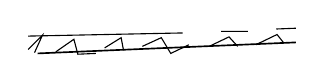
\begin{tikzpicture}[x=1cm,y=1cm]
\draw (0,.24) -- (1.96,.28) (2.45,.30) -- (2.79,.30)
      (3.15,.33) -- (3.40,.34);
\draw[semithick] (.12,.02) -- (3.40,.16);
\draw (0,.07)--(.18,.25)--(.08,.03)
  (.35,.04)--(.58,.20)--(.63,.01)--(.86,.02)
  (.97,.09)--(1.18,.22)--(1.21,.06)
  (1.45,.11)--(1.69,.22)--(1.81,.02)--(2.04,.13)
  (2.32,.12)--(2.55,.23)--(2.66,.11)
  (2.89,.13)--(3.16,.26)--(3.24,.16);
\end{tikzpicture}}\endgroup\par
Под датой видны наложенные горизонтальные и угловатые штрихи. Отдельные буквы не читаются.}
\end{GelfandAdjacentEvidence}
\begin{GelfandAdjacentEvidence}{GELFAND-P000834}{2}


\uuline{Лебедев (Митя)}

\uwave{О результатах Ритта и Кириллова по дифференциальной алгебре}.

\(M\) — гладкое многообразие, \(\dim M=n\)

\SourceFigure{GELFAND-P000834}{vector-bundle-arrow}{%
\begingroup\color{black}\GelfandFitDiagram{\begin{tikzpicture}[x=1cm,y=1cm,every node/.style={font=\small}]
\node (e) at (0,.63) {\(E\)};
\node (m) at (0,-.66) {\(M\)};
\draw[->] (e)--(m);
\node[anchor=west] at (.65,.18) {векторное};
\node[anchor=west] at (.65,-.14) {расслоение;};
\node at (.39,-.12) {—};
\end{tikzpicture}}\endgroup}
\end{GelfandAdjacentEvidence}
\begin{GelfandAdjacentEvidence}{GELFAND-P000834}{3}


\(\Gamma^\infty(E)\) — гладкие сечения.
\[
s_1,s_2\in\Gamma^\infty(E)
\]
Введем билинейную операцию: \([\cdot,\cdot]\):
\[
[s_1,s_2]\in\Gamma^\infty(E)
\]
\Unclear{GELFAND-P000834}{bracket-result-membership}{Знак перед \(\Gamma^\infty(E)\) наведён и предварительно прочитан как \(\in\).}
\end{GelfandAdjacentEvidence}
\begin{GelfandAdjacentEvidence}{GELFAND-P000834}{4}


а) билин., кососимм., тожд. Якоби

б) непр. в топ. равн. схд. произв. на компактах

\Unclear{GELFAND-P000834}{continuity-abbreviation}{Сокращение предварительно набрано «схд.». Между «х» и наведённым «д» возможна отдельная «о».}
\end{GelfandAdjacentEvidence}
\begin{GelfandAdjacentEvidence}{GELFAND-P000834}{5}


в) \(\operatorname{supp}[s_1,s_2]\subset
\operatorname{supp}s_1\cap\operatorname{supp}s_2\)
\qquad (локальность)

[зачёркнуто: \sout{…}] Это наз. \uwave{дифференциальной алгеброй Ли}.
\Incomplete{GELFAND-P000834}{cancelled-final-word}{В начале зачёркнутого фрагмента видна петля, похожая на «В». Остальные буквы не читаются.}
\end{GelfandAdjacentEvidence}



\Needspace{7\baselineskip}
\begin{GelfandAdjacentEvidence}{GELFAND-P000835}{1}
\SourcePage{GELFAND-P000835}{20}
\uwave{То же определение в лок. координатах}

Пусть \(F\) — слой; \(\dim F=1\)

\(x_1,\ldots,x_n\) — коорд. на базе.

Тогда локально
\begin{equation*}
[f,g]=\sum c_{k\ell}(x)\partial^k f\cdot\partial^\ell g,
\qquad k,\ell\text{ — мультииндексы}
\tag{1}
\end{equation*}
\uwave{Осн. рез. Кириллова}: классификация таких алгебр.

\uline{Теорема 1}. Все лок. алгебры со слоем разм. 1 исчерп. 2-мя (по существу)

\begin{equation*}
\text{а)}\quad M=\mathbb R^{2n},\qquad
[f,g]=\sum\left(\frac{\partial f}{\partial x_i}\frac{\partial g}{\partial y_i}
-\frac{\partial f}{\partial y_i}\frac{\partial g}{\partial x_i}\right)
\tag{2}
\end{equation*}
\Unclear{GELFAND-P000835}{poisson-overwriting}{В первом числителе для \(g\) и во втором знаменателе с \(y_i\) видны наложенные штрихи. Ранние начертания не различаются.}
\end{GelfandAdjacentEvidence}
\begin{GelfandAdjacentEvidence}{GELFAND-P000835}{2}


\begin{equation*}
\begin{gathered}
\text{б)}\quad M=\mathbb R^{2n+1},\quad
X_i=\frac{\partial}{\partial x_i},\quad
Y_i=\frac{\partial}{\partial y_i}+x_i\frac{\partial}{\partial z},\quad
Z=\frac{\partial}{\partial z}\text{ — вект. поля}
\end{gathered}
\tag{3}
\end{equation*}
\Unclear{GELFAND-P000835}{contact-vector-sign}{В записи \(Y_i\) перед \(x_i\partial/\partial z\) виден плюс.}
\end{GelfandAdjacentEvidence}
\begin{GelfandAdjacentEvidence}{GELFAND-P000835}{3}

\begin{equation*}
[f,g]=fZg-gZf+\sum_{i=1}^{n}(X_i f\cdot Y_i g-X_i g\cdot Y_i f)
\tag*{$(3)_1$}
\end{equation*}
\Unclear{GELFAND-P000835}{contact-bracket-sign}{Перед суммой в \((3)_1\) виден плюс.}
\end{GelfandAdjacentEvidence}
\begin{GelfandAdjacentEvidence}{GELFAND-P000835}{4}

Все остальные им формально изоморфны.

\uline{Ритт}.

\uwave{Дифференциальная группа Ли и дифф. алгебра Ли}.

\SourceFigure{GELFAND-P000835}{dimension-diagram}{%
\begingroup\color{black}\GelfandFitDiagram{\begin{tikzpicture}[x=.83cm,y=.83cm,every node/.style={font=\scriptsize,inner sep=1.5pt}]
\draw[->] (0,0)--(4.88,0) node[above right] {\(\dim M\)};
\draw[->] (0,0)--(0,-3.9) node[left] {\(\dim F\)};
\draw (.68,.01)--(.68,-.22);
\node[above] at (.68,.03) {1};
\node[left] at (0,-.68) {1};
\node[left] at (0,-1.4) {2};
\draw (0,-.68)--(4.88,-.68) node[right] {Кириллов};
\fill (0,-.68) circle[radius=.065cm];
\draw[dashed] (0,-1.4)--(4.03,-1.4);
\draw[dashed] (.68,-.82)--(.68,-1.14);
\draw (.68,-1.4) circle[radius=.22cm];
\fill (.68,-1.4) circle[radius=.09cm];
\node[below] at (4.19,-1.31) {?};
\draw[->] (1.14,-2.36) to[bend right=14] (.88,-1.62);
\draw[->] (4.86,-2.36) to[bend right=16] (4.42,-1.64);
\node[align=center,below] at (2.0,-2.37) {10 алгебр\\Ритта};
\node[align=left,below] at (5.18,-2.37) {здесь\\лишь\\\relax [правдопод.]\\\relax [версия]};
\end{tikzpicture}}\endgroup\par
На правом поле. Последние две строки подписи справа предположительно читаются «правдопод. / версия».}
\end{GelfandAdjacentEvidence}
\begin{GelfandAdjacentEvidence}{GELFAND-P000835}{5}


Рассмотрим ряды
\begin{equation*}
\sigma_1=\sum_{i\ge 1}a_i\,a\,\xi^{-(i+1)}
\tag{4}
\end{equation*}
\Unclear{GELFAND-P000835}{series-extra-mark}{Между \(a_i\) и \(\xi\) стоит отдельный тёмный знак, похожий на \(a\).}
\end{GelfandAdjacentEvidence}
\begin{GelfandAdjacentEvidence}{GELFAND-P000835}{6}


[зачёркнуто: \sout{…}] и коммутатор
\Incomplete{GELFAND-P000835}{cancelled-before-commutator}{Небольшая запись слева перечёркнута. Исходные знаки не читаются.}
\end{GelfandAdjacentEvidence}
\begin{GelfandAdjacentEvidence}{GELFAND-P000835}{7}

\begin{equation*}
[\sigma_1,\sigma_2]=\sigma_1\cdot\sigma_2-\sigma_2\cdot\sigma_1
\tag{5}
\end{equation*}
(здесь \(\dim M=1\), \(\dim F=\infty\)).

\([\xi,x]=1\) — этим всё определяется.

\SourceFigure{GELFAND-P000835}{double-divider}{%
\begingroup\color{black}\GelfandFitDiagram{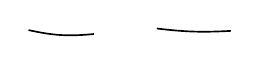
\begin{tikzpicture}
\draw[semithick] (0,0) to[bend right=9] (.83,-.05);
\draw[semithick] (1.63,.02) to[bend right=5] (2.57,-.01);
\end{tikzpicture}}\endgroup}
\end{GelfandAdjacentEvidence}
\begin{GelfandAdjacentEvidence}{GELFAND-P000835}{8}


\(\mathcal F\) — дифф. поле хар-ки \(0\), \qquad «\(\partial=\frac{\partial}{\partial x}\)»

\(y_1(x),\ldots,y_n(x)\) — дифф. независимые

Рассм. кольцо
\begin{equation*}
\mathcal F[[y_i^{(j)}]]\simeq\bigoplus\mathcal F_\tau,
\qquad \tau\text{ — «порядок» — степень — кол-во сомнож.}
\tag{6}
\end{equation*}
\Unclear{GELFAND-P000835}{ring-grading}{У знака отношения волнистая верхняя черта. Условно набрано \(\simeq\). Индекс предварительно прочитан как \(\tau\).}
\end{GelfandAdjacentEvidence}
\begin{GelfandAdjacentEvidence}{GELFAND-P000835}{9}


\uwave{Форм. дифф. группа Ли} \(\equiv\) форм. групп. закон \(\equiv\) набор ф-й
\begin{equation*}
U_i\in\mathcal F[[u_i^{(j)},v_\ell^{(m)}]]
\tag{7}
\end{equation*}
\Unclear{GELFAND-P000835}{differential-variables}{У \(v\) справа вверху виден короткий горизонтальный штрих, соединённый с буквой. Возможно, это отдельная черта.}
\end{GelfandAdjacentEvidence}


Удовл. 2-м аксиомам:

а) \(U_i(\bar u,0)=\bar u_i,\qquad U_i(0,\bar v)=\bar v_i\)

б) ассоциат.


\Needspace{7\baselineskip}
\begin{GelfandAdjacentEvidence}{GELFAND-P000836}{1}
\SourcePage{GELFAND-P000836}{unlabelled}
\uline{Пример}.

\SourceFigure{GELFAND-P000836}{taylor-vertical-relation}{%
\begingroup\color{black}\GelfandFitDiagram{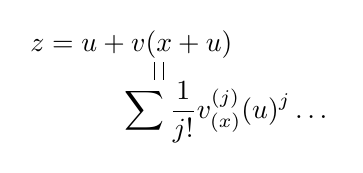
\begin{tikzpicture}[x=1cm,y=1cm,every node/.style={inner sep=1pt}]
\node[anchor=west] at (0,0) {\(z=u+v(x+u)\)};
\draw (1.62,-.23)--(1.62,-.45) (1.73,-.23)--(1.73,-.45);
\node[anchor=west] at (1.20,-.86)
  {\(\displaystyle\sum\frac{1}{j!}v^{(j)}_{(x)}(u)^j\,\text{\sout{…}}\)};
\end{tikzpicture}}\endgroup\par
Под \(v(x+u)\) две вертикальные черты между формулой и рядом.}
\end{GelfandAdjacentEvidence}
\begin{GelfandAdjacentEvidence}{GELFAND-P000836}{2}

\Unclear{GELFAND-P000836}{expansion-cancel}{После \((u)^j\) зачёркнута ещё одна запись. Возможно, это \(u^j\).}
\end{GelfandAdjacentEvidence}
\begin{GelfandAdjacentEvidence}{GELFAND-P000836}{3}


(для группы диффеоморфизмов, ост. \(\downarrow x\) на место)
\Unclear{GELFAND-P000836}{diffeomorphism-mark}{Между «ост.» и \(x\) короткий вертикальный штрих, условно переданный стрелкой вниз.}
\end{GelfandAdjacentEvidence}
\begin{GelfandAdjacentEvidence}{GELFAND-P000836}{4}


Форм. ряд:
\[
\begin{aligned}
U&=\sum_{k=0}^{\infty}P_k,\\
P_k&=\text{однор. многоч. степ. }k\text{ от }
u_1,\ldots,u_n,u_1^{(1)},\ldots,u_n^{(1)},
\end{aligned}
\]
над дифф. полем (поле функций с дифф.)
\Unclear{GELFAND-P000836}{formal-overwrite}{Начало слова «функций» переписано поверх прежних штрихов. Исходное начертание не читается.}
\end{GelfandAdjacentEvidence}
\begin{GelfandAdjacentEvidence}{GELFAND-P000836}{5}


\uline{Теорема} 2

\uwave{Классификац. дифф. групп со слоем разм.} 2

\(A^h.\)
\SourceFigure{GELFAND-P000836}{group-operation-callout}{%
\begingroup\color{black}\GelfandFitDiagram{\begin{tikzpicture}[x=1cm,y=1cm,every node/.style={inner sep=1pt}]
\node at (0,0) {\(u(x)\,dx^{-h}+v(x)\,dx^{-h}\)};
\draw[->] (-.17,-.66)--(-.10,-.27);
\node[align=center,below,font=\small] at (-.13,-.70)
  {операция\\в группе};
\end{tikzpicture}}\endgroup}
\end{GelfandAdjacentEvidence}

\[
u\circ v=u+v
\]
\[
\Pi:\qquad u\circ v=u+v(x+u)
\]
Все группы — расш. \(\Pi\) с помощью \(A^h\).


\Needspace{7\baselineskip}
\begin{GelfandAdjacentEvidence}{GELFAND-P000837}{1}
\SourcePage{GELFAND-P000837}{unlabelled}
\uline{2/IV–78 г.}\qquad \uline{Сем. Гельфанда}
\Unclear{GELFAND-P000837}{date-year}{Последняя цифра года предварительно прочитана как 8. Возможно 9.}
\end{GelfandAdjacentEvidence}
\begin{GelfandAdjacentEvidence}{GELFAND-P000837}{2}


\uline{К. Шабат}. \quad Из раб. \uwave{Гриффитса и Чжэня}.
\Unclear{GELFAND-P000837}{speaker-initial}{Инициал предварительно прочитан как «К.». Возможно «Ю.».}
\end{GelfandAdjacentEvidence}
\begin{GelfandAdjacentEvidence}{GELFAND-P000837}{3}


Ткань — конечное число слоений с трансверс. слоями. Она строится \uline{на} многообразии.

(сеть) — \uline{Web}

\[
X\subset P^n,\qquad \dim X=m,\qquad \operatorname{deg}X=d.
\]
[Под \(X\):] проект. мн-зие (алгебр.)

Ткань в \(\mathrm{Gr}(m,n-m)\), точнее в нек. его открытом мн-ве:
\Unclear{GELFAND-P000837}{grassmann-qualifier}{Между «в» и «открытом» предварительно прочитано «нек. его». Середина записи бледная.}
\end{GelfandAdjacentEvidence}
\begin{GelfandAdjacentEvidence}{GELFAND-P000837}{4}


\begin{equation*}
U=\{H\mid H\cdot X=d\text{ разных точек}\}
\quad\text{— открытое мн-во}
\tag{1}
\end{equation*}

\SourceFigure{GELFAND-P000837}{curve-line-intersections}{%
\begingroup\color{black}\GelfandFitDiagram{\begin{tikzpicture}[x=1cm,y=1cm,line width=.65pt]
\draw (-.35,-1.15)--(.43,1.35);
\draw (.88,.66) .. controls (.68,.82) and (.46,.90) .. (.29,.83)
 .. controls (-.23,.72) and (-.48,.29) .. (-.01,.18)
 .. controls (.45,.23) and (.84,.09) .. (.78,-.28)
 .. controls (.73,-.68) and (.28,-.61) .. (-.20,-.66)
 .. controls (-.45,-.69) and (-.61,-.63) .. (-.79,-.63);
\draw[line width=1.35pt] (-.78,-.63)--(-.20,-.66);
\fill (.29,.83) circle[radius=.072cm];
\fill (.065,.18) circle[radius=.072cm];
\fill (-.20,-.66) circle[radius=.086cm];
\end{tikzpicture}}\endgroup}
\end{GelfandAdjacentEvidence}
\begin{GelfandAdjacentEvidence}{GELFAND-P000837}{5}


([зачёркнуто: \sout{…}] когда есть кратность — выбрасываем)
\Incomplete{GELFAND-P000837}{multiplicity-cancel}{Первое слово в скобках зачёркнуто. Исходные буквы неразличимы.}
\end{GelfandAdjacentEvidence}
\begin{GelfandAdjacentEvidence}{GELFAND-P000837}{6}


\uline{И.М.Г.}

\uwave{Ф-ла Крофтона}: длина кривой = среднее число точек, по к-рым её пересекает прямая
(среднее по прямым отн. инвар. меры).

Гриффитс и Чжэнь, вдохновл. раб. Пенроуза, обобщили это на многомерный [вписано слева снизу: \(\leftarrow\) случай].
\Unclear{GELFAND-P000837}{multidimensional-insertion}{Слово «случай» стоит слева под строкой. Над ним короткая стрелка влево.}
\end{GelfandAdjacentEvidence}
\begin{GelfandAdjacentEvidence}{GELFAND-P000837}{7}


\uwave{Слой, прох. через точку} \(H_0\in U\), \uwave{состоит из}
[зачёркнуто: \sout{поверхностей}].
\Unclear{GELFAND-P000837}{slice-cancel-right}{Зачёркнутое слово предварительно прочитано «поверхностей».}
\end{GelfandAdjacentEvidence}
\begin{GelfandAdjacentEvidence}{GELFAND-P000837}{8}


[зачёркнуто: \sout{точек \(X\)}] \uwave{плоскостей}
\[
\{H\in U\mid \exists i\in\{1,2,\ldots,d\};\ \underline{P}_i\in H\}.
\]
\Unclear{GELFAND-P000837}{slice-cancel-left}{В начале строки зачёркнуты «точек \(X\)». У первого \(P_i\) видна короткая черта снизу.}
\end{GelfandAdjacentEvidence}
\begin{GelfandAdjacentEvidence}{GELFAND-P000837}{9}

\[
H_0\cdot X=P_1+\ldots+P_d
\]
\begin{equation*}
\{H\in U\mid \exists i\in\{1,2,\ldots,d\},\ P_i\in H\}
\tag{2}
\end{equation*}

Это слоение коразмерности 1. (так зд. плоскости разд. на листы, сами могут пересечься)
\Unclear{GELFAND-P000837}{foliation-note}{Сокращения предварительно прочитаны «зд.» и «разд.».}
\end{GelfandAdjacentEvidence}
\begin{GelfandAdjacentEvidence}{GELFAND-P000837}{10}


\uline{И.М.Г.}\quad [зачёркнуто: \sout{Вопросы}]
\Unclear{GELFAND-P000837}{problem-cancel}{Зачёркнутое слово предварительно читается «Вопросы».}
\end{GelfandAdjacentEvidence}
\begin{GelfandAdjacentEvidence}{GELFAND-P000837}{11}


\uline{Задача}: \uwave{есть 3 слоения} (трансверс.) Когда их можно выпрямить?
[Под «есть 3 слоения» вписано:] \uwave{на плоск.}.

(2 всегда!!)

3 можно выпр. \(\Leftrightarrow\) она гексагональна, т. е.

\(\approx1927\) г.

\SourceFigure{GELFAND-P000837}{hexagonal-path}{%
\begingroup\color{black}\GelfandFitDiagram{\begin{tikzpicture}[x=1cm,y=1cm,line width=.62pt]
\draw (-1.45,.07)--(-1.16,.12)--(-.95,.05)--(-.39,.08)--(0,0)
      --(.70,-.08)--(1.34,-.17);
\draw (-.61,1.22)--(-.26,.57)--(0,0)--(.38,-.56)--(.55,-.88);
\draw[->] (.98,.97)--(.51,.55)--(0,0)--(-.53,-.52)--(-1.18,-1.22);
\draw[line width=.8pt] (-.95,.05)--(-.26,.57)--(.51,.55);
\draw[line width=.8pt] (-.95,.05)--(-.53,-.52)--(.38,-.56)--(.70,-.08);
\fill (-1.45,.07) circle[radius=.046cm];
\fill (-.26,.57) circle[radius=.060cm];
\draw (.51,.55) circle[radius=.09cm];
\draw (-.95,.05) circle[radius=.068cm];
\draw (-.53,-.52) circle[radius=.065cm];
\fill (.38,-.56) circle[radius=.052cm];
\fill (0,0) circle[radius=.075cm];
\fill (.70,.037)--(.83,-.08)--(.70,-.21)--(.61,-.08)--cycle;
\fill (-.32,1.05) circle[radius=.032cm];
\end{tikzpicture}}\endgroup\par
Три направления, малые кружки и утолщённые узлы воспроизведены по видимым штрихам. Порядок обхода и направления некоторых малых стрелок неразличимы.}
\end{GelfandAdjacentEvidence}
\begin{GelfandAdjacentEvidence}{GELFAND-P000837}{12}


— такой путь (инфинитезимальный) должен быть замкнут. — что-то вроде кривизны.

\SourceFigure{GELFAND-P000837}{separate-footer-strokes}{%
\begingroup\color{black}\GelfandFitDiagram{\begin{tikzpicture}
\fill (0,0) circle[radius=.038cm];
\draw (0,0) to[bend right=5] (.45,-.02) -- (1.35,0);
\draw (2.05,.04) -- (3.35,.16);
\end{tikzpicture}}\endgroup}
\end{GelfandAdjacentEvidence}



\Needspace{7\baselineskip}
\begin{GelfandAdjacentEvidence}{GELFAND-P000838}{1}
\SourcePage{GELFAND-P000838}{29}
Теперь \(m=1\).
\[
\begin{array}{@{}l@{}}
X\subset P^n\\[-.15em]
\vert\\[-.15em]
\text{проект. \uwave{кривая}}
\end{array}
\]

\(\check P^n\) — двойств. проект. пр-во.
\begin{equation*}
\check{\mathbb P}^{\,n}\supset U
=\{H\mid H\circ X=d\text{ разных точек}\}
\tag{3}
\end{equation*}
\Unclear{GELFAND-P000838}{intersection-sign}{Между \(H\) и \(X\) виден малый овал. Условно набрано \(\circ\).}
\end{GelfandAdjacentEvidence}
\begin{GelfandAdjacentEvidence}{GELFAND-P000838}{2}


На \(U\) получ. ткань коразмерности 1.

\SourceFigure{GELFAND-P000838}{pencil-diagram}{%
\begingroup\color{black}\GelfandFitDiagram{\begin{tikzpicture}[x=.019cm,y=-.019cm,line cap=round,line width=.5pt]
\coordinate (a) at (154,56);
\coordinate (b) at (123,112);
\coordinate (c) at (98,177);
\draw[line width=.85pt] (197,77) .. controls (177,55) and (168,53) .. (a)
 .. controls (101,49) and (59,103) .. (b)
 .. controls (160,111) and (176,130) .. (172,150)
 .. controls (164,168) and (140,173) .. (c) -- (47,174);
\draw (112,33)--(a)--(193,83) (138,23) .. controls (145,27) and (151,46) .. (a)
 -- (170,101) (167,30)--(a)--(b)--(c)--(90,201);
\draw (205,26)--(a)--(119,77) (213,37)--(a)--(105,76);
\draw (105,92)--(b) .. controls (131,120) and (137,127) .. (140,141);
\draw (121,90)--(b)--(122,147) (77,123)--(b)--(165,103)
 (88,134)--(b)--(147,96);
\draw (51,196)--(c)--(135,159) (48,213)--(c)--(129,152)
 (90,147)--(c)--(104,216) (73,157) .. controls (84,151) and (93,171) .. (c)
 -- (113,201);
\fill (a) circle[radius=.066cm];
\fill (b) circle[radius=.066cm];
\fill (c) circle[radius=.071cm];
\end{tikzpicture}}\endgroup\par
Три центра и различимые штрихи воспроизведены. Часть штрихов сливается друг с другом, поэтому их точное число не установлено.}
\end{GelfandAdjacentEvidence}
\begin{GelfandAdjacentEvidence}{GELFAND-P000838}{3}


\uwave{Абелево ур-е для ткани}.

\SourceFigure{GELFAND-P000838}{grid-geometry}{%
\begingroup\color{black}\GelfandFitDiagram{\begin{tikzpicture}[x=.016cm,y=-.016cm,line width=.55pt]
\draw (120,72) .. controls (128,33) and (165,18) .. (191,20)
 .. controls (218,22) and (233,50) .. (230,72)
 .. controls (227,101) and (205,130) .. (170,136)
 .. controls (132,145) and (109,121) .. (120,72);
\draw (152,57) .. controls (180,52) and (178,93) .. (179,128);
\draw (190,47) .. controls (204,58) and (205,96) .. (203,116);
\draw (217,45) .. controls (228,38) and (230,86) .. (234,106);
\draw (140,97) .. controls (164,73) and (211,56) .. (252,38);
\draw (150,108) .. controls (192,91) and (219,78) .. (246,67);
\draw (156,129) .. controls (178,116) and (203,111) .. (229,102);
\node[anchor=west,font=\small] at (19,42) {\([u]\)};
\end{tikzpicture}}\endgroup}
\end{GelfandAdjacentEvidence}
\begin{GelfandAdjacentEvidence}{GELFAND-P000838}{4}

\Unclear{GELFAND-P000838}{grid-label}{Слева от овала знак условно передан как \(u\). Возможно \(U\).}
\end{GelfandAdjacentEvidence}
\begin{GelfandAdjacentEvidence}{GELFAND-P000838}{5}


\begin{equation*}
\begin{cases}
u_1=\mathrm{const}.\\
\vdots\\
u_n=\mathrm{const}
\end{cases}
\tag{4}
\end{equation*}

\uwave{Аб. ур-е для ткани имеет вид}:
\begin{equation*}
\sum_{i=1}^{d}f_i(u_i)\,du_i=0,\qquad
\sum_{i=1}^{d}f_i(u_i)\,du_i\in\Omega^1(U)
\tag{5}
\end{equation*}

Между нормальными векторами — зависимость (кокас. векторы), причём коэффициенты имеют вид \(f_i(u_i)\).

\uline{Ранг ткани} \(\underset{\mathrm{def}}{=}\)
\uwave{макс. число лин. независимых абелевых ур-й}, \uwave{к-рым она удовлетворяет}.

\uuline{Утв. 1}
\uwave{Ранг ткани, построенной по кривой рода} \(g\), \uwave{равен} \(g\).

[зачёркнуто: \sout{Еще теорема 1 — При условиях}
\sout{\(n\ge3,\ d\ge2n\)}]
\Unclear{GELFAND-P000838}{cancelled-heading}{Первое зачёркнутое слово предварительно прочитано «Еще».}
\end{GelfandAdjacentEvidence}
\begin{GelfandAdjacentEvidence}{GELFAND-P000838}{6}

\Unclear{GELFAND-P000838}{cancelled-hypotheses}{Под зачёркиванием предварительно прочитано \(n\ge3,\ d\ge2n\).}
\end{GelfandAdjacentEvidence}
\begin{GelfandAdjacentEvidence}{GELFAND-P000838}{7}


\uline{Теорема} 1 (Chern, 193 ?)
\Unclear{GELFAND-P000838}{chern-year}{В рукописи после 193 стоит знак вопроса.}
\end{GelfandAdjacentEvidence}
\begin{GelfandAdjacentEvidence}{GELFAND-P000838}{8}


\SourceFigure{GELFAND-P000838}{rank-callouts}{%
\begingroup\color{black}\GelfandFitDiagram{\begin{tikzpicture}[x=1cm,y=1cm,every node/.style={font=\small}]
\node[anchor=west] at (0,0) {\uwave{Ранг \(d\)-ткани}};
\node[anchor=west] at (3.65,0) {\(\le\pi(n,d)\)};
\draw[->] (.10,-1.32)--(.61,-.29);
\node[anchor=west,align=left] at (0,-1.53) {(произв. ткань!)};
\node[anchor=west,align=left] at (1.25,-.90) {(\uwave{в \(n\)-мерном}\\\uwave{мн-зии})};
\node[anchor=west,align=left] at (3.65,-.40) {(число Кастельнуово)};
\end{tikzpicture}}\endgroup}
\end{GelfandAdjacentEvidence}


\begin{equation*}
\pi(n,d)\underset{\mathrm{def}}{=}
\text{макс. род кривой степени }d\text{ в }\mathbb P^n,
\qquad \underline{\underline{n,d\ge2}}.
\tag{6}
\end{equation*}

Есть короткая ф-ла
\begin{equation*}
\pi(n,d)=m\left(d-\frac12(m+1)(n-1)-1\right),
\quad\text{где }m=\left[\frac{d-1}{n-1}\right].
\tag{7}
\end{equation*}


\Needspace{7\baselineskip}
\begin{GelfandAdjacentEvidence}{GELFAND-P000839}{1}
\SourcePage{GELFAND-P000839}{unlabelled}
\uuline{Теорема 2.}

(основная)

\uwave{Если} \(n\ge3,\ d\ge2n\) и \uwave{\(d\)-ткань имеет ранг} \(\pi(n,d)\),

\uwave{то}

1) \uwave{Она линеаризуема}

2) \uwave{Она продолжается до ткани, получ. из} \(X\subset\mathbb P^n\).

Объясняется связь таких ур-й и абелевых дифференциалов.

\uline{Ссылка:}

\uwave{(Sonderdruck aus) Jber. d. Dt. Math.-Verein}, \(80\) (\(1978\)), 13–110

[Под «Sonderdruck aus»: \uwave{оттиск} из.]

(Jahresberichte der Deutsche[…] Math. Vereinigung)
\Unclear{GELFAND-P000839}{reference-expansion}{Окончание после «Deutsche» неуверенно. Возможны «Deutschen» и «Deutscher».}
\end{GelfandAdjacentEvidence}
\begin{GelfandAdjacentEvidence}{GELFAND-P000839}{2}


[зачёркнуто: \sout{…}]
\Incomplete{GELFAND-P000839}{reference-cancelled-word}{Под ссылкой зачёркнуто слово. Начальная петля различима, остальные буквы скрыты штрихами.}
\end{GelfandAdjacentEvidence}
\begin{GelfandAdjacentEvidence}{GELFAND-P000839}{3}


Развивается геометрия
\SourceFigure{GELFAND-P000839}{projective-connection-underlining}{%
\begingroup\color{black}\GelfandFitDiagram{\begin{tikzpicture}[x=1cm,y=1cm,every node/.style={inner sep=1pt}]
\node[anchor=west] at (0,0) {проективных связностей.};
\draw[->] (.93,-.28)--(0,-.28);
\draw (1.70,-.28)--(3.89,-.28);
\end{tikzpicture}}\endgroup\par
Слева штрих со стрелкой влево, справа отдельная черта под словами.}
\end{GelfandAdjacentEvidence}
\begin{GelfandAdjacentEvidence}{GELFAND-P000839}{4}


\uline{Замолодчиков А.} (Саша) \quad Пусть есть \(S_{ij}^{k\ell}(\lambda)\)
\Unclear{GELFAND-P000839}{initial-matrix-indices}{Верхние индексы предварительно прочитаны \(k,\ell\). Они соприкасаются с чертой от предыдущей строки.}
\end{GelfandAdjacentEvidence}
\begin{GelfandAdjacentEvidence}{GELFAND-P000839}{5}


Пусть ещё есть картина:

\(L\) прямых, углы \(\lambda_1,\ldots,\lambda_L\)

\(\lambda_i\) в порядке возрастания

(от какой-то прямой

[зачёркнуто: \sout{То}]
\Unclear{GELFAND-P000839}{cancelled-to}{Зачёркнутое слово предварительно прочитано «То».}
\end{GelfandAdjacentEvidence}
\begin{GelfandAdjacentEvidence}{GELFAND-P000839}{6}


\SourceFigure{GELFAND-P000839}{single-vertex-diagram}{%
\begingroup\color{black}\GelfandFitDiagram{\begin{tikzpicture}[x=1cm,y=1cm,line width=.72pt]
\draw (-.72,.85)--(.04,0)--(.75,-.77);
\draw (.95,.79)--(.04,0)--(-.70,-.65);
\draw[->,thick] (.39,-.38)--(.60,-.62);
\draw[->,thick] (-.23,-.24)--(-.61,-.58);
\draw (.04,0) circle[radius=.083cm];
\node at (-.58,1.04) {\([c]\)};
\node at (1.20,.75) {\(j\)};
\node at (-.62,-.95) {\(i\)};
\node at (1.25,-.42) {\(k\)};
\end{tikzpicture}}\endgroup\par
Верхний левый знак по очертанию похож на \(c\), возможно \(\ell\).}
\end{GelfandAdjacentEvidence}
\begin{GelfandAdjacentEvidence}{GELFAND-P000839}{7}


индексы \(=1,2,\ldots,N\)

\SourceFigure{GELFAND-P000839}{many-lines-diagram}{%
\begingroup\color{black}\GelfandFitDiagram{\begin{tikzpicture}[x=.013cm,y=-.013cm,line width=.65pt]
\draw (12,181) .. controls (86,175) and (121,172) .. (168,174)
 .. controls (222,175) and (270,182) .. (325,176);
\draw (40,256) .. controls (60,218) and (68,211) .. (86,178)
 -- (133,116)--(166,81)--(237,14);
\draw (76,12)--(100,51)--(133,116)--(166,172)
 .. controls (177,200) and (185,224) .. (193,251);
\draw (31,21) .. controls (46,21) and (78,40) .. (100,51)
 -- (166,81) .. controls (208,105) and (249,151) .. (280,179)
 -- (360,241);
\draw (228,22)--(238,15)--(234,25)
 (47,247)--(40,256)--(49,251)
 (355,233)--(360,241)--(352,237);
\foreach \x/\y/\r in {100/51/7,166/81/6,133/116/6,86/178/7,166/172/7,280/179/9}
  \draw (\x,\y) circle[radius=\r];
\end{tikzpicture}}\endgroup\par
Шесть обведённых пересечений. Короткие штрихи на концах воспроизведены по очертаниям. Направления некоторых стрелок неясны.}
\end{GelfandAdjacentEvidence}
\begin{GelfandAdjacentEvidence}{GELFAND-P000839}{8}


Узлу — матрица; Хвостам — индексы, по связям — суммирую.

Получ. матрица (большая). Интересно её повед. при \(L\to\infty\)?
\[
Z^{j_1\ldots j_L}_{i_1\ldots i_L}(\lambda_1,\ldots,\lambda_L).
\]

\uline{Проблема 1.} Есть асимптотика

(как сосч. точно — неизвестно)
\Unclear{GELFAND-P000839}{problem-parenthesis}{Слова предварительно прочитаны «сосч. точно». Возможно «сосч. её».}
\end{GelfandAdjacentEvidence}
\begin{GelfandAdjacentEvidence}{GELFAND-P000839}{9}

\begin{equation*}
\ln Z\text{\sout{…}}\sim\text{пропорц. числу узлов}
\tag{1}
\end{equation*}
\Unclear{GELFAND-P000839}{hatched-indices}{После \(Z\) заштрихованы знаки, похожие на индексы \(j_1\ldots j_L,\ i_1\ldots i_L\) и аргументы \((\lambda_1,\ldots,\lambda_L)\). Под штриховкой не все знаки различимы.}
\end{GelfandAdjacentEvidence}
\begin{GelfandAdjacentEvidence}{GELFAND-P000839}{10}


\begin{equation*}
Z\underset{\mathrm{df}}{=}Z^{i_1\ldots i_L}_{i_1\ldots i_L}
\qquad\text{(«след»)}\qquad\text{(суммир. по повт.)}
\tag{2}
\end{equation*}
Каждой прямой \(\leadsto\) параметр \(\lambda_j\)

(нумеруются лучи по часовой стрелке \uwave{\(i_1,\ldots,i_L,j_1,\ldots,j_L\)}.)
\Unclear{GELFAND-P000839}{clockwise-indices}{Первые нижние индексы при \(i\) и \(j\) предварительно переданы цифрой \(1\). Начертание похоже также на \(L\).}
\end{GelfandAdjacentEvidence}
\begin{GelfandAdjacentEvidence}{GELFAND-P000839}{11}


\begin{equation*}
Z^{j_1\ldots j_L}_{i_1\ldots i_L}
=\sum_{\substack{\text{внутр.}\\\text{\sout{…}}\\\text{отрезкам}}}
\left(\prod_{\substack{\text{точкам}\\\text{пересеч.}}}
S^{**}_{**}(\lambda_a-\lambda_b)\right)
\tag{3}
\end{equation*}
\Incomplete{GELFAND-P000839}{sum-cancelled-word}{Средняя строка под суммой зачёркнута. Слово не читается.}
\end{GelfandAdjacentEvidence}
\begin{GelfandAdjacentEvidence}{GELFAND-P000839}{12}


[Справа под формулой:] естеств. упорядочение из напр. прямых
\Unclear{GELFAND-P000839}{ordering-overwritten-ending}{Конец слова «прямых» переправлен. Первоначальные штрихи неразличимы.}
\end{GelfandAdjacentEvidence}


есть горизонт. прямая, к-рую они пересек. в самом низу.

Есть ф-и, к-рые не мен. при паралл. переносе.


\Needspace{7\baselineskip}
\begin{GelfandAdjacentEvidence}{GELFAND-P000840}{1}
\SourcePage{GELFAND-P000840}{30}
\SourceFigure{GELFAND-P000840}{indexed-lines}{%
\begingroup\color{black}\GelfandFitDiagram{\begin{tikzpicture}[x=.01cm,y=-.01cm,line width=.65pt]
\draw (270,185)--(408,416) (388,110)--(349,441) (202,331)--(464,124);
\fill (305,249) circle[radius=.55mm];
\fill (378,192) circle[radius=.55mm];
\fill (361,338) circle[radius=.55mm];
\node[left] at (258,169) {\(i_1\)};
\node[above left] at (384,108) {\(i_2\)};
\node[above right] at (470,125) {\(i_L\)};
\node[below left] at (201,347) {\(j_L\)};
\node[below] at (346,450) {\(j_2\)};
\node[below right] at (410,423) {\(j_1\)};
\end{tikzpicture}}\endgroup}
\end{GelfandAdjacentEvidence}
\begin{GelfandAdjacentEvidence}{GELFAND-P000840}{2}


\uline{Ассоциат.}: \(Z\) не зав. от взаимного распол. прямых.

Достат., чтоб вып. для 3-х прямых:

\SourceFigure{GELFAND-P000840}{three-lines-equality}{%
\begingroup\color{black}\GelfandFitDiagram{\begin{tikzpicture}[x=.010cm,y=-.010cm,line width=.65pt,line cap=round]
\draw (24,177)--(165,68) (42,51)--(141,156) (73,32)--(61,165);
\draw[line width=1.4pt] (103,119) .. controls (119,132) and (130,136) .. (140,155);
\node at (258,99) {\(=\)};
\draw (348,95)--(466,182) (372,148)--(469,55) (439,65)--(425,188);
\end{tikzpicture}}\endgroup\par
Утолщение на нисходящей линии слева может быть повторной обводкой или стрелкой.}
\end{GelfandAdjacentEvidence}
\begin{GelfandAdjacentEvidence}{GELFAND-P000840}{3}


\uline{Утв. 2.} сущ. такие матрицы.

\uwave{Об асимптотике}:

\begin{equation*}
\ln Z^{j_1\ldots j_L}_{i_1\ldots i_L}\sim L^2
\qquad\text{при }L\to\infty\tag{4}
\end{equation*}

(\uwave{если без ассоциативности}) и асимпт. не зав. от выбора инд. \(i\) и \(j\).

[Под «асимпт.»: (гл. член.)]

\uuline{Утв.} 3. Асимптотика при \(L\to\infty\)

\begin{equation*}
\ln Z(\lambda_1,\ldots,\lambda_L)
=\sum_{a>b=1}^{L}f(\lambda_a-\lambda_b)+\text{остат. член}\tag{5}
\end{equation*}
\Unclear{GELFAND-P000840}{asymptotic-index-limit}{Нижний предел записан «\(a>b=1\)». Верхний предел \(L\).}
\end{GelfandAdjacentEvidence}
\begin{GelfandAdjacentEvidence}{GELFAND-P000840}{4}


(своб. эн. большой системы \(=\) сумма парных

\uline{Мнение}: есть \(L\) сортов частиц; они движ. по прямым и сталкиваются; при столкн. они сохр. скорости, но меняют \uuline{цвет}
\Unclear{GELFAND-P000840}{particle-model-heading}{Заголовок предварительно прочитан «Мнение».}
\end{GelfandAdjacentEvidence}
\begin{GelfandAdjacentEvidence}{GELFAND-P000840}{5}

\Unclear{GELFAND-P000840}{modified-velocity-word}{Начальные штрихи слова «скорости» переправлены. Предшествующее начертание неразличимо.}
\end{GelfandAdjacentEvidence}
\begin{GelfandAdjacentEvidence}{GELFAND-P000840}{6}


[Под «цвет»: (сорт)]

Здесь \(Z\) — \(S\)-матрица;

Есть интерпр., когда \(Z\) — стат. сумма

Веса \(S\) — \(\exp\) от потенциала. (вероятности?)

Есть нач. и \uwave{конечные расцветки} \(i_1,\ldots,i_L\)
\[
j_1,\ldots,j_L.
\]

\SourceFigure{GELFAND-P000840}{particle-divider}{%
\begingroup\color{black}\GelfandFitDiagram{\begin{tikzpicture}[x=1cm,y=1cm,line width=.45pt]
\draw (0,0) .. controls (1.1,.10) and (2.2,.12) .. (3.06,.07)
 .. controls (3.41,.06) and (3.56,.03) .. (3.73,-.04)
 .. controls (4.13,-.09) and (5.23,-.11) .. (6.05,-.075)
 .. controls (6.48,-.063) and (6.83,-.079) .. (7.16,-.095);
\end{tikzpicture}}\endgroup}
\end{GelfandAdjacentEvidence}
\begin{GelfandAdjacentEvidence}{GELFAND-P000840}{7}


\uuline{А. З.}

\SourceFigure{GELFAND-P000840}{spin-lines-diagram}{%
\begingroup\color{black}\GelfandFitDiagram{\begin{tikzpicture}[x=.011cm,y=-.011cm,line width=.7pt,line cap=round]
\draw (26,183)--(224,164) (82,69)--(211,291)
 (64,193)--(107,106)--(146,71);
\draw (135,26) .. controls (154,95) and (175,201) .. (156,303);
\draw[line width=1.45pt] (159,174) .. controls (165,200) and (172,242) .. (158,288);
\end{tikzpicture}}\endgroup\par
Два пересечения возле горизонтальной линии сливаются в утолщении. Длинная разделительная черта видна на отрывке слева.}
\end{GelfandAdjacentEvidence}
\begin{GelfandAdjacentEvidence}{GELFAND-P000840}{8}


\uwave{спиновые} \uwave{переменные} — в многоугольниках; взаимод. ближ. соседей;

\(S\) подбирается.
\Unclear{GELFAND-P000840}{s-expression-note}{Короткая приписка предварительно прочитана «подбирается». Начальные буквы и густой штрих остаются неясными.}
\end{GelfandAdjacentEvidence}


\[
Z=\sum_{\{\sigma\}}e^{-\beta H}
\qquad H=\sum h(\sigma_A,\sigma_B)
\]

Точно счит. стат. суммы — все такие!

\uline{Для модели Изинга}:
\[
S_{ij}^{k\ell}=\frac{ijk\ell+1}{2}e^{-\frac{\beta}{2}(i+j+k+\ell)}
\]

(после перехода к дуальной решётке)


\Needspace{7\baselineskip}
\begin{GelfandAdjacentEvidence}{GELFAND-P000841}{1}
\SourcePage{GELFAND-P000841}{unlabelled}
\uuline{24.9.79 г.}\qquad \uline{Сем. Гельфанда}

\uwave{Рената Эрнестовна КАЛЛОШ} о \uline{конфер. в Кембридже}

(физик)

(месячное раб. совещ. по кв. гравитации, прим. 40 чел.)

20 чел. из USA; в т. числе \uline{Chern, Singer, Milnor, Penrose};

Hawking, De Witt, Sciama, Coleman, Jackiw

[Под Hawking, с короткой вертикальной чертой:] претендент на св. кресло Ньютона
\Unclear{GELFAND-P000841}{newton-abbreviation}{Сокращение перед «кресло» предварительно прочитано «св.».}
\end{GelfandAdjacentEvidence}
\begin{GelfandAdjacentEvidence}{GELFAND-P000841}{2}


\uline{Gibbons} — физик, раб. с Хокингом — докл. о кв. гравитации
\Unclear{GELFAND-P000841}{gibbons-abbreviation}{Сокращение перед «о кв. гравитации» предварительно прочитано «докл.». Возможно «сем.».}
\end{GelfandAdjacentEvidence}
\begin{GelfandAdjacentEvidence}{GELFAND-P000841}{3}


\uwave{Идея}: надо принять во внимание эффекты нетрив. топологии пр-ва/времени в малом.

(много маленьких „ручек“).

Теория не построена, но есть значит. продвижения.

В основном \uwave{Hawking}:
\Unclear{GELFAND-P000841}{hawking-coauth-abbreviation}{Перед Hawking предварительно прочитано «В основном». Начальные штрихи второго слова слабы.}
\end{GelfandAdjacentEvidence}
\begin{GelfandAdjacentEvidence}{GELFAND-P000841}{4}


1) \uwave{Space-time foam} (пена) — вышло в \uwave{Nuclear Physics}

(обычн. журн.)
\Unclear{GELFAND-P000841}{journal-gloss}{Приписка под названием журнала предварительно прочитана «обычн. журн.».}
\end{GelfandAdjacentEvidence}
\begin{GelfandAdjacentEvidence}{GELFAND-P000841}{5}


2) \uwave{Page, Atiyah} \quad что-то в поле изв. гравитонов
\Unclear{GELFAND-P000841}{page-atiyah-abbreviation}{Сокращение предварительно прочитано «изв.». Возможно «изл.».}
\end{GelfandAdjacentEvidence}
\begin{GelfandAdjacentEvidence}{GELFAND-P000841}{6}


(из гр. Hawking)

3) \uwave{Coleman, Jackiw} \quad — о гравит. с учётом топ. чисел —

о Янге-Миллсе.

(есть обзор о методах инстантонов)
\Unclear{GELFAND-P000841}{instanton-gloss}{Предлог перед «методах» предварительно прочитан «о». Буква открыта и похожа на «с».}
\end{GelfandAdjacentEvidence}
\begin{GelfandAdjacentEvidence}{GELFAND-P000841}{7}


4) \uwave{Милнор} — классиф. 4-мерных мн-зий

Кто-то о рассл. на 4-мн-зиях.

5) \uwave{Зингер} — о сигнатуре 4-мн-зия.

\uwave{О супермногообразиях}

Счит. путём к квантованию

De Witt пишет книгу о супермн-зиях

Singer чит. лекции
\SourceFigure{GELFAND-P000841}{ditto-stroke}{%
\begingroup\color{black}\GelfandFitDiagram{\begin{tikzpicture}[x=.9cm,y=.9cm,line width=1.15pt,line cap=round]
\draw (0,-.03)--(1.48,.025) (1.67,-.05)--(1.73,.115)
 (1.87,-.03)--(1.93,.14) (2.48,.025)--(4.72,-.065);
\end{tikzpicture}}\endgroup}
\end{GelfandAdjacentEvidence}
\begin{GelfandAdjacentEvidence}{GELFAND-P000841}{8}


\SourceFigure{GELFAND-P000841}{section-divider}{%
\begingroup\color{black}\GelfandFitDiagram{\begin{tikzpicture}[x=1cm,y=1cm,line width=.55pt,line cap=round]
\draw (0,-.06)--(1.31,-.01) (2.43,.026)--(3.97,.16);
\draw (1.91,.01) circle[radius=.03cm];
\end{tikzpicture}}\endgroup}
\end{GelfandAdjacentEvidence}
\begin{GelfandAdjacentEvidence}{GELFAND-P000841}{9}


\uwave{Нечто, что независ. получ. докладчицей и кем-то из участников конф.}

[Справа:] [Зачёркнуто: \sout{Christen[…]}] Christensen, Duff;
\Unclear{GELFAND-P000841}{cancelled-author}{Зачёркнутое имя предварительно прочитано «Christen[…]».}
\end{GelfandAdjacentEvidence}
\begin{GelfandAdjacentEvidence}{GELFAND-P000841}{10}


\uwave{Kallosh} — докладчица

Рассм. ур-е
\begin{equation*}
\Delta[A,B]\,\Phi[A,B]=0 \tag{1}
\end{equation*}

Здесь
\[
\phi[A,B]=\Psi_{\alpha_1\ldots\alpha_{2A},\,\dot\alpha_1,\ldots,\dot\alpha_{2B}}(x)
\]
— мультиспинор, преобр. по группе \(SO(4)\)
\Unclear{GELFAND-P000841}{group-symbol}{Вторая буква названия группы разомкнута. Предварительно набрано \(SO(4)\).}
\end{GelfandAdjacentEvidence}
\begin{GelfandAdjacentEvidence}{GELFAND-P000841}{11}


\(x\in\) [Зачёркнуто: \sout{…}] \(R^4\).
\Incomplete{GELFAND-P000841}{cancelled-space-symbol}{Перед \(R^4\) зачёркнут один знак. Его исходное начертание неразличимо.}
\end{GelfandAdjacentEvidence}
\begin{GelfandAdjacentEvidence}{GELFAND-P000841}{12}


\(\Delta\) — какой-то оператор; когда-то от Ходжа-де Рама.

здесь есть и пол. Дирака
\Unclear{GELFAND-P000841}{operator-gloss}{Сокращение перед «Дирака» предварительно прочитано «пол.».}
\end{GelfandAdjacentEvidence}
\begin{GelfandAdjacentEvidence}{GELFAND-P000841}{13}


\[
S=A+B,\qquad T=A-B.
\]

\begin{equation*}
n[S;T]-n[s;T-1]=4^{s-1}\left[\left(T-\frac12\right)\chi+\left(s-\frac13\right)\frac12p\right]
\tag{2}
\end{equation*}
\Unclear{GELFAND-P000841}{formula-two-s-case}{Формы \(S/s\) в (2) различаются по величине. Регистр не везде ясен.}
\end{GelfandAdjacentEvidence}


[Под \(n\), с короткой вертикальной чертой:] число 0-х мод

(разм. пр-ва реш., с спином \(A\) и \(B\));

\(\chi,p\) — числа Эйлера, Понтрягина


\Needspace{7\baselineskip}
\begin{GelfandAdjacentEvidence}{GELFAND-P000842}{1}
\SourcePage{GELFAND-P000842}{66}
Здесь есть теоремы Гаусса-Боне, Атья-Зингера, и т. п..

\begin{equation*}
n[A,B]-2n\left[A\overset{?}{-}\frac12,B\right]
=4^{A+B-1}\left(A-\frac7{12}\right)\left(\chi+\frac12p\right).
\tag{3}
\end{equation*}
\Unclear{GELFAND-P000842}{formula-three-sign}{Знак перед \(1/2\) густо затушёван. Минус — возможное чтение.}
\end{GelfandAdjacentEvidence}
\begin{GelfandAdjacentEvidence}{GELFAND-P000842}{2}


О ненулевых модах:

\begin{equation*}
m[S;T]=m[S]=4^s m[0]
\tag{4}
\end{equation*}
\Unclear{GELFAND-P000842}{formula-four-s-case}{Регистр \(s/S\) в показателе степени неясен. Последний аргумент предварительно набран цифрой \(0\).}
\end{GelfandAdjacentEvidence}
\begin{GelfandAdjacentEvidence}{GELFAND-P000842}{3}


[Под \(m[S;T]\):] ненулевые моды:

\begin{equation*}
\Delta\Psi_i=\lambda_i\Psi_i
\tag{5}
\end{equation*}

В супергравитации ненулевые моды сокращ. и ост. вклад лишь нулевых.

(3) [Зачёркнуто: \sout{…}] лишь если мн-зие \uwave{самодуально}.
\Incomplete{GELFAND-P000842}{selfduality-cancellation}{Слово под густым зачёркиванием не прочитано.}
\end{GelfandAdjacentEvidence}
\begin{GelfandAdjacentEvidence}{GELFAND-P000842}{4}


Раньше что-то док. Хокинг.

Коэфф. в теплопров.
\Unclear{GELFAND-P000842}{heat-abbreviation}{Сокращение предварительно прочитано «теплопров.».}
\end{GelfandAdjacentEvidence}
\begin{GelfandAdjacentEvidence}{GELFAND-P000842}{5}


\[
B_4=n+m
\]

Доказали, что функц. интеграл не имеет \uline{расходимостей}.

(в гравитации)

Докладчица — тоже что-то сделала.

Интересная зад.: то же на супермногообразии.

Зингер сейчас этим занимается.

\SourceFigure{GELFAND-P000842}{separator-before-so}{%
\begingroup\color{black}\GelfandFitDiagram{\begin{tikzpicture}[x=1cm,y=1cm,line width=.57pt,line cap=round]
\draw (0,0)--(1.00,.025) (1.39,-.025)--(1.40,.035) (1.93,.036)--(3.03,.04);
\end{tikzpicture}}\endgroup}
\end{GelfandAdjacentEvidence}
\begin{GelfandAdjacentEvidence}{GELFAND-P000842}{6}


Возникла группа \(SO(8)\), что-то было не так.

Франц. группа: [Зачёркнуто: \sout{…}\,\((8)\)] симметрия \(E_7\) и
\Incomplete{GELFAND-P000842}{french-group-cancellation}{Перед различимым «(8)» зачёркнутые буквы не читаются уверенно.}
\end{GelfandAdjacentEvidence}
\begin{GelfandAdjacentEvidence}{GELFAND-P000842}{7}

\[
\underline{E_7\longrightarrow SU(8)}
\]

тогда \uwave{расш. супергравитация}

\[
\dim E_7=133
\]

(\(E_7\) — комп. группа Ли)
\Unclear{GELFAND-P000842}{exceptional-group-note}{Сокращение перед «группа Ли» предварительно прочитано «комп.».}
\end{GelfandAdjacentEvidence}
\begin{GelfandAdjacentEvidence}{GELFAND-P000842}{8}


\uwave{Интересно}

[Зачёркнуто: \sout{…}] \uwave{сделать супертеорему об индексе}
\Incomplete{GELFAND-P000842}{index-theorem-cancelled-mark}{Перед «сделать» заштрихован знак. Исходное начертание неразличимо.}
\end{GelfandAdjacentEvidence}
\begin{GelfandAdjacentEvidence}{GELFAND-P000842}{9}


\uwave{Замечания}:

\(F_4\)

[Вставлено над строкой:] Эрмитовы

[Зачёркнуто: \sout{…}] \uwave{матрицы 3-го пор. из октав}; в них строится йорданово слож..
\Incomplete{GELFAND-P000842}{f4-cancellation}{Перед «матрицы» зачёркнута запись. Над ней вставлено «Эрмитовы».}
\end{GelfandAdjacentEvidence}
\begin{GelfandAdjacentEvidence}{GELFAND-P000842}{10}

\Unclear{GELFAND-P000842}{jordan-abbreviation}{Последнее сокращение предварительно прочитано «слож.».}
\end{GelfandAdjacentEvidence}
\begin{GelfandAdjacentEvidence}{GELFAND-P000842}{11}


произведение \(\frac12(AB+BA)\).

надо взять группу автоморфизмов этой йорд. алгебры; получим \(F_4\)

\uwave{Черн} — советник кит. президента — раб. в \uwave{Чикаго}.

\uwave{Янг} чит. лекции в Китае перед тысячной ауд.

\uline{И. М. Г.} — \uwave{что физики говорили} об Эйнштейне.

а) Э. и Н. Бор — самые крупные физ. в столетии

б) Э. в молодости сделал прекр. раб., но потом 30–40 лет заним. ерундой (пыт. созд. единую теорию поля).

в) \uwave{Э. — Борну}: „Хочу пригл. тебя в Принстон, но с такой старой клячей, [Вставлено над строкой: как я,] здесь всерьёз никто не считается“.
\Unclear{GELFAND-P000842}{einstein-quote-end}{Конец цитаты прочитан «никто не считается». Косая помета ведёт к вставке «как я».}
\end{GelfandAdjacentEvidence}
\begin{GelfandAdjacentEvidence}{GELFAND-P000842}{12}


[На левом поле:] \uuline{Доска}.
\Unclear{GELFAND-P000842}{margin-label}{Последняя буква предварительно прочитана «а».}
\end{GelfandAdjacentEvidence}
\begin{GelfandAdjacentEvidence}{GELFAND-P000842}{13}


\SourceFigure{GELFAND-P000842}{leaf-branch-diagram}{%
\begingroup\color{black}\GelfandFitDiagram{\begin{tikzpicture}[x=.010cm,y=-.010cm,line cap=round,line join=round]
\draw[line width=.52pt] (232,331) .. controls (178,334) and (114,303) .. (59,242)
 .. controls (27,204) and (13,153) .. (24,72)
 .. controls (31,19) and (70,4) .. (97,17)
 .. controls (114,18) and (129,32) .. (148,54)
 .. controls (175,82) and (209,128) .. (236,176)
 .. controls (267,221) and (269,304) .. (232,331);
\draw[line width=.52pt] (233,331) .. controls (189,324) and (227,229) .. (257,192)
 .. controls (319,117) and (411,29) .. (466,24)
 .. controls (536,16) and (567,27) .. (549,96)
 .. controls (522,208) and (413,272) .. (326,306)
 .. controls (283,327) and (263,334) .. (233,331);
\draw[semithick] (234,332) .. controls (202,274) and (175,222) .. (146,177)
 .. controls (111,134) and (95,97) .. (68,44);
\draw[semithick] (232,333) .. controls (297,239) and (373,177) .. (437,130)
 --(516,69);
\draw (91,81) .. controls (97,73) and (96,64) .. (97,56)
 (91,95) .. controls (78,96) and (72,87) .. (64,80)
 (115,137) .. controls (102,126) and (88,119) .. (75,117)
 (120,120)--(138,81)
 (143,166)--(158,110)
 (135,163)--(110,164)
 (164,202)--(182,146)
 (153,201)--(129,203)
 (182,230)--(209,169)
 (174,231)--(151,236);
\fill (97,49) circle[radius=2.7];
\fill (57,77) circle[radius=2.7];
\draw (309,220)--(319,157) (362,172)--(379,110)
 (409,139)--(423,82) (467,103)--(481,58)
 (315,225)--(353,225) (360,182)--(403,186)
 (418,144)--(464,146) (491,95)--(541,84);
\draw (229,332)--(226,364)--(235,367)--(239,332);
\end{tikzpicture}}\endgroup\par
Два контура сходятся у основания. На правой стороне некоторые короткие ветви отделены от основной линии.}
\end{GelfandAdjacentEvidence}
\begin{GelfandAdjacentEvidence}{GELFAND-P000842}{14}


\uwave{связь теор. физики с математикой}:

в фунд. вещах

(рисунок Янга)

\SourceFigure{GELFAND-P000842}{lower-right-hatching}{%
\begingroup\color{black}\GelfandFitDiagram{\begin{tikzpicture}[x=.014cm,y=-.014cm,line cap=round,line join=round]
\draw[semithick] (65,28)--(54,181) (75,27)--(63,207);
\draw (81,44)--(219,32)
 (108,27)--(31,81)--(143,46)--(189,41)
 (150,26)--(43,105)--(41,111)--(152,69)--(214,43)
 (183,40)--(10,146)--(161,79)--(173,60)
 (157,78)--(38,166)--(153,105)
 (146,104)--(64,168)--(154,119)--(69,187)
 (151,124)--(72,199)--(155,145)--(79,207);
\end{tikzpicture}}\endgroup\par
Почти вертикальные линии и наклонная штриховка. Отношение к левому рисунку неясно.}
\end{GelfandAdjacentEvidence}



\Needspace{7\baselineskip}
\begin{GelfandAdjacentEvidence}{GELFAND-P000843}{1}
